\documentclass[11pt, a4paper]{report}
% FOR COLORFUL TABLES
\usepackage{booktabs}
\usepackage[table]{xcolor}
\usepackage[english]{babel}
\usepackage[T1]{fontenc}
\usepackage[utf8]{inputenc}
\usepackage{pdfpages}
\usepackage{array} % to make table column italic
\usepackage{textcomp} % to support the trademark symbol


\DeclareUnicodeCharacter{2010}{-}% support older LaTeX versions
\usepackage{wallpaper}
\usepackage{palatino}
\usepackage{changepage}
\usepackage{mhchem} % for isotope nomeclature support

% Setup captions
%\captionstyle[\centering]{\centering}
%\changecaptionwidth
%\captionwidth{0.8\linewidth}

% Protect against widows and orphans
%\clubpenalty=10000
%\widowpenalty=10000

%\linespread{1.2}

%\raggedbottom

%\chapterstyle{ger}

%\maxsecnumdepth{subsection}

%%  Setup fancy style quotation
%%  ==================================================================
%\usepackage{tikz}
%\usepackage{framed}

%\newcommand*\quotefont{\fontfamily{fxl}} % selects Libertine for quote font

% Make commands for the quotes
%\newcommand*{\openquote}{\tikz[remember picture,overlay,xshift=-15pt,yshift=-10pt]
%     \node (OQ) {\quotefont\fontsize{60}{60}\selectfont``};\kern0pt}
%\newcommand*{\closequote}{\tikz[remember picture,overlay,xshift=15pt,yshift=5pt]
%     \node (CQ) {\quotefont\fontsize{60}{60}\selectfont''};}

% select a colour for the shading
%\definecolor{shadecolor}{rgb}{1,1,1}

% wrap everything in its own environment
%\newenvironment{shadequote}% 
%{\begin{snugshade}\begin{quote}\openquote}
%{\hfill\closequote\end{quote}\end{snugshade}}



%% MY STUFF


%% Language and font encodings

%% Sets page size and margins
%\usepackage[a4paper,top=2.5cm,bottom=2cm,left=2.5cm,right=2.5cm,marginparwidth=1.75cm]{geometry}
\usepackage{graphicx}
\usepackage{caption}
\usepackage{subcaption}
\captionsetup{font={small},skip=0.25\baselineskip}
\captionsetup[subfigure]{font={bf, footnotesize}, skip=1pt, singlelinecheck=false}
\graphicspath{{./plots/}{./figures/}}

%\fancypagestyle{title}{%
%  \setlength{\headheight}{120pt}%
%  \fancyhf{}% No header/footer
%  \renewcommand{\headrulewidth}{0pt}% No header rule
%  \renewcommand{\footrulewidth}{0pt}% No footer rule
%  %\fancyhead[L]{\small\begin{tabular}{@{}l}\includegraphics[width=0.15\textwidth]{ku}\end{tabular}}
%   % \fancyhead[C]{\small\begin{tabular}{@{}l}\includegraphics[width=0.6\textwidth]{PROSCION}\end{tabular}}
%  %\fancyhead[R]{\small\begin{tabular}{@{}r}\includegraphics[width=0.15\textwidth]{naturvidenskab}\end{tabular}}
%}%


%\usepackage{amsmath}
%\usepackage[format=plain]{caption}
\usepackage{subcaption}
\usepackage{float} % force float
\usepackage[nottoc]{tocbibind}
%\usepackage[margin=-50pt]{caption}
%\usepackage[colorinlistoftodos]{todonotes}
\usepackage[colorlinks=true, allcolors=blue]{hyperref}
\usepackage{cleveref} % for enumerate/itemize item referencing

%\setlength{\parindent}{4em}
%\setlength{\parskip}{1em}
%\usepackage{mathpazo} % Use the Palatino font
\usepackage{parskip}% http://ctan.org/pkg/parskip
\usepackage{xspace}
\usepackage{wrapfig}
\usepackage[export]{adjustbox}
\usepackage{textcomp}
\usepackage[bottom]{footmisc}


\usepackage{titling}
\newcommand{\subtitle}[1]{%
  \posttitle{%
    \par\end{center}
    \begin{center}\large#1\end{center}
    \vskip0.5em}%
}

\renewcommand\thesubfigure{\arabic{subfigure}}  
\captionsetup{format=hang,labelsep=space,indention=-2cm,labelfont=bf,width=.9\textwidth,skip=.5\baselineskip}
%\captionsetup[sub]{labelfont=bf, labelsep=period,labelformat=simple, subrefformat=brace}


\usepackage{listings}
\lstset{basicstyle=\ttfamily,
  showstringspaces=false,
  commentstyle=\color{red},
  keywordstyle=\color{blue}
}

\makeatletter
\renewcommand\p@subfigure{\thefigure\,}
\renewcommand\thesubfigure{\alph{subfigure})}
% If desired for table as well:
% \renewcommand\p@subtable{\thetable\,}
% \renewcommand\thesubtable{\alph{subtable})}
\DeclareCaptionLabelFormat{mysublabelfmt}{\alph{sub\@captype}}
\makeatother

\renewcommand{\baselinestretch}{1.5}
\DeclareCaptionSubType*[arabic]{figure}



%\makeatletter
%\renewcommand\thesection{}
%\renewcommand\thesubsection{\@arabic\c@subsection}
%\makeatother

\usepackage{mathtools}
\usepackage{sectsty}

\chapternumberfont{\LARGE} 
\chaptertitlefont{\LARGE}


\DeclarePairedDelimiter\abs{\lvert}{\rvert}%
\DeclarePairedDelimiter\norm{\lVert}{\rVert}%

% Swap the definition of \abs* and \norm*, so that \abs
% and \norm resizes the size of the brackets, and the 
% starred version does not.
\makeatletter
\let\oldabs\abs
\def\abs{\@ifstar{\oldabs}{\oldabs*}}
%
\let\oldnorm\norm
\def\norm{\@ifstar{\oldnorm}{\oldnorm*}}
\makeatother



\usepackage{setspace}
\doublespacing 

%\pagestyle{plain} % default for report

\usepackage{etoolbox}
\makeatletter
\patchcmd{\@makechapterhead}{50\p@}{0pt}{}{}
\patchcmd{\@makeschapterhead}{50\p@}{0pt}{}{}
\makeatother



\usepackage{acro}
\acsetup{first-style=short}

\DeclareAcronym{MS}{
  short = MS ,
  long  = Mass Spectrometry,
  class = abbrev
}

\DeclareAcronym{MS1}{
  short = MS1 ,
  long  = first tandem MS analyzer ,
  class = abbrev
}

\DeclareAcronym{MS2}{
  short = MS2 ,
  long  = second tandem MS analyzer ,
  class = abbrev
}

\DeclareAcronym{MS/MS}{
  short = MS/MS ,
  long  = Tandem mass spectrometry,
  class = abbrev
}


\DeclareAcronym{m/z}{
  short = m/z ,
  long  = mass charge ratio,
  class = abbrev
}

\DeclareAcronym{MALDI}{
  short = MALDI ,
  long  = Matrix-Assisted Laser-Desorption Ionization,
  class = abbrev
}

\DeclareAcronym{ESI}{
  short = ESI ,
  long  = Electrospray Ionization,
  class = abbrev
}


\DeclareAcronym{TOF}{
  short = TOF ,
  long  = Time of Flight,
  class = abbrev
}

\DeclareAcronym{IT}{
  short = IT ,
  long  = Ion Trap,
  class = abbrev
}

\DeclareAcronym{Q}{
  short = Q,
  long  = Quadrupole,
  class = abbrev
}

\DeclareAcronym{FT-ICR}{
  short = FT-ICR ,
  long  = Fourier Transform Ion Cyclotron Resonance,
  class = abbrev
}


\DeclareAcronym{HPLC}{
  short = HPLC ,
  long  = High pressure liquid chromatography,
  class = abbrev
}

\DeclareAcronym{PTM}{
  short = PTM ,
  long  = Post-Translational Modification,
  class = abbrev
}



\DeclareAcronym{NZ}{
  short = NZ ,
  long  = Novozymes A/S,
  class = abbrev
}

\DeclareAcronym{FDR}{
  short = FDR ,
  long  = False Discovery Rate,
  class = abbrev
}

\DeclareAcronym{RT}{
  short = RT ,
  long  = Retention time,
  class = abbrev
}


\DeclareAcronym{MBR}{
  short = MBR ,
  long  = Match Between Runs,
  class = abbrev
}

\DeclareAcronym{XIC}{
  short = XIC ,
  long  = Extracted Ion Current,
  class = abbrev
}

\DeclareAcronym{SC}{
  short = SC ,
  long  = Spectral Counting,
  class = abbrev
}

\DeclareAcronym{TPP}{
  short = TPP ,
  long  = Trans Proteomic Pipeline,
  class = abbrev
}


%%  Begin document
%%  ==================================================================
\begin{document}

%%  Begin title page
%%  ==================================================================
    \thispagestyle{empty}
    \ULCornerWallPaper{1}{nat-farve.pdf}
    \ULCornerWallPaper{1}{nat-en.pdf}
    \begin{adjustwidth}{-3cm}{-1.5cm}
    \vspace*{-1cm}
    \textbf{\Huge Bioinformatics Master Thesis} \\
    \vspace*{2.5cm} \\
    \textbf{\Huge Development of label-free quantification \\ methods in proteomics} \\
    \vspace*{.1cm} \\
    %{\huge No subtitle is available} \\
    \begin{tabbing}
    % adjust the hspace below for the longest author name
    Antonio Ortega Jiménez \hspace{1cm} \= \texttt{<ntoniohu@gmail.com>}
    %Second Author \> \texttt{<second@author.com>} \\       
    \\[10.5cm] 
    
    \textbf{\Large Supervisors} \\
    Thomas Hamelryck \> \texttt{<thamelry@gmail.com>} \\
    Mathias F. Gruber \> \texttt{<mafg@novozymes.com>} \\

    \end{tabbing}
    \end{adjustwidth}
    \ClearWallPaper
%%  ==================================================================
%%  End title page

%%%%%%%%%%%%% Indholdsfortegnelse %%%%%%%%%%%%%
\setcounter{tocdepth}{2}
\tableofcontents % Indholdsfortegnelse
%\listoffigures   % Liste over figurer \begin{figure} ... \end{figure}
%\listoftables    % Liste over tabeller \begin{table} ... \end{table}
%%%%%%%%%%%%%%%%%%%%%%%%%%%%%%%%%%%%%%%%%%%%%%%
\newpage

\thispagestyle{empty}
\printacronyms[include-classes=abbrev,name=Abbreviations]

\newpage
\setcounter{page}{1}

% https://tex.stackexchange.com/questions/93859/condense-the-space-between-bibliographic-entries
\let\oldthebibliography\thebibliography
\let\endoldthebibliography\endthebibliography
\renewenvironment{thebibliography}[1]{
  \begin{oldthebibliography}{#1}
    \setlength{\itemsep}{0em}
    \setlength{\parskip}{0em}
}
{
  \end{oldthebibliography}
}



\section*{Preface}

TODO: get nomenclature straight: what is a sample and what is a fraction


\chapter*{Introduction}
\label{chap:introduction}

\section{Aminoacids and proteins}

Proteins represent the last link in the central dogma of biology, where information encoded in DNA, is transcribed to RNA for posterior translation into proteins at the ribosome.

Proteins are made up of 20 basic units, called aminoacids. All aminoacids share a common chemical structure, where a carbon atom ($C_\alpha$) is covalently bonded to a hydrogen atom, a carboxyl group, an amino group, and last but not least, a radical, also called side chain of the aminoacid. The side chain differs between aminaocids and generates them from each other. A slight deviation from this pattern exists in proline, where the radical is bound to the nitrogen atom, making it an iminoacid. Even though the side chains are all different, they can be classified into four different groups: aliphatic, polar, positively charged and negatively charged (see figure \ref{fig:aminoacids}).

\begin{figure}
  \centering
  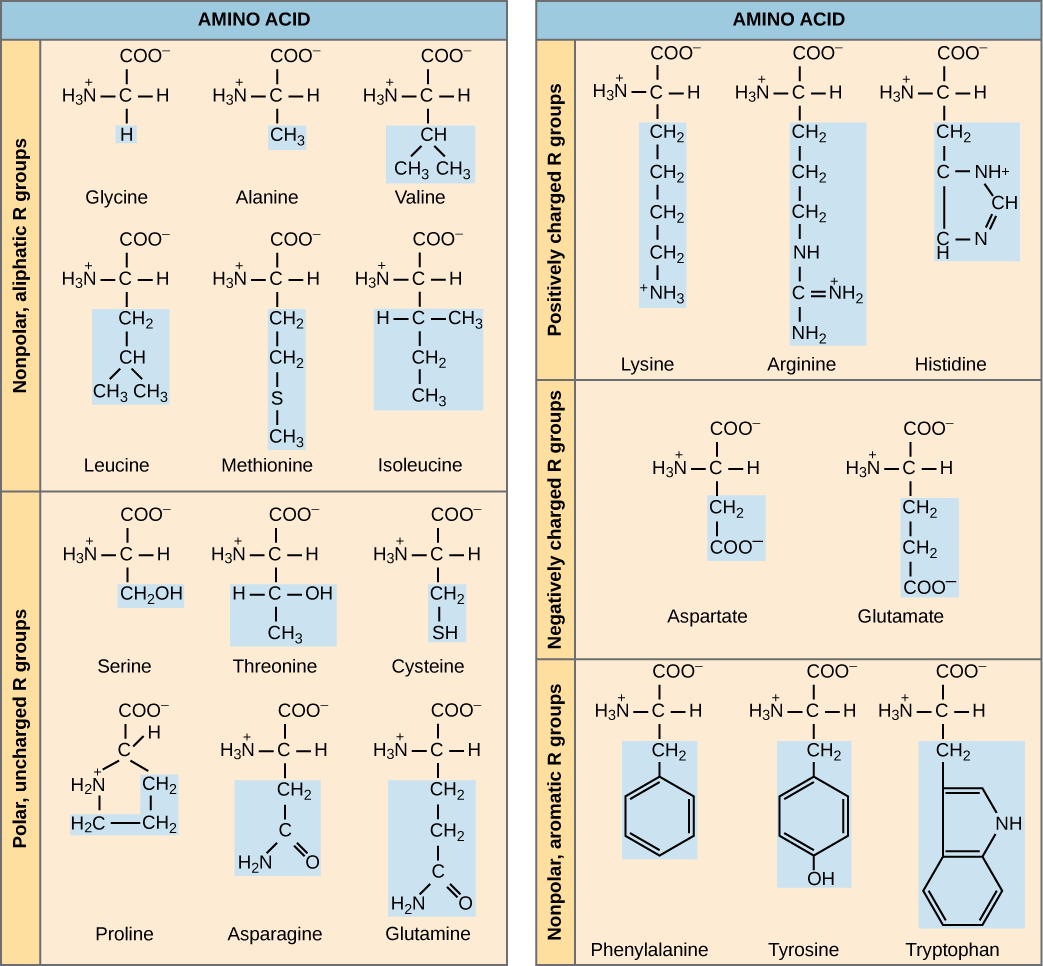
\includegraphics[width=0.8\textwidth]{aminoacids2.png}
  \caption{CAPTION AND REFERENCE}
  \label{fig:aminoacids}
\end{figure}

Two aminoacids are joined together through the formation of a peptidic (covalent) bond between them. Such a linkage is formed by removal of the elements of water (dehydration) from the $\alpha$-carboxyl group of one amino acid and the $\alpha$-amino group of another \cite{Nelson2008}. The remaining $\alpha$-amino and $\alpha$-carboxyl groups are available for linkage to other aminoacids, and in this way peptidic chains or peptides can be created.

While there are 20 basic units that constitute the majority of naturally observable proteins, their side chains can be modified both by physiological processes and by experimental procedures cite. One frequent instance of such modifications is the oxidation of methionine.


\section{The protein-focused biotechnology industry}


Proteins carry out most of the cell\textquotesingle s molecular functions, they work as molecular agents that can perform an extremely wide range of tasks. The advent of biotechnology has sought to take advantage of this power, either by using proteins as present in natural conditions (wild type) or engineered by humans. This potential economic activity is carried out by several biotech companies, including Novozymes A/S (NZ).

\ac{NZ} is a company whose line of business consists of the development of enzymatic products performing chemical transformations in different industrial processes. The application of these products, instead of conventional chemical-based solutions, has the advantage that they require less chemical substances, potentially simplifying industrial processes, reducing their costs and their environmental impact. Notorious examples of such applications include waste-water treatment, household care and the baking industry.


The advancement of the way \ac{NZ} does protein research is thus key to place the organization ahead of its competitors. The refinement of the currently used tools and the development of new ones could be of great significance for the company. 

Protein research can be approached from different angles. This thesis exploited the combination of mass spectrometry (\ac{MS}) and proteomics workflows (see chapter \ref{chap:mass_spec}) for the qualitative and quantitative characterization of protein samples.



\section{Objectives of the Thesis}
\label{sec:objectives}

In line with the goal of making \ac{NZ} more competitive, this project aimed at the following objectives:

\begin{enumerate}

\item Develop an open-source, Linux based and easily deployable pipeline for the analysis of \ac{MS} data, starting at the raw high-throughput data files and ending in the  biological interpretation of the results.

\item Evaluate this pipeline with a benchmark dataset to assess if the pipeline is able to reflect the biological phenomena captured in the data.

\item Establish a label-free quantification probabilistic model that provides relative abundance estimates and a measurement of their uncertainty based on the available data.

\end{enumerate}

\section{Structure of the Thesis}

An overview over the \ac{MS} and following computational data analysis steps is presented in \ref{chap:mass_spec}. The pipeline development and its benchmark are explained in chapters \ref{chap:pipeline} and \ref{chap:benchmark}, while the modelling problem is introduced in chapter \ref{chap:model}. Finally, a conclusion of the work is given in chapter \ref{chap:conclusion}.


\chapter{Mass spectrometry and shotgun proteomics overview}
\label{chap:mass_spec}

Life systems consist of complex systems, meaning their behaviour cannot be easily explained by analyzing the individual elements alone. Moreover, they present multiple layers of complexity, given by the nature of the elements that make it up. The layer provided by proteins is one of them, and its study is called proteomics. It is a complex layer because thousands of different proteins can be present in a single cell at any time, and their exact composition and quantities constantly change, responding to the stimuli of the surrounding environment. The study of the protein-specific complexity is called proteomics. With proteomics, one endeavors to infer the protein composition of a sample, and eventually quantify its protein amounts.

%CITE 1.6.1 COMPUTATIONAL METHODS.
The existing approaches are divided into two types of paradigms: top-down and bottom-up. In the top-down paradigm, intact proteins are directly used for the analysis. In the bottom-up paradigm (see figure \ref{figure:proteomics_overview}, the proteins are first cleaved into smaller parts, and these parts are then used for identification, characterization, and quantification. These smaller parts are called peptides. \cite{Barsnes2008}  Such peptides acquire physicochemical properties fitting the requirements of the downstream analytical methods, mainly the mass spectrometer (MS), which performs the data acquisition. The bottom-up paradigm is most often used because peptides are much more suitable to analysis by mass spectrometry, as explained in \ref{subsec:the_detector}. The top-down paradigm will be ignored in the rest of the manuscript.

\begin{figure}[!h]
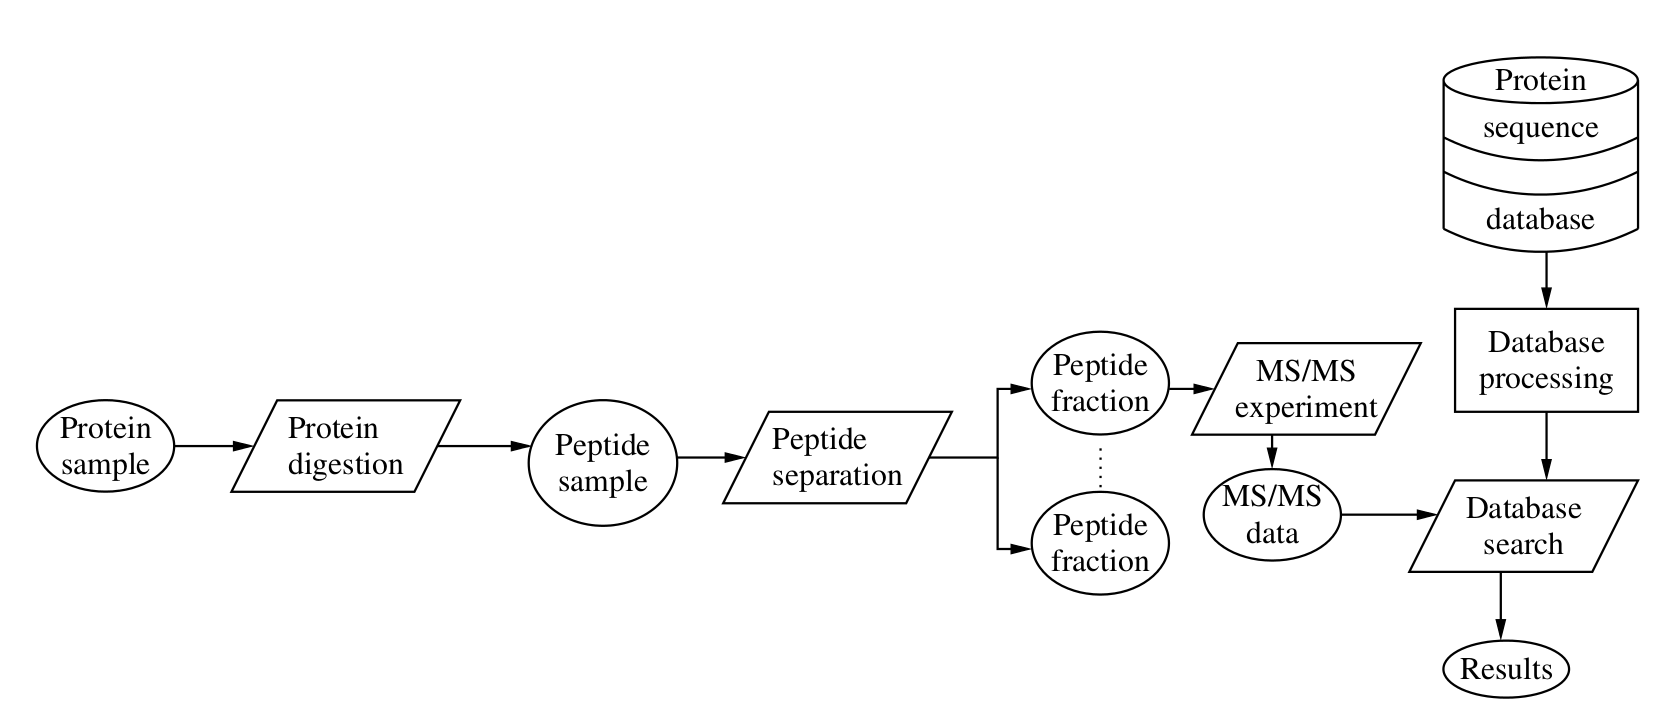
\includegraphics[width=\textwidth]{proteomics_skema_book}
\caption{Overview of a standard bottom-up proteomics analysis. Figure 1.3 from \cite{Barsnes2008}.}
\label{fig:proteomics_overview}
\end{figure}

MS is performed by means of a mass spectrometer, an ensemble of pieces of equipment that can acquire mass measurements for plenty of sample components. A detailed explanation of the sample processing required prior to MS is given in section \label{sec:sample processing}, while an overview on mass spectrometers is given in section \label{sec:the mass spectrometer}. The result of the MS analysis is a dataset that, with adequate computational analysis tools, is enough to perform the inference steps required to gather knowledge about the original protein sample. These inference steps can be condensed to the peptide and protein inference problems, explained in section \label{sec:peptide and protein inference}. A third computational problem needs to be solved if quantitative, and not just qualitative information, is to be gained from the experiment. This is the quantification problem, explained in section \ref{sec:quantification}.

A summary of the bottom-up approach MS analytical pipeline is provided in the rest of the chapter. It can be divided into two main steps:

\begin{enumerate}

\item \ac{MS} analysis and data generation. Sections \ref{sec:sample_processing} to \ref{sec:tandem_ms_workflow}.

\item Computational analysis of data. Sections \ref{sec:search_engines} to \ref{sec:quantification}.

\end{enumerate}

\LARGE
\textbf{MS analysis and data generation}
\normalsize

\section{Sample processing}
\label{sec:sample_processing}

\begin{figure}[!h]
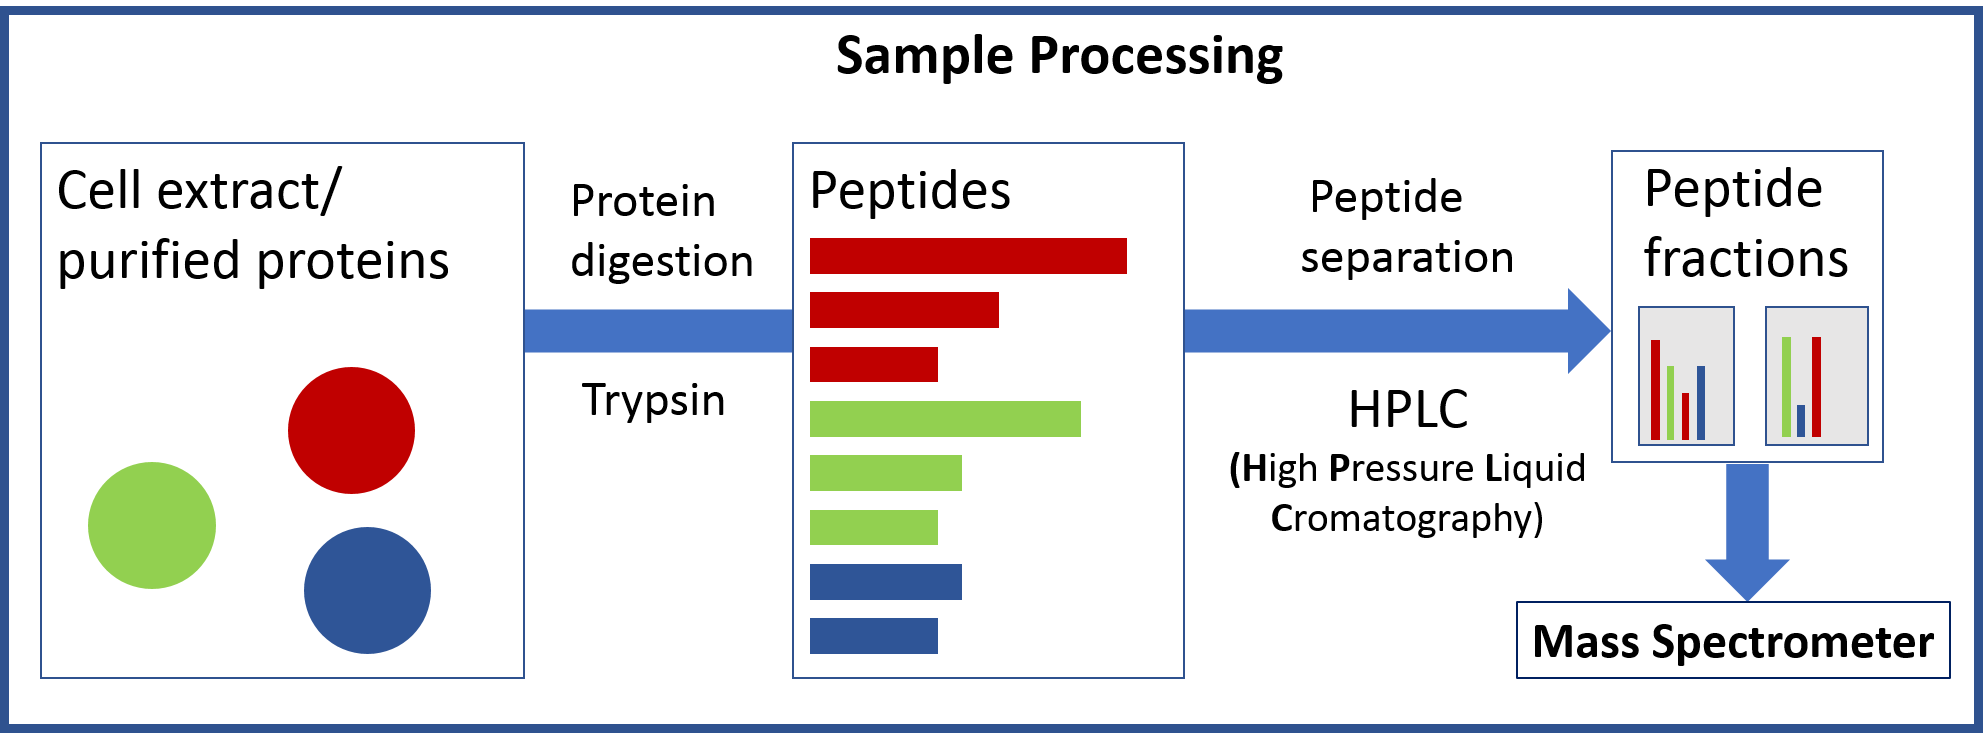
\includegraphics[width=\textwidth]{sample_processing}
\caption{Overview of the sample processing step prior to mass spectrometry analysis. First, proteins are denatured and digested with a specific protease like Trypsin. This yields a peptide mix that is separated into peptide fractions that can be introduced in the mass spectrometer.}
\label{fig:sample_processing}
\end{figure}

\subsection{Protein digestion}
\label{subsec:protein_digestion}

An \ac{MS} experiment starts with the generation of a protein sample from the biological system of interest. Proteins are then denaturalized  so as to remove bias due to the divergent properties acquired by folded proteins. Then, proteins are subjected to digestion with specific enzymes, which cut the aminoacidic chains following a predictable pattern. Trypsin is the most frequently used for this task. It cuts peptidic bonds whenever a positively charged residue, either Lysine (K) or Arginine (R), lies on the carboxyl side of the peptidic bond. Since roughly 1/10 residues are either R or K, the average peptide length is 10 residues. As explained in \ref{subsec:the_detector}, this length distribution is fitted to the resolution of the MS analyzer. Moreover, since R and K are positively charged aminoacids, the resulting peptide is guaranteed in most cases to be able to capture at least one charge, thus making it visible in the spectrometer. All of these properties combined, together with its low prize, makes Trypsin the enzyme of choice in this step for most cases.

Even though enzymes are very specific, the cleaving process is far from perfect, as there could be: \cite{Barsnes2008}
%COMPUTATIONAL METHODS 3.2

\begin{enumerate}

\item Missed cleavages.

\item Unsuspected cleavages during the maturation/life cycle of the protein.

\item Unexpected cleavages occurring either in the wet-lab procedure of the proteolytic treatment.

\item Naturally occurring, intentionally or unintentionally induced chemical modifications.

\end{enumerate}

%\Cref{item:missed_cleavages}

Missed cleavages can happen due to steric impediments or the presence of specific aminoacids that can weaken the enzyme\textquotesingle s function. This is the case of Trypsin whenever the residue on the other side of the peptidic bond is Proline. Altogether, a variability is created in the cleavage process that, though limited, needs to be taken care of in downstream analysis, as it could introduce biases in peptide observability. 

The result of this process is a complex mix of peptides, made up by hundreds or thousands of different molecules, following a length distribution given by the cleavage sites frequency and each protein\textquotesingle s aminoacidic composition. A peptide separation step is required before introducing the sample in the spectrometer.

\subsection{Peptide separation}
\label{subsec:peptide_separation}

If presented with the problem of analyzing a mixture of peptides, the capacities of mass spectrometers are easily overwhelmed by a too complex mixture, resulting in the analysis of only a minor part of the total protein of the sample. This can be surmounted by independently analyzing different fractions of the sample over time. The required sample separation is achieved by High-Performance Liquid Cromatography (\ac{HPLC}) methods, like reverse phase chromatography (separating on hydrophobicity) and strong cation exchange chromatography (separating on isoelectric point) \cite{Barsnes2008}.

%CITE 4.2 computational methods.
During \ac{HPLC}, the peptide mix loaded into a column containing a stationary and a solid phase. These phases create an environment where peptides interact differently based on their physico-chemical properties, set by the nature of the phases. The output of the column, called elute, will consist of subsets or fractions of peptides leaving the column at different retention times (\ac{RT}) i.e the amount of time passed before the peptide is observed in the mass spectrometer. Therefore, the input to the machine will consist of a simplified mix of peptides at a time.

\section{The mass spectrometer}
\label{sec:the_mass_spectrometer}

The mass spectrometer is the ensemble of pieces of equipment analyzing a peptide mix such as those generated following the workflow enunciated in sections \ref{sec:sample_processing} and \ref{subsec:peptide_separation}. It consists of three main parts: an ion source, a mass analyzer, and a detector (see figure \ref{fig:mass_spectrometer}).

\begin{figure}[!h]
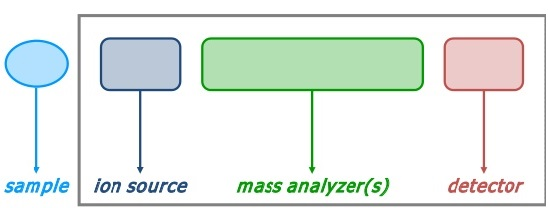
\includegraphics[width=\textwidth]{mass_spectrometer}
\caption[]{Schematic view of a mass spectrometer. Taken from \footnotemark{}}
\label{fig:mass_spectrometer}
\end{figure}

\footnotetext{\href{https://www.slideshare.net/joachimjacob/bits-introduction-to-mass-spec-data-generation}{https://www.slideshare.net/joachimjacob/bits-introduction-to-mass-spec-data-generation}}
\stepcounter{footnote}

\subsection{The ion source}
\label{subsec:the_ion_source}

All mass spectrometers exploit the physical properties of mass and electric charge exhibited by the analyzed components. Ionization of the analytes is absolutely essential prior to any measurement, as analytes left uncharged will be unobservable to the equipment.

%CITE 5.1 COMPUTATIONAL METHODS

This step is performed in the ion source \cite{Barsnes2008}. The most frequent ionization methods in proteomics are Matrix-Assisted Laser Desorption-Ionization (\ac{MALDI}) and Electro Spray Ionization (\ac{ESI}) \cite{Mirzaei2016}. Most peptides ionized by MALDI will acquire a single charge, whereas ESI can provide multiple charges (+2, +3, etc) too. Thus, the charge exhibited by an ion is not obvious when produced via ESI. Moreover, ESI can be run online with the right robotic equipment, while MALDI demands waiting time for vacuum generation. Finally, due to the chemical nature of the matrix components, MALDI ionizes more easily peptides containing aminoacids featuring aromatic rings (PYW), thus introducing a bias. Bias in ESI is less predictable. This is known as the competitive ionization problem \cite{Tang2004}.

The acquired charge yields a mass/charge (\ac{m/z}) ratio, a property that is applied in the downstream component separation and measurement steps.

\subsection{The mass analyzer}
\label{subsec:the_mass_analyzer}

The plethora of ion separation methods is reflected upon the range of different analyzers available, mainly time of flight (\ac{TOF}), Ion trap (\ac{IT}) and quadrupole (\ac{Q}). These apply different principles to perform the same task: separation (analysis) of the ion mix by the \ac{m/z} ratio.

Moreover, two other analyzers exist which combine mass analysis with intensity measurement. These are Fourier Transform Ion Cyclotron Resonance (\ac{FT-ICR}) and Orbitrap. They both register cylotron resonance frequencies that are Fourier transformed into the spectrum space. Remarkably, \ac{FT-ICR} exhibits great resolving power, at the cost of high maintenance costs and difficult operability \cite{Barsnes2008}. 

\subsection{The detector}
\label{subsec:the_detector}

Detectors measure the intensity of an incoming ion signal. The ion\textquotesingle s \ac{m/z} ratio is known thanks to the previous mass analysis step. Performed for enough \ac{m/z} ratios, the detector can produce a \ac{MS} spectrum, which shows the intensity of ion current over an \ac{m/z} range. Some topics in signal detection in \ac{MS} need to be discussed.

On the one hand, the precision of the signal measurement is given by its mass resolution It is conventionally defined as the closest distinguishable separation between two peaks of equal height and width \cite{Marshall2013}. The resolution decreases as the \ac{m/z} ratio increases because small increments in the \ac{m/z} ratio become negligible at high \ac{m/z} ratios. This is one of the reasons why proteins are better fit for analysis when digested into peptides, as \ac{m/z} are reduced, thus increasing the mass resolution.

On the other hand, due to the natural occurrence of isotopes, particularly \ce{^{13}_{}C}, the same peptide will induce the measurement of several signals with very close \ac{m/z} values. They constitute the isotopic envelope of the ion (see figure \ref{fig:envelope}), and represent the signal created by peptides containing an increasing number of \ce{^{13}_{}C} atoms. Every time a \ce{^{12}_{}C} is replaced by \ce{^{13}_{}C}, the mass increases by 1 Da. Even though the natural abundance of \ce{^{13}_{}C} is 1.1 \%, the sheer number of carbon atoms in a peptide makes it likely that at least one or even more carbon atoms will be \ce{^{13}_{}C}, eventually driving the pure \ce{^{12}_{}C} signal to comparatively small intensity values, and down to intensities below the background noise. Such event can be problematic if it entails that the \ce{^{13}_{}C} peak is confused for the \ce{^{12}_{}C} peak.

\begin{figure}[!h]
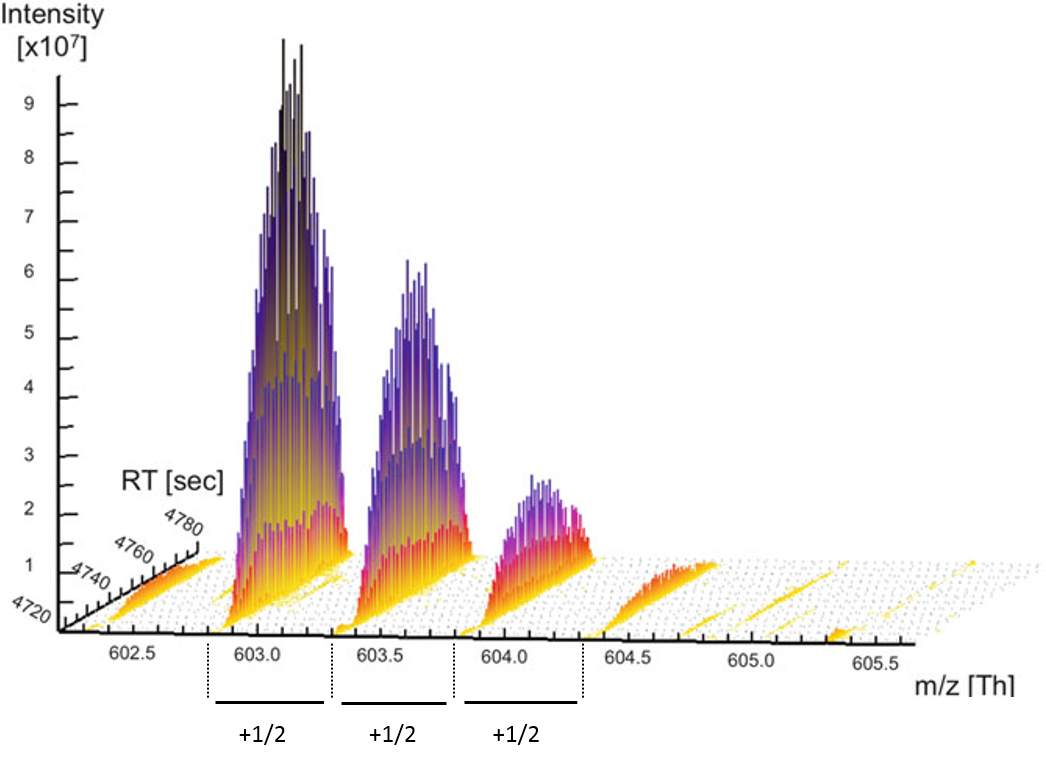
\includegraphics[width=\textwidth]{envelope}
\caption{A doubly charged isotopic envelope with its monoisotopic ion measured at 602.8 Th. Each peak in the envelope is separated by 0.5 Th. This is explained by the peptide having 2 positive charges that make every extra Da in the ion mass account for 1/2 extra Th. Adapted from \cite{Mirzaei2016}.}
\label{fig:envelope}
\end{figure}


The resolution achieved by modern equipment allows for the distinction of each individual signal in most isotopic envelopes. Remarkably, the separation across peaks in the envelope can be used to infer the charge of the peptide, as increases of 1 Da at charge 1 will induce a separation of 1 \ac{m/z}, while at charge 2 it will be $1/2 = 0.5$ \ac{m/z}, at 3 $1/3 = 0.33$ \ac{m/z}, and so on (see figure \ref{fig:envelope}).

It is up to the \ac{MS} technician to decide on the best pieces of equipment according to their availability and particularities of the dataset.

\section{Tandem MS workflow}
\label{sec:tandem_ms_workflow}

\begin{figure}[!h]
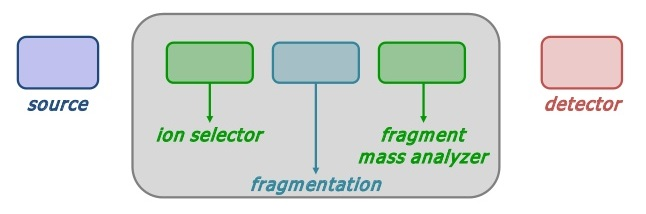
\includegraphics[width=\textwidth]{tandem_ms}
\caption[]{Illustration of the tandem MS workflow. The first spectrometer acts as an ion selector, that lets through ions with a given \ac{m/z} ratio. The second spectrometer does not perform mass analysis, but instead provides the medium where peptide fragmentation occurs. Finally the third spectrometer records fragment mass spectra. Taken from \footnotemark{}.}
\label{fig:tandem_ms}
\end{figure}

\footnotetext{\href{https://www.slideshare.net/joachimjacob/bits-introduction-to-mass-spec-data-generation}{https://www.slideshare.net/joachimjacob/bits-introduction-to-mass-spec-data-generation}}
\stepcounter{footnote}

Shotgun proteomics analyses make use of two or more mass spectrometers connected in series, giving rise to the so-called Tandem MS (\ac{MS/MS}) workflow. In this setting, each mass spectrometer collects a different type of spectra and thus different information (see figure \ref{fig:shotgun}. An extra spectrometer, usually a quadrupole, is introduced in between.

\begin{itemize}

\item The first spectrometer records the intensity versus \ac{m/z} ratio of the peptides eluting from the column at a given time and is used to filter ions exhibiting a selected \ac{m/z} ratio.

\item The ions filtered in the first spectrometer undergo fragmentation in the second spectrometer. %, as explained in \ref{subsec:fragmentation}.

\item The last spectrometer records the intensity versus \ac{m/z} ratio of the fragments produced in the previous step. The produced spectrum can be use to read out the peptide sequence.

\end{itemize}

\begin{figure}[!h]
\centering
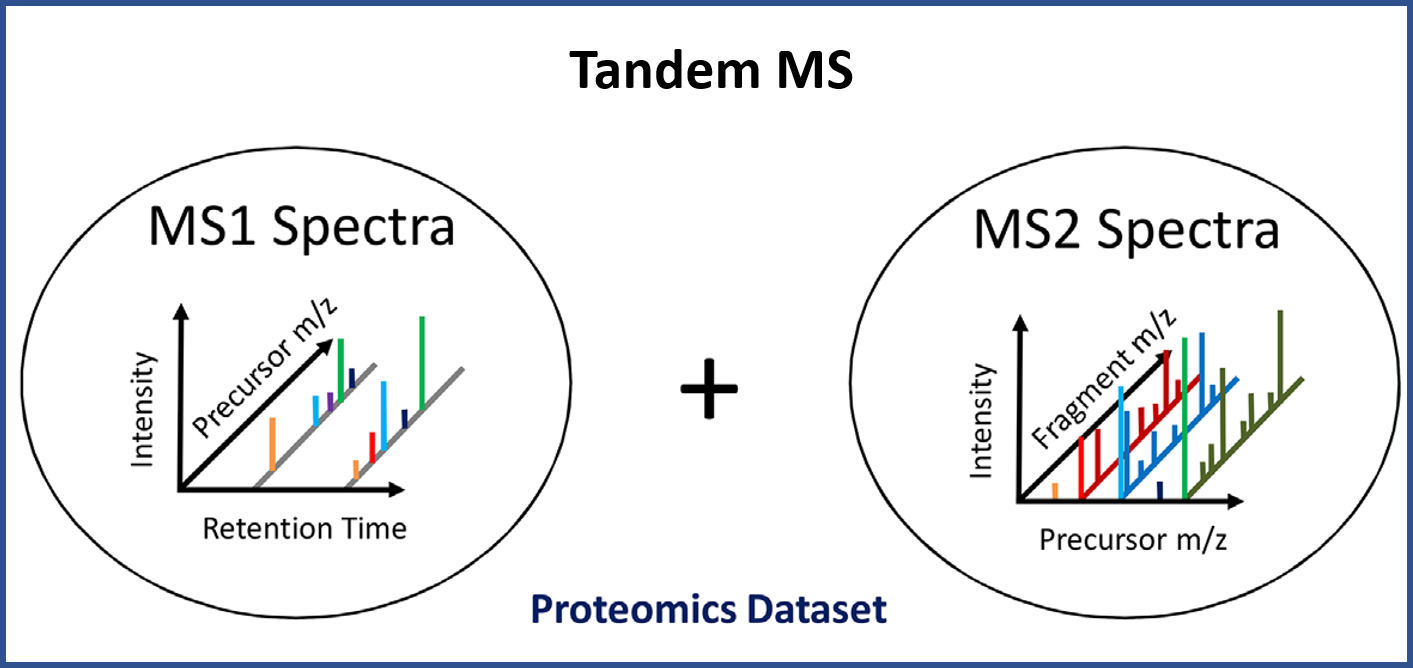
\includegraphics[width=\textwidth]{shotgun_adapted}
\caption{Illustration of the different spectra collected in tandem MS. MS1 spectra record precursor intensity vs \ac{m/z} ratio at different times. MS2 spectra record the same magnitudes but the signal is generated by the fragments produced during fragmentation by the ion filtered in the first spectrometer. Altogether, they enable peptide identifications. Figure adapted from \cite{Verheggen2017}.}
\label{fig:shotgun}
\end{figure}

\subsection{Fragmentation}
\label{subsec:fragmentation}

The information that can be extracted from \ac{MS1} scans consists of the \ac{m/z} ratio and retention time of the peptide ion, but not its sequence. Having the latter is paramount if the spectrum is to be matched to a theoretical peptide.

\begin{figure}[!h]
\centering
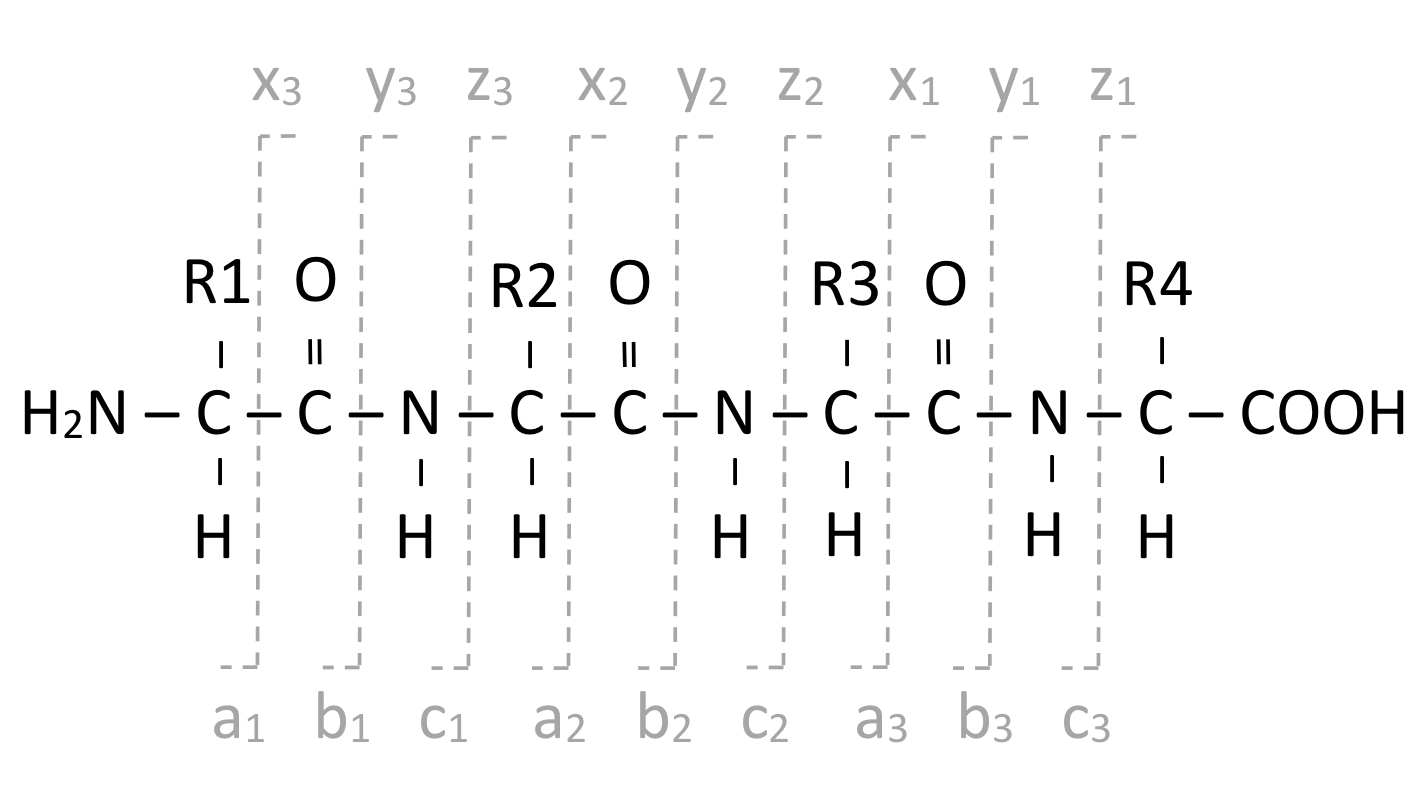
\includegraphics[width=0.8\textwidth]{abcxyz}
\caption{The common fragments and their relation to the peptide sequence can be organized into 2 groups of 3 series each. The abc fragments keep the N-terminal residue, while xyz keep the C-terminal one. Specific fragmentation techniques make fragments belonging to one series more likely than others. Other fragments are possible but much less likely. The fragment nomenclature was introduced in \cite{Roepstorff1984}.}
\label{fig:abcxyz}
\end{figure}


Fortunately, the peptide sequence of the ion can be inferred if fragmentation is performed. During peptide fragmentation, bonds along the peptidic chain are broken, turning the peptide into smaller fragments. These fragments will consist of truncated versions of the original peptide at different positions, thus making it possible to read an \ac{m/z} ratio difference between any pair of fragment ions. The difference can be exploited to infer which aminoacid is present in the longer fragment. If this process is repeated for enough pairs of contiguous fragments, with the right software, a sequence can be read from the \ac{MS2} spectrum.  explained in \ref{sec:search_engines}.

%A given bond will be more likely to break the less stable it is. This makes (I) the \ce{C_$\alpha$}-\ce{CO}, (II) the peptidic \ce{CO}-\ce{NH}, and (III) the \ce{C_$\alpha$}-\ce{NH} bonds the most likely to break (see figure \ref{fig:abcxyz}). A nomenclature REF was introduced to name these fragments:



%%PAG 123 COMPUTATIONAL METHODS
%Fragmentation in proteomics is performed via (I) collision-induced (CID) or (II) electron-induced (EID) dissociation. CID is an ergodic fragmentation technique where peptides enter a collision cell containing an inert gas. Given enough kinetic energy, hits between ionized peptides and the gas will trigger the fragmentation of the peptide into smaller units. \cite{Barsnes2008}. Since the kinetic energy is randomly distributed across the peptide, the weakest bonds will break first. This results in the production of mostly b and y fragments, as well as the loss of any chemical modifications \cite{Barsnes2008}.
%
%%CITE pag 134 computational methods
%
%EID is produced by the hits against the molecule, which tend to occur on the areas of the peptide more positively charged. Thus, the fragmentation process is not ergodic and returns TYPE ions. More importantly, chemical modifications are not lost in the process.
 
 
\LARGE
\textbf{Computational analysis}
\normalsize

\section{Spectra processing: search engines}
\label{sec:search_engines}

Computational analysis of MS data starts with the matching of the spectra to a referene proteome (see figure \ref{fig:computational_analysis}). \ac{MS} search engines are capable of performing the crucial step of peptide to spectrum matching (PSM). During this step, search engines perform \textit{in silico} prediction of the peptides produced in the protein digestion step and their expected spectrum.


\begin{figure}[!h]
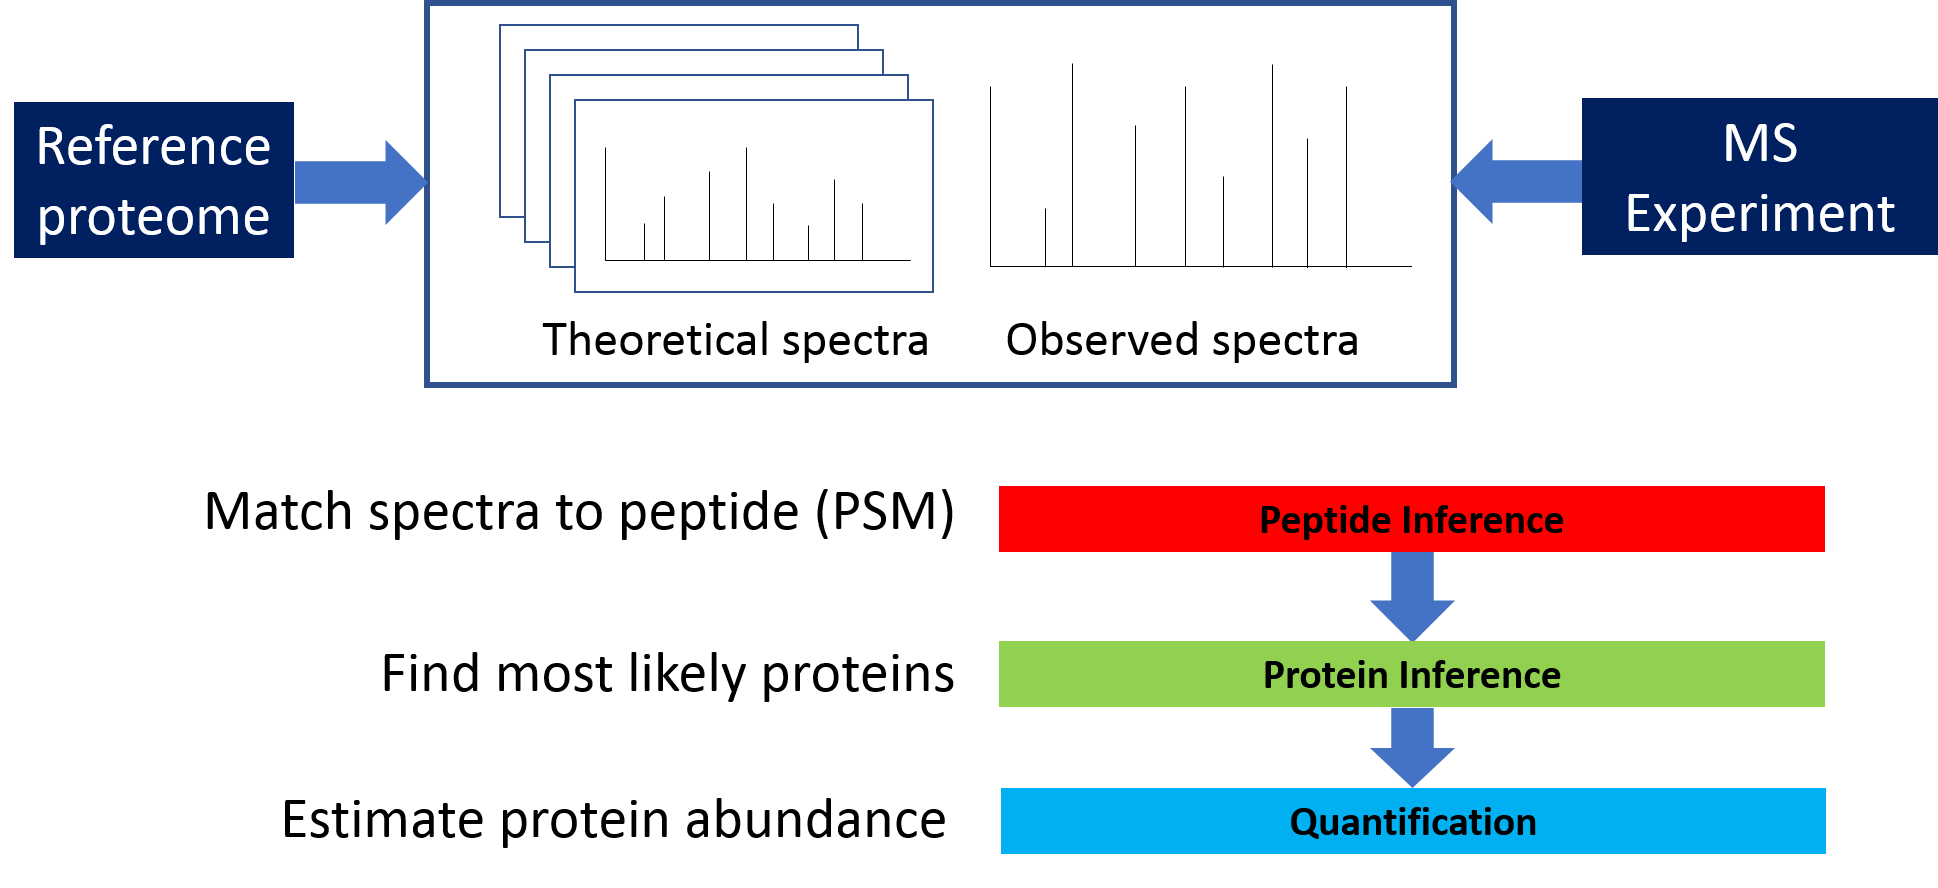
\includegraphics[width=\textwidth]{computational_analysis}
\caption{Diagram of the MS computational analysis. The PSM process maps the observed spectra to a list of peptides in the reference proteome that could have generated them. In other words, the software infers what peptides were introduced in the spectrometer. The analysis continues during protein inference and quantification.}
\label{fig:computational_analysis}
\end{figure}

%\begin{figure}[!h]
%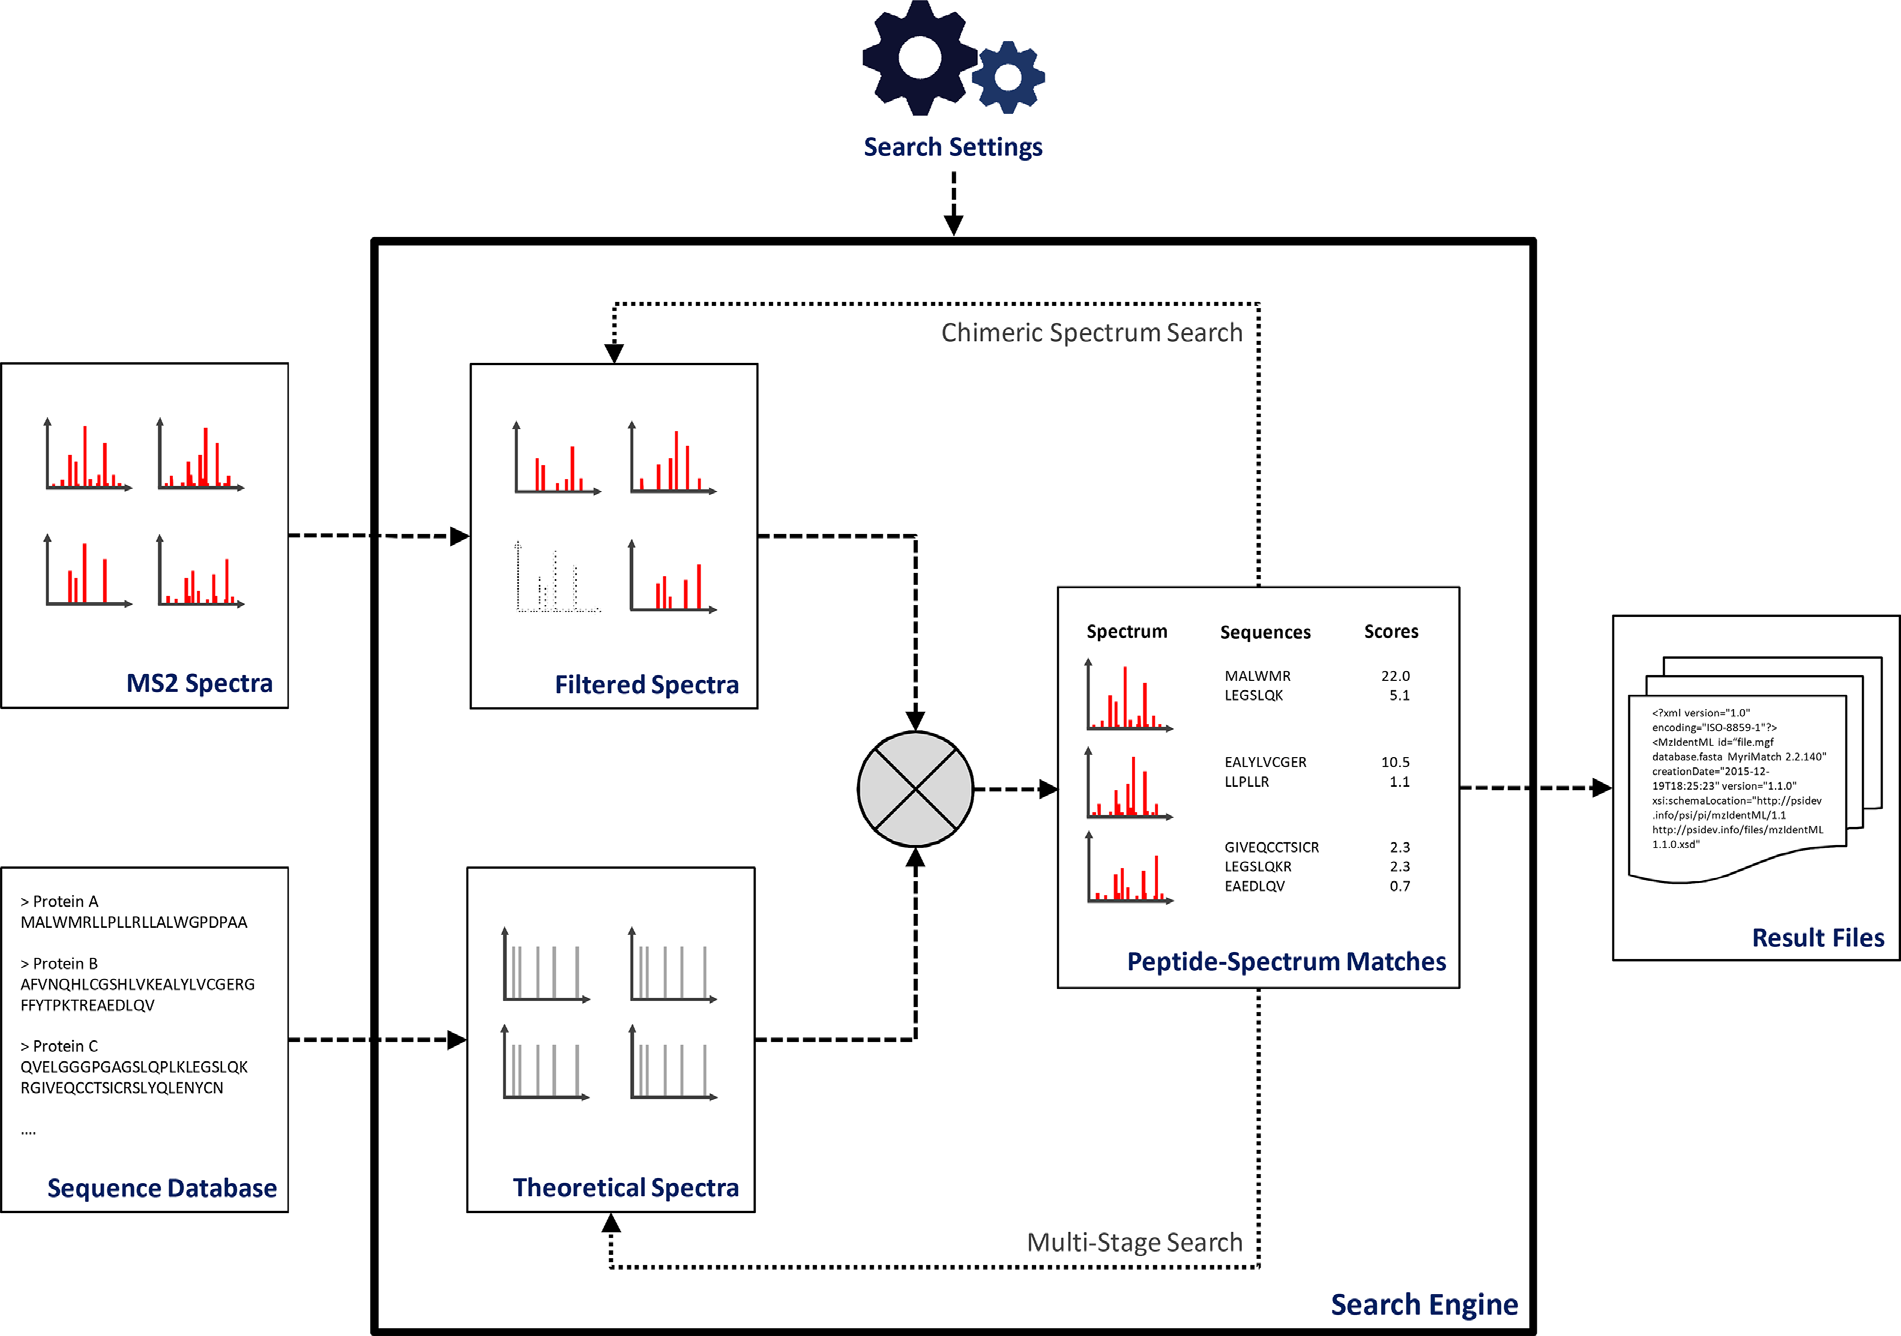
\includegraphics[width=\textwidth]{PSM}
%\caption{}
%\label{fig:PSM}
%\end{figure}

Given the stochastic nature of the protein cleavage and spectra recording processes, the resulting spectra exhibit variability manifested in missing peaks or spurious ones. Furthermore, random (wrong) matches can be returned by the PSM process when running against a sufficiently big database. This translates to the generation of multiple matches, of which one, if any, will be correct. Therefore, the lists of matches need to be somehow ranked by goodness-of-fit. The issue is addressed by search engines through the deployment of statistical models that provide scoring systems. Assuming the correct protein is present in the database, a good scoring system should give the best score to the right peptide. Under this circumstances, if repeated for several peptides, enough evidence for the presence of individual proteins can be collected.

Multiple search engines exist that implement different matching and scoring algorithms. The most modern ones include MS-GF+, MS-Amanda, Comet, X!Tandem or Andromeda. Notably, the results of each individual search engine can be combined to gather their strengths, at the expense of an increased computational cost and time \cite{Shteynberg2013}.



\section{Validation and quality control}
\label{sec:validation}

The scoring systems implemented in search engines provide the best matches, but they are bound to contain false identifications. Nevertheless, these scores can be used to apply a filter that aims at minimizing the amount of errors.

A common filter is the false discovery rate (FDR), usually set to 1\%, indicating that after the its application, only one out of a hundred filtered matches are expected to be false positives (wrong matches).

The most commonly used method to compute the \ac{FDR} of a list of matches is the target-decoy search. Using this method, the search engine replicates the matching process, using the same spectra, but instead against a decoy database. The decoy database is generated by reversing or more generally applying a randomization technique upon the sequences present in the original database (target). 

All matches to the decoy are by definition wrong. Since the basic properties of the decoy (size, composition, etc) remain identical to those of the target the amount of matches to the decoy exhibiting more than a given score $s$ can be regarded as an estimate of the number of false identifications ($\hat{n}_{fp}$) in the list of target results exhibiting at least the same score. This is because the existence of shared properties entails that random matches are equally likely to happen in both databases \cite{Elias2010}. Together with the number of PSMs passing a given score in the target ($n_{tp} + n_{tp}$), the FDR can be computed using equation \ref{eq:fdr}.

\begin{equation}\label{eq:fdr}
FDR = \frac{\hat{n}_{fp}}{n_{fp} + n_{tp}}
\end{equation}

The equation tells us that we can compute the FDR at any score by counting how many decoy hits have a greater score ($\hat{n}_{fp}$), and dividing by the length of our target hits list. Thus, the score that makes the FDR equal to a predefined value, frequently 0.01 or 1 \%, can be computed and used as threshold for the target hits.

\begin{figure}[!h]
\centering
%\begin{subfigure}{.45\textwidth}
%    \caption*{A}
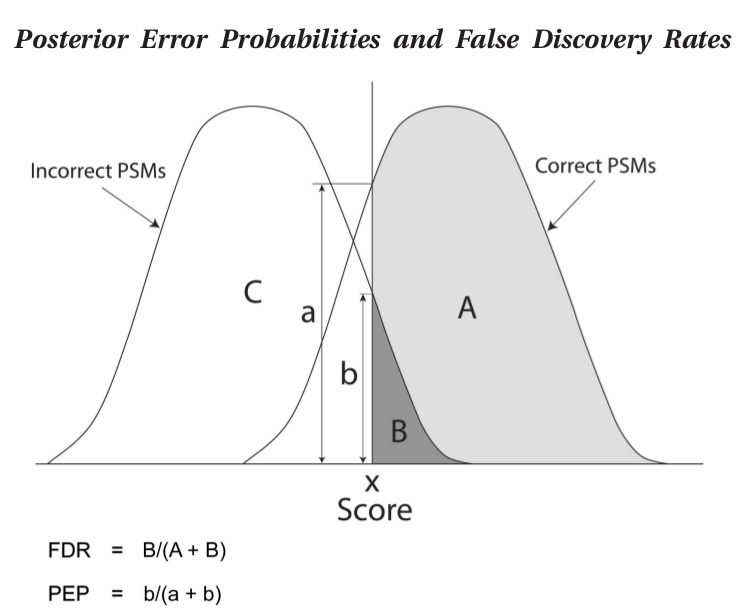
\includegraphics[width=0.9\linewidth]{pep}
\caption{Visualizing FDR and PEP. The FDR is defined as the ratio between False Positives and the sum of True and False Positives found in the list of PSMs of score greater than s. The PEP corresponds to the same ratio, but only a specific score, hence its alternative name of local-FDR. Figure from \cite{Kall2008}.}
\label{figure:pep}
\end{figure}


The minimal FDR at which a given PSM is considered a valid match constitutes the PSM\textquotesingle s q-value, i.e it is the smallest FDR we can allow while still keeping the PSM. Related to the q-value, the Posterior Error Probability (PEP) is an estimate of the probability of a given PSM of being an incorrect assignment (see figure \ref{fig:pep}). The PSM\textquotesingle s confidence is just defined as $1-PEP$ \cite{Nesvizhskii2010}. PEP can be computed from the decoy search results and provides another useful measurement of the uncertainty in the target results.




\section{Peptide and protein inference}
\label{sec:inference}

Two steps in protein identification can be distinguished:

\begin{enumerate}

\item \textbf{Peptide inference}: infer the peptides present in the sample.
\item \textbf{Protein inferece \textit{proper}}: based on the inferred peptides, infer what proteins generated them. This is not trivial as peptides are degenerate and frequently map to more than one protein.
\end{enumerate}

The result of the PSM step returns the inferred list of peptides. The ensemble of proteins most likely to have generated the list of peptides stemming from the filtered PSMs can be inferred using different algorithms. The degenerate nature of peptides is dealt with the Occam\textquotesingle s razor principle, which states that the most likely solution is the simplest one. Thus, protein inference algorithms aim at explaining the maximum amount of peptides using the least amount of proteins.

\section{Protein quantification}
\label{sec:quantification}

The combination of all the aforementioned computational analyses yields a list of protein identities that reports the protein composition i.e qualitative information of the original sample. However, in most proteomics applications, quantitative data can be of great interest, as many biological phenomena are manifested mainly through changes in the protein abundances, rather than protein presence alone. For instance, cancer cells in response to a drug could modulate the abundance of several proteins without removing them from the cytosol or introducing new ones.

Protein quantification pipelines can be classified based on whether isobaric labelling was used (label-based) or not (label-free). These are explained in subsection \ref{subsec:labelling}. If the label-free approach is employed, more distinctions can be made based on:

\begin{itemize}
\item The proxy used for quantification: spectral counting (\ac{SC}) or extracted ion currents (\ac{XIC}). These are explained in \ref{subsec:scvsxic}


\item The way the data are brought to the protein level from the peptide level: summarization-based vs. peptide-based, explained in \ref{subsec:peptide_model}.
\end{itemize}

\subsection{Label-based and label-free approaches}
\label{subsec:labelling}

%CITE PAGE 237 COMPUTATIONAL METHODS 

Two paradigms exist in protein quantification: label-based and label-free. In label-based quantification, originally identical peptides from a number of different samples are made distinguishable by their masses via the incorporation of a label. All label-based methods simultaneously analyze several samples in each experiment, removing the difficulties associated with between-run variability \cite{Barsnes2008}. The finite number of "plexes" available for a given label sets the limit to how many samples can be differentially quantified \cite{Cox2014}. Different techniques, like Stable Isotope Labeling by Amino acids in Cell culture (SILAC) or Isotope-Coded Affinity Tags (ICAT), differ in the nature of the label and the way it is introduced. Remarkably, peptide labeling costs can be quite high. This, together with the limited amount of samples that can be compared makes a case for label-free quantification.

In the label-free quantification approach, peptides from different samples are not labelled differently and are thus distinguished by their presence in different, independent \ac{MS} runs. In order to account for the introduced inter-run variability in peptide identifications and \ac{RT}, a match-between-runs (MBR) processing step can be carried out (see figure \ref{figure:moff_mbr}). 


\begin{figure}[!h]
\centering
%\begin{subfigure}{.45\textwidth}
%    \caption*{A}
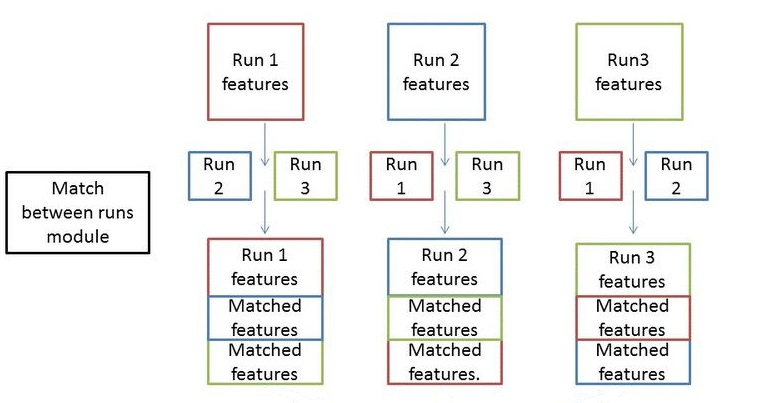
\includegraphics[width=0.9\linewidth]{mbr_workflow}
\caption{Illustration of the \ac{MBR} step. \textbf{A} the information gathered from matches in replicate runs is put to use during a reanalysis of the spectra. Modified from supplementary information in \cite{Argentini2016}.}
\label{figure:moff_mbr}
\end{figure}

This way, extra identifications are attained through a reanalysis of the spectra, factoring in the information collected in replicate runs. The RT and precursor mass of unidentified spectra in one replicate is matched to that of identified spectra in the remaining replicates. As a consequence, more identifications with a lesser fraction of missing datapoints are achieved.


\subsection{SC and XIC based quantification}
\label{subsec:scvsxic}


Quantification can be spectral counting or \ac{XIC} based.

On the one hand, spectrum counting based quantification is the simplest method in proteomics. It relies on the rationale that highly abundant peptides will have a higher intensity and are thus more likely to trigger the acquisition of MS/MS spectra. These methods have the advantage that they are very simple to implement and don't require any further data processing

On the other hand, \ac{XIC} based methods rely on intensity measurements at any level of the \ac{MS} workflow as proxies for protein abundance. A wide range of algorithms are available to process these data and output estimates of protein abundance. All of them require an intensive preprocessing step, usually including (I) taking the $log_2$ intensity to make the data distributions symmetrical and thus make it fit for diverse parametric tests, and (II) quantile normalization to address between-runs variability in the intensity measurements. They can be classified in the bases of which MS level is used as proxy for the protein abundances and on whether or not a summarization step is performed to aggregate peptide-level data into protein-level data, or not. 


As stated in \cite{Cox2014}, \textit{although the abundance of proteins and the probability of their peptides being selected for \ac{MS/MS} sequencing are correlated to some extent, \ac{XIC}-based methods should clearly be superior to spectral counting given sufficient resolution and optimal algorithms. These advantages are most prominent for low-intensity protein/peptide species, for which a continuous intensity readout is more information-rich than discrete counts of spectra}. For this reason, only the \ac{XIC} approach will be regarded in the rest of the manuscript.  

For a more robust XIC based quantification, a feature extraction step is usually executed to extract the apex intensity of the identified peak clusters, as shown in figure \ref{figure:moff_apex}.

\begin{figure}[H]
\centering
\begin{subfigure}{1\textwidth}
\centering
\caption*{A}
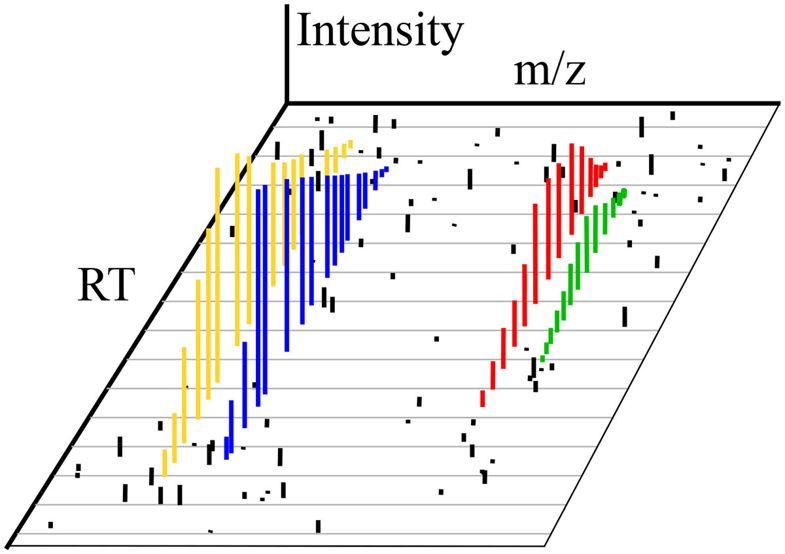
\includegraphics[width=0.7\linewidth]{apex_3d}
\end{subfigure}
\bigskip
\begin{subfigure}{1\textwidth}
\centering
\caption*{B}
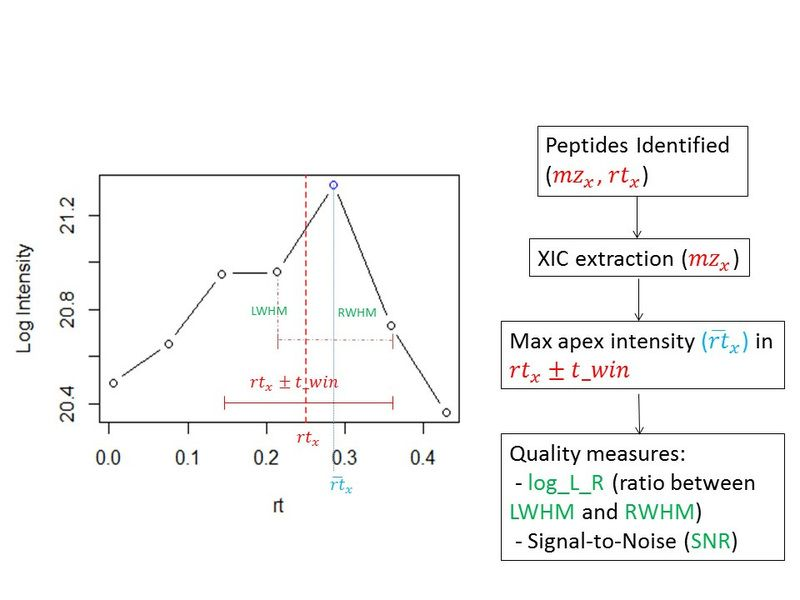
\includegraphics[width=0.7\linewidth]{apex_intensity}
\end{subfigure}
\caption{Illustration of the apex intensity extraction step.\textbf{A} Visualization of a 3D peak cluster on the RT / m/z plane. An ion current at the same m/z ratio, thus corresponding to the same precursor ion, is detected with varying degrees of intensity over a more or less narrow time window, spreading the signal over time. Taken from \cite{Smith2014}. \textbf{B} A refinement analysis of these data attempts to fit a mathematical model of the signal over time and extract a representative measurement, such as the highest (apex) \ac{MS1} intensity. Modified from supplementary information in \cite{Argentini2016}.}
\label{figure:moff_apex}
\end{figure}


\subsection{\ac{XIC}-peptide-based models for label-free quantification}
\label{subsec:peptide_model}

The data collected in the mass spectrometer refers to peptides originating from a latent protein composition, given by the original sample. However, the data interpretation requires the transfer of these peptide-level data into the protein level. This can be done by either (I) performing an aggregation of the peptide-level data, where a summary value of the peptide-level data is taken as representative for the protein-level data, or (II) performing the protein quantification directly at the peptide-level by means of linear regression models.

As stated in \cite{Goeminne2015} \textit{peptides originating from the same protein can indeed be considered technical replicates and theoretically should lead to similar abundance estimates. However, the summarization of the peptide intensities into protein expression values is cumbersome, and most summarization-based methods do not correct for differences in peptide characteristics or for the between-sample differences in the number of peptides that are identified per protein. This might introduce bias and differences in uncertainty between the aggregated protein expression values, which are typically ignored in downstream data analysis steps}.

It is for this reason that peptide-based models offer the statistical framework required to learn as much from the data as possible. This translates into improved results when compared to the other aforementioned methods \cite{Goeminne2015}. This hypothesis is the motivation for the method explained in chapter \ref{chap:model}.




\chapter{A label-free quantification proteomics pipeline}
\label{chap:pipeline}


\section*{Summary}

A pipeline making use of the set of tools published by the Compomics  and StatOmics groups SearchGUI, PeptideShaker, moFF and MSqRob, was developed to support complete label-free protein quantification analyses using the most recent advances in the field with open-source software. The pipeline can be run on Linux computer clusters to perform (I) peptide to spectrum matching against a reference database, (II) quality control and filtering, (III) MBR and feature extraction, (IV) protein inference and (V) relative quantification. Its output can be passed to follow-up analyses in R or Python to get a biological interpretation of the results.  A benchmark of its performance was accomplished using the proteome benchmark dataset published in \cite{Cox2014}. The results exhibited an accuracy similar to those achieved by the MaxQuant \cite{Cox2014} software, excepting a bias produced by the sample fractionation of this dataset.


\section{Introduction}

\begin{figure}[!h]
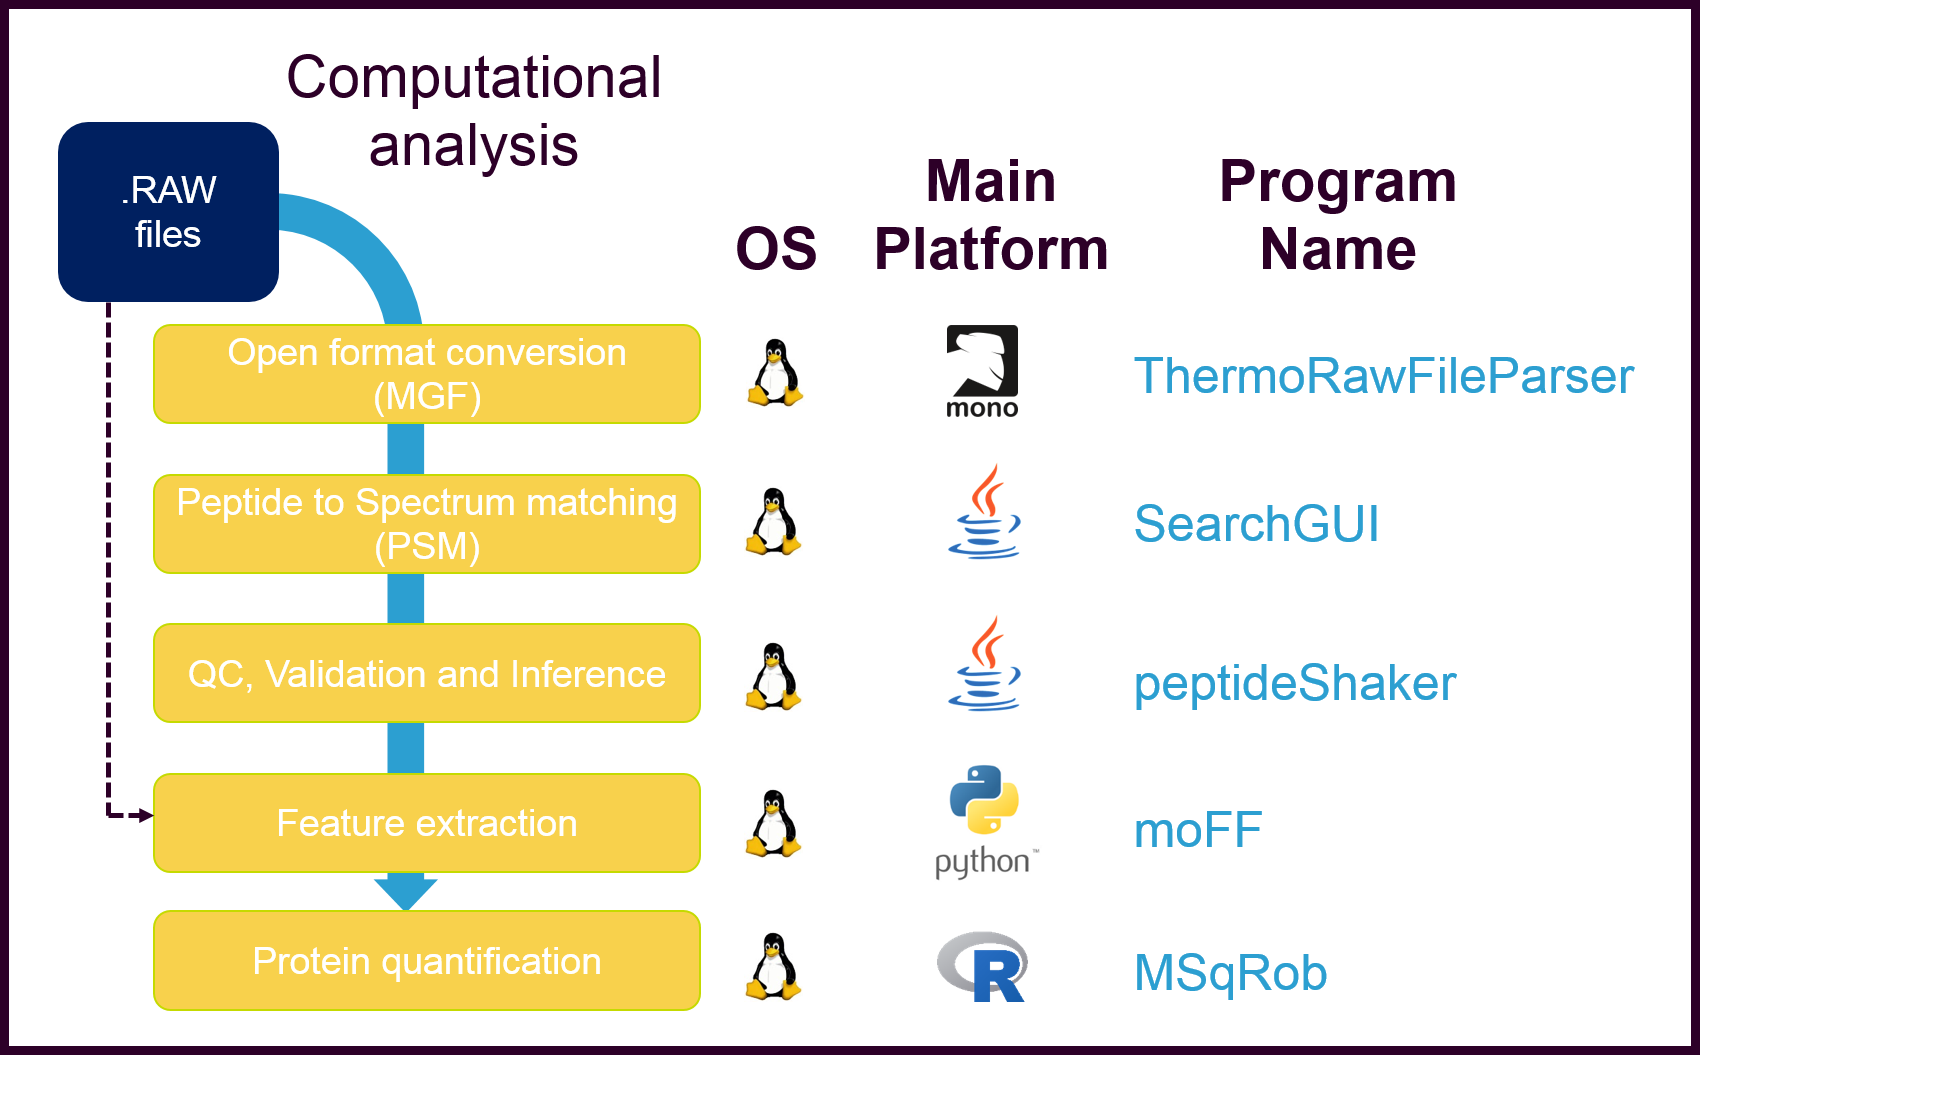
\includegraphics[width=\textwidth]{pipeline}
\caption{Schema of the presented pipeline. First, .RAW files produced by the spectrometer are converted to an open format like MGF. After that, spectra are searched by means of a search engine to perform the PSM step. Thereafter, PSMs are validated and the most likely set proteins is inferred. If quantative information is to be extracted, a quantification step attempting to estimate protein quantities is executed. The biological interpretation of the pipeline results can be achieved by interacting with public databases using R/Bioconductor or Python thanks to their open format.}
\label{fig:pipeline}
\end{figure}


Several proteomics pipelines are available on the internet under different licensing conditions. Many are released as closed-source software, where information on how the program works is kept from the user. This is a serious drawback as it hinders the study of the implemented models and its customisation. Open-source, free alternatives, like the Trans Proteomic Pipeline (\ac{TPP}) \cite{Deutsch2011} or openMS \cite{Sturm2008} are nevertheless available for the community. MaxQuant, a freeware but closed-source and monolithic proteomics analysis suite \cite{Cox2008}, has been extremely successfully adopted by the scientific community due to its ease of use and comprehensive pipeline.

However, still only few of these tools have a fully Linux-supported, well-documented, command-line version available, which would make customised, automatic streamline analyses much easier to perform. As a GUI would not be required to run the pipeline, it would also be scalable to big datasets. Finally, having free licenses would imply that anyone, provided the technical knowledge, can perform the computational analysis independently, thus speeding the data to knowledge turnover in \ac{NZ} or any organization making use of it.

The development of a pipeline attempting to achieve these goals will be described in this chapter.

\section{Materials and Methods}

\subsection{Data generation and loading}

The proteome benchmark dataset from \cite{Cox2014} was reanalysed starting at the output RAW files available at the PRIDE repository \footnote{\href{https://www.ebi.ac.uk/pride/archive/projects/PXD000279}{https://www.ebi.ac.uk/pride/archive/projects/PXD000279}}. Briefly, the \textit{Homo sapiens} and \textit{E. coli (strain K12)} proteomes were mixed in 1:1 (condition L) and 1:3 (condition H) proportions, with 3 replicates for each combination. Moreover, each of the 3 replicates of the 2 conditions was analysed over 24 fractions. This experimental setting thus generated a total of $2 \times 3 \times 24=144$ RAW files. One file was missing in the repository. The ThermoRawFileParser \footnote{\href{https://github.com/compomics/ThermoRawFileParser}{https://github.com/compomics/ThermoRawFileParser}} program was used to convert RAW files to the open format MGF (Mascot Generic Format).

The MQ+MaxLFQ pipeline results were obtained starting at the Supplemental table 1 from the MaxLFQ paper supplemental data \footnote{\href{http://www.mcponline.org/content/13/9/2513/suppl/DC1}{http://www.mcponline.org/content/13/9/2513/suppl/DC1}} \cite{Cox2014}, which is available as an excel file. The results of the MQ+MSqRob pipeline employed the Levenberg-Marquandt minimised peptide intensities stored in the peptides.txt file contained in the spectraHeLaEColi.zip in the supplemental data.

%\href{http://www.mcponline.org/content/suppl/2014/06/17/M113.031591.DC1/mcp.M113.031591-1.xlsx}{http://www.mcponline.org/content/suppl/2014/06/17/M113.031591.DC1/mcp.M113.031591-1.xlsx}.

\subsection{Decoy database preparation and search}

The spectra saved in the MGF files obtained in the previous step were passed to the MS-GF+ search engine CITE by means of the SearchGUI \texttt{SearchCLI} tool CITE utility. The search parameters were set using the \texttt{IdentificationParametersCLI}. In order to account for potential post-translational modifications, the search was conducted allowing for the following variable modifications: oxidation of M and deamidation of N and Q. Moreover, C carbamidomethylation was set as fixed modification. The enzyme was set to semispecific Trypsin, allowing for a non-tryptic cleavage on any side of the peptide. Up to two missed cleavages were allowed. The precursor tolerance was 10 ppm and the fragment tolerance 0.5 Da. 


The target database was created by combining the Uniprot proteomes for \textit{E. coli (strain K12)} (UP000000625) and \textit{Homo sapiens} (UP000005640), downloaded in June 2018. The decoy database was created using the \texttt{FastaCLI} utility in SearchGUI by reversing all sequences in the target.

\subsection{Quality control and validation}

The SearchGUI results were filtered using the default built-in checks available in the PeptideShaker utility \texttt{PeptideShakerCLI} \footnote{\href{https://github.com/compomics/peptide-shaker/issues/300}{https://github.com/compomics/peptide-shaker/issues/300}}. By default, the FDR was set to 1\%. PEP and confidence statistics were computed using the PeptideShaker built-in algorithms. Output was extracted via the Default PSM report txt file, available in the \texttt{ReportCLI} utility.


\subsection{Data refinement}

The moFF command line utility CITE was applied to perform (I) match-between-runs and (II) extract MS1 apex intensity of each peak cluster. This required passing the original RAW files, together with the Default PSM report from PeptideShaker. Output was exported to a peptide summary file, containing  one row per peptide and for every peptide, the detected apex intensity in each sample.

\subsection{Quantification}

Relative quantification was performed using the MSqRob utility by passing the peptide summary file from moFF. Prior to quantification, the data was preprocessed using the \texttt{preprocess\_MSnSet()} function. In a nutshell, (I) MS1 apex intensities were $log_2$ transformed, (II) quantile normalized, (III) peptides belonging to protein groups that contained one or more proteins that were also present in a smaller protein group were discarded \cite{Goeminne2016}, and (IV) protein groups with only 1 peptide were dropped.

Once preprocessing is done, a ridge regression model with Huber weights and empirical Bayes estimation of protein variance, implemented in the MSqRob package \cite{Goeminne2016}, was fit to every protein individually. The peptide and fraction effects were considered random, while the condition was treated as a fixed effect. The significance of the treatment effect differences was assessed through a Student\textquotesingle s T test, implemented in the \texttt{test.contrast()} function. Only protein groups that could be unambiguously mapped to one of the organisms were considered for the analysis.

Quantification in the MQ+MaxLFQ pipeline was executed using the LFQ intensity columns stored in the supplemental data file. Intensities were log2 transformed and averaged. The difference between conditions H and L was taken as estimate of the log2FC. Significance was evaluated by means of the two-tailed Welch Two Sample t-test implemented in the \texttt{t.test()} function in R. P-values were corrected using the FDR method implemented in the \texttt{p.adjust()} function in R.


\subsection{Code implementation}

\section{Results}

\subsection{Thousands of spectra were identified and validated}

The preprocessing of the RAW files produced by the mass spectrometer into the MGF open format enabled searchGUI to dispose of the registered spectra. PeptideShaker quality control and filtering capabilities (see figure \ref{figure:qc_validation}) carried out the required search results validation. As expected, matches to the target and decoy exhibited similar score distributions at low score values, while a divergence is observed at higher score values. Likewise, the m/z error was found to be closer to 0 on validated PSMs than on those which did not pass the 1 \% FDR filter. The application of this filter implied that the FNR (false negative rate) was set to 5 \%, i.e 5 out of every 100 discarded matches were estimated to be true positives.



\begin{figure}[!h]
\centering
\begin{subfigure}{.45\textwidth}
  \centering
  \caption*{A}
  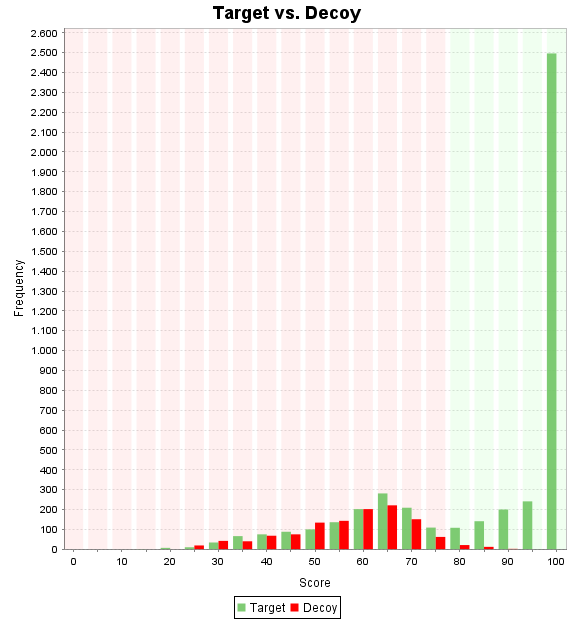
\includegraphics[width=.9\linewidth]{target_vs_decoy}
\end{subfigure}
\begin{subfigure}{.45\textwidth}
  \centering
    \caption*{B}
  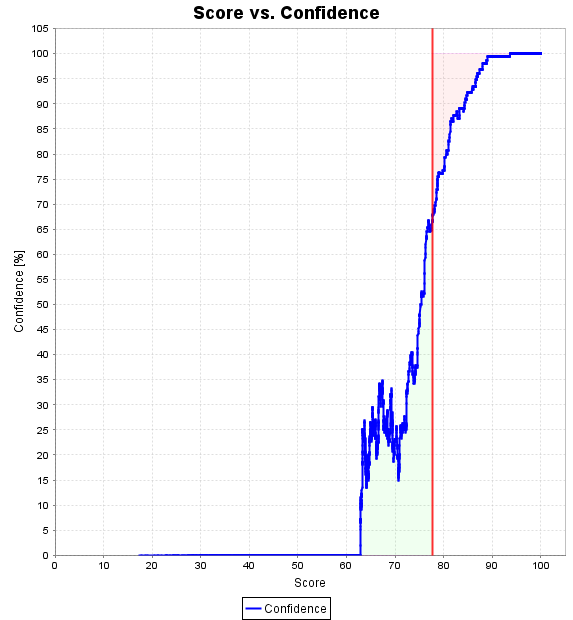
\includegraphics[width=.9\linewidth]{score_vs_confidence}
\end{subfigure}
\bigskip

\begin{subfigure}{.45\textwidth}
  \centering
    \caption*{C}
  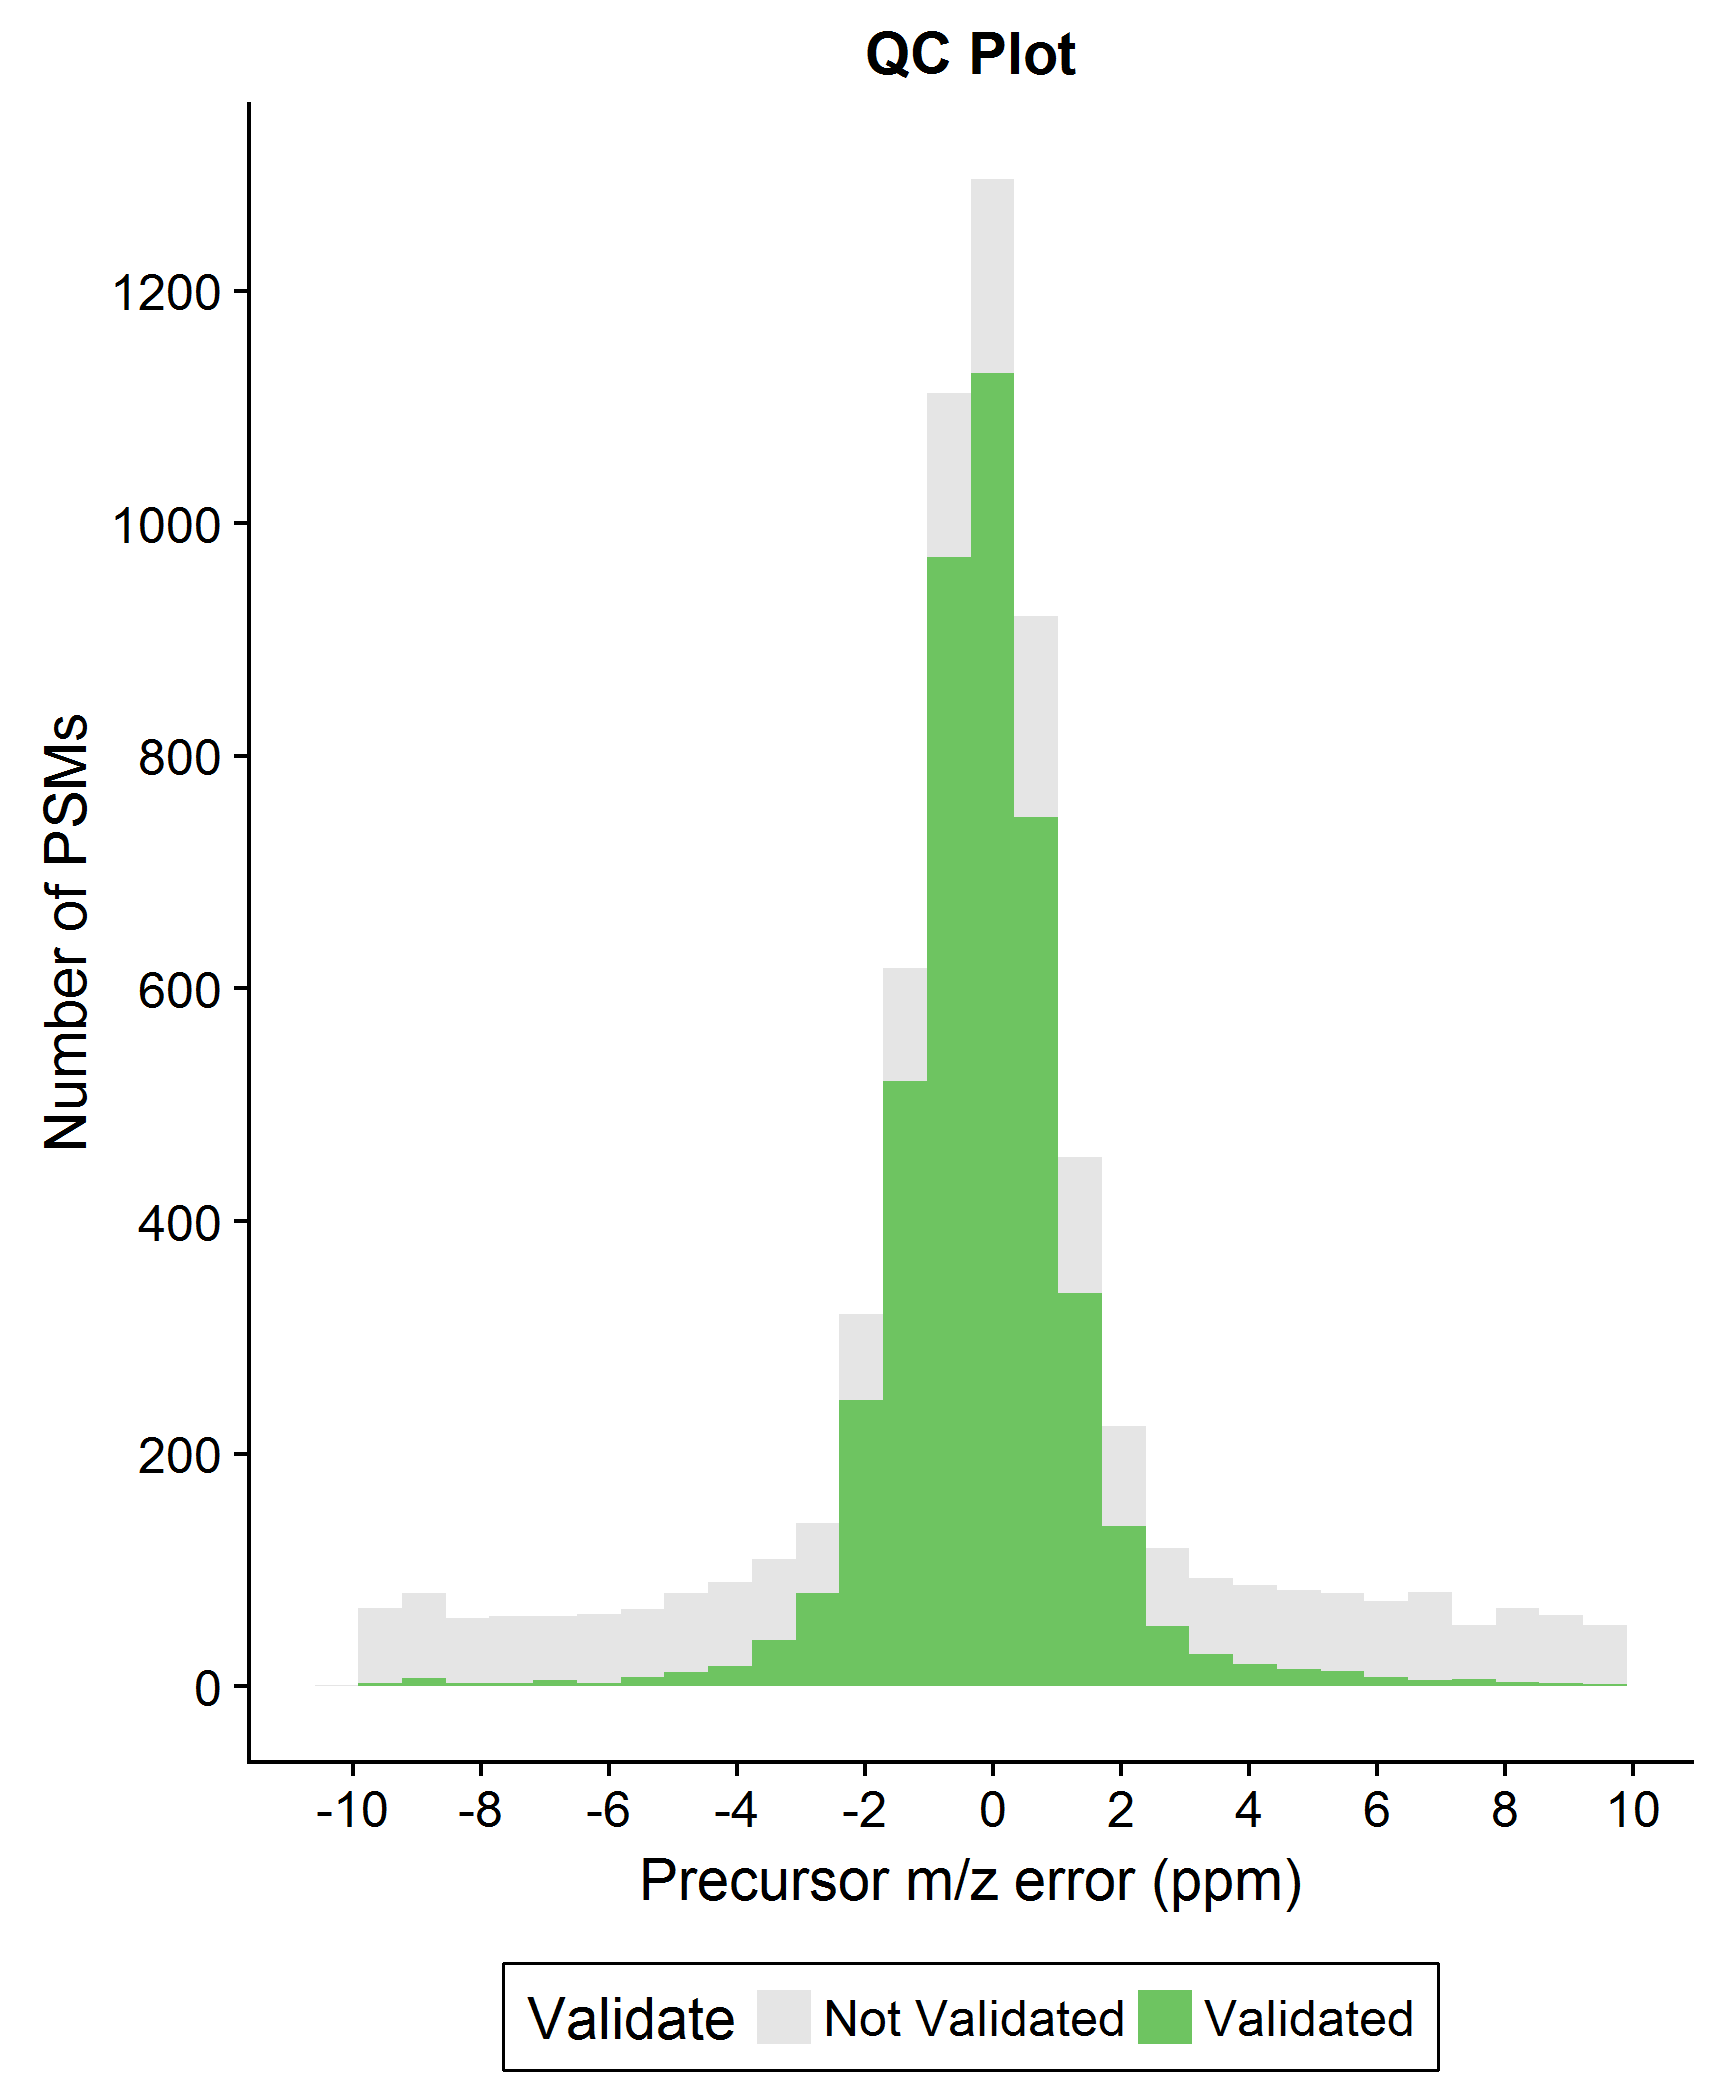
\includegraphics[width=.95\linewidth]{qc}
\end{subfigure}
\begin{subfigure}{.45\textwidth}
  \centering
    \caption*{D}
  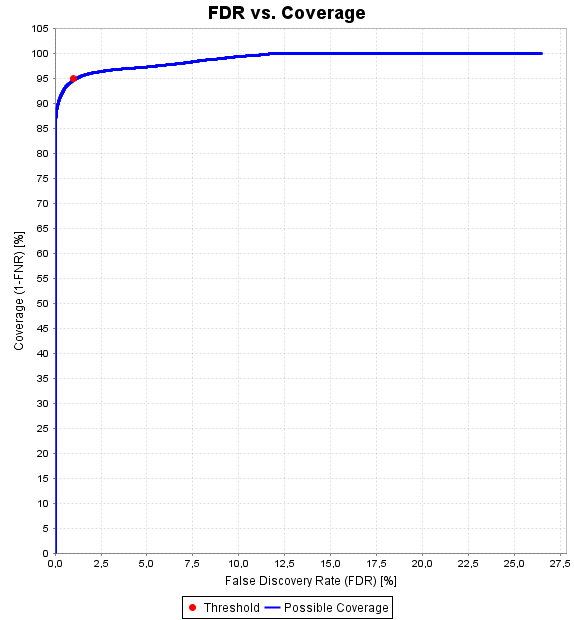
\includegraphics[width=.95\linewidth]{roc}
\end{subfigure}
\caption{Quality control and validation of the 13th fraction of the third replicate in condition L. \textbf{A} Score distribution for matches to the decoy and the target databases. \textbf{B} Evolution of the PSM score with confidence. The implemented cutoff at FDR of 1 \% is displayed with a red vertical line. \textbf{C} Distribution of the difference between the predicted and measured \ac{m/z} values, segregated by validation status. \textbf{D} ROC curve built upon the number of false positives and negatives estimated from the decoy search. The cutoff is displayed as a red dot.}
\label{figure:qc_validation}
\end{figure}

 The 1\% FDR cutoff selected PSMs with a score higher than 78, which translated to a confidence of at least 65\%.


The combination of both programs enabled the identification and validation (matching) of thousands of spectra with high confidence in all samples. However, when compared to the total amount of spectra available, the percentage of matched spectra was on average 37.4\%, with a marked decrease starting at fraction 14 (see figure \ref{fig:match_percent}).

\begin{figure}[!h]
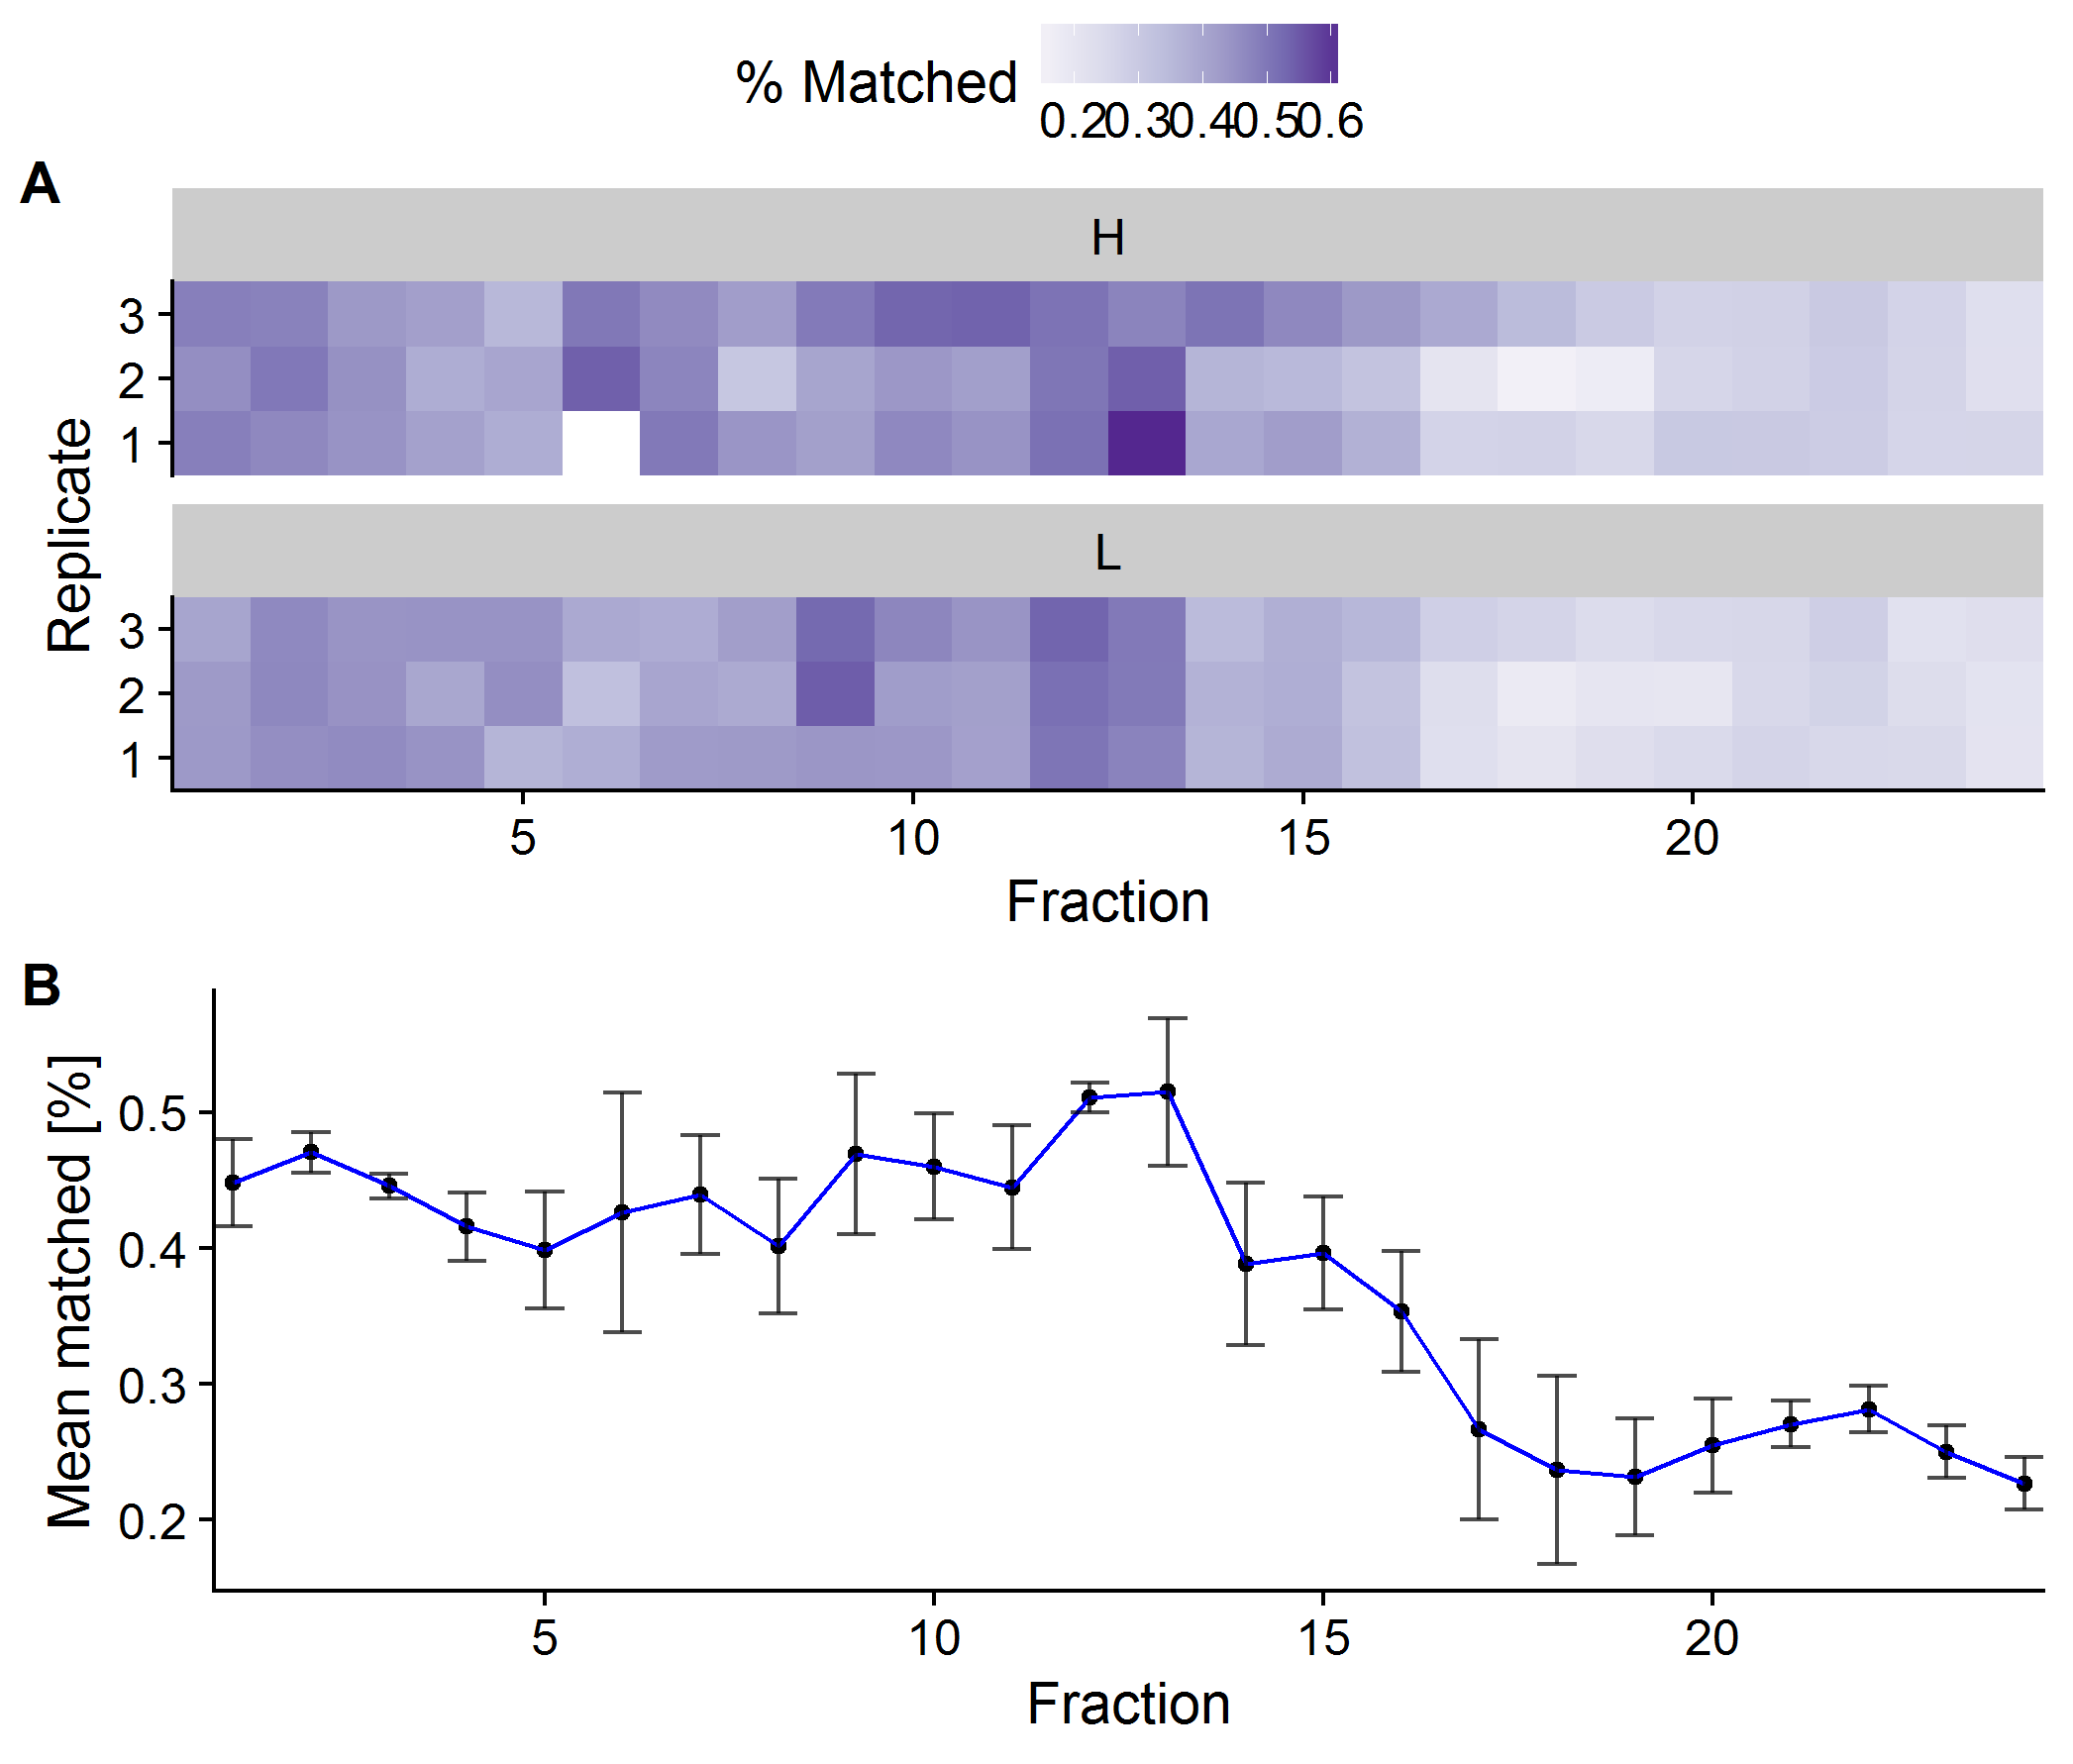
\includegraphics[width=0.8\textwidth]{match_percent}
\caption{Percentage of matched spectra in all samples. The total number of spectra per sample ranged between 5894 and 20249. \textbf{A} Percentages are encoded with a blue palette, the darker, the higher, and viceversa. \textbf{B} The mean for each analysed fraction across conditions and replicates is displayed together with error bars to represent the standard deviation. The sixth fraction of the first replicate in condition H was missing in the PRIDE data repository.}
\label{fig:match_percent}
\end{figure}

\subsection{Protein inference}

\begin{table}[H]
\begin{tabular}{ccccc}
  \toprule
 Total peptides & Unique peptides & Non-unique & Proteins & Protein groups \\ 
  \midrule
 46595 & 27384 & 19211 & 25056 & 10039 \\
 \bottomrule
\end{tabular}
\caption{\textbf{Protein inference results}. The counts of the different molecular entities detected by peptideShaker are displayed.}
\label{tab:quantification_table}
\end{table}

A total of 46595 peptides were inferred to be present in at least one of the fractions. Of them more than 27 thousand mapped to a unique protein. However, a significant amount mapped to more than one protein. Such peptides are called non-unique peptides. The 25056 detected proteins were grouped into 10039 protein groups. Protein groups are peptide generating entities for which enough data to confirm the presence of at least one of them is available, but not to exactly assess which of them. Thus, protein inferene algorithms create them when a does not uniquely map to a protein becuase it is not possible to distinguish which protein it truly comes from. Protein grouping decreased the amount of  considered protein entities to 10039.

Protein groups are very frequent due to several factors. For example, protein isoforms, consisting of protein sequences differing in potentially only one aminoacid, are very difficult to resolve. PeptideShaker executes a smart protein grouping by harnessing the annotation of proteins and classifying protein groups based on how well the annotation backs the protein group.

However, in the present analysis the quality of the protein group was not taken into account, as explained in the Materials and Methods.


\subsection{MBR and apex intensity extraction quantification}

The match between runs step allowed for increased identifications by transferring successful matches between replicate runs. The results of this process for the 13th fraction of the L condition is shown in figure \ref{fig:mbr}.

\begin{figure}[H]
\centering
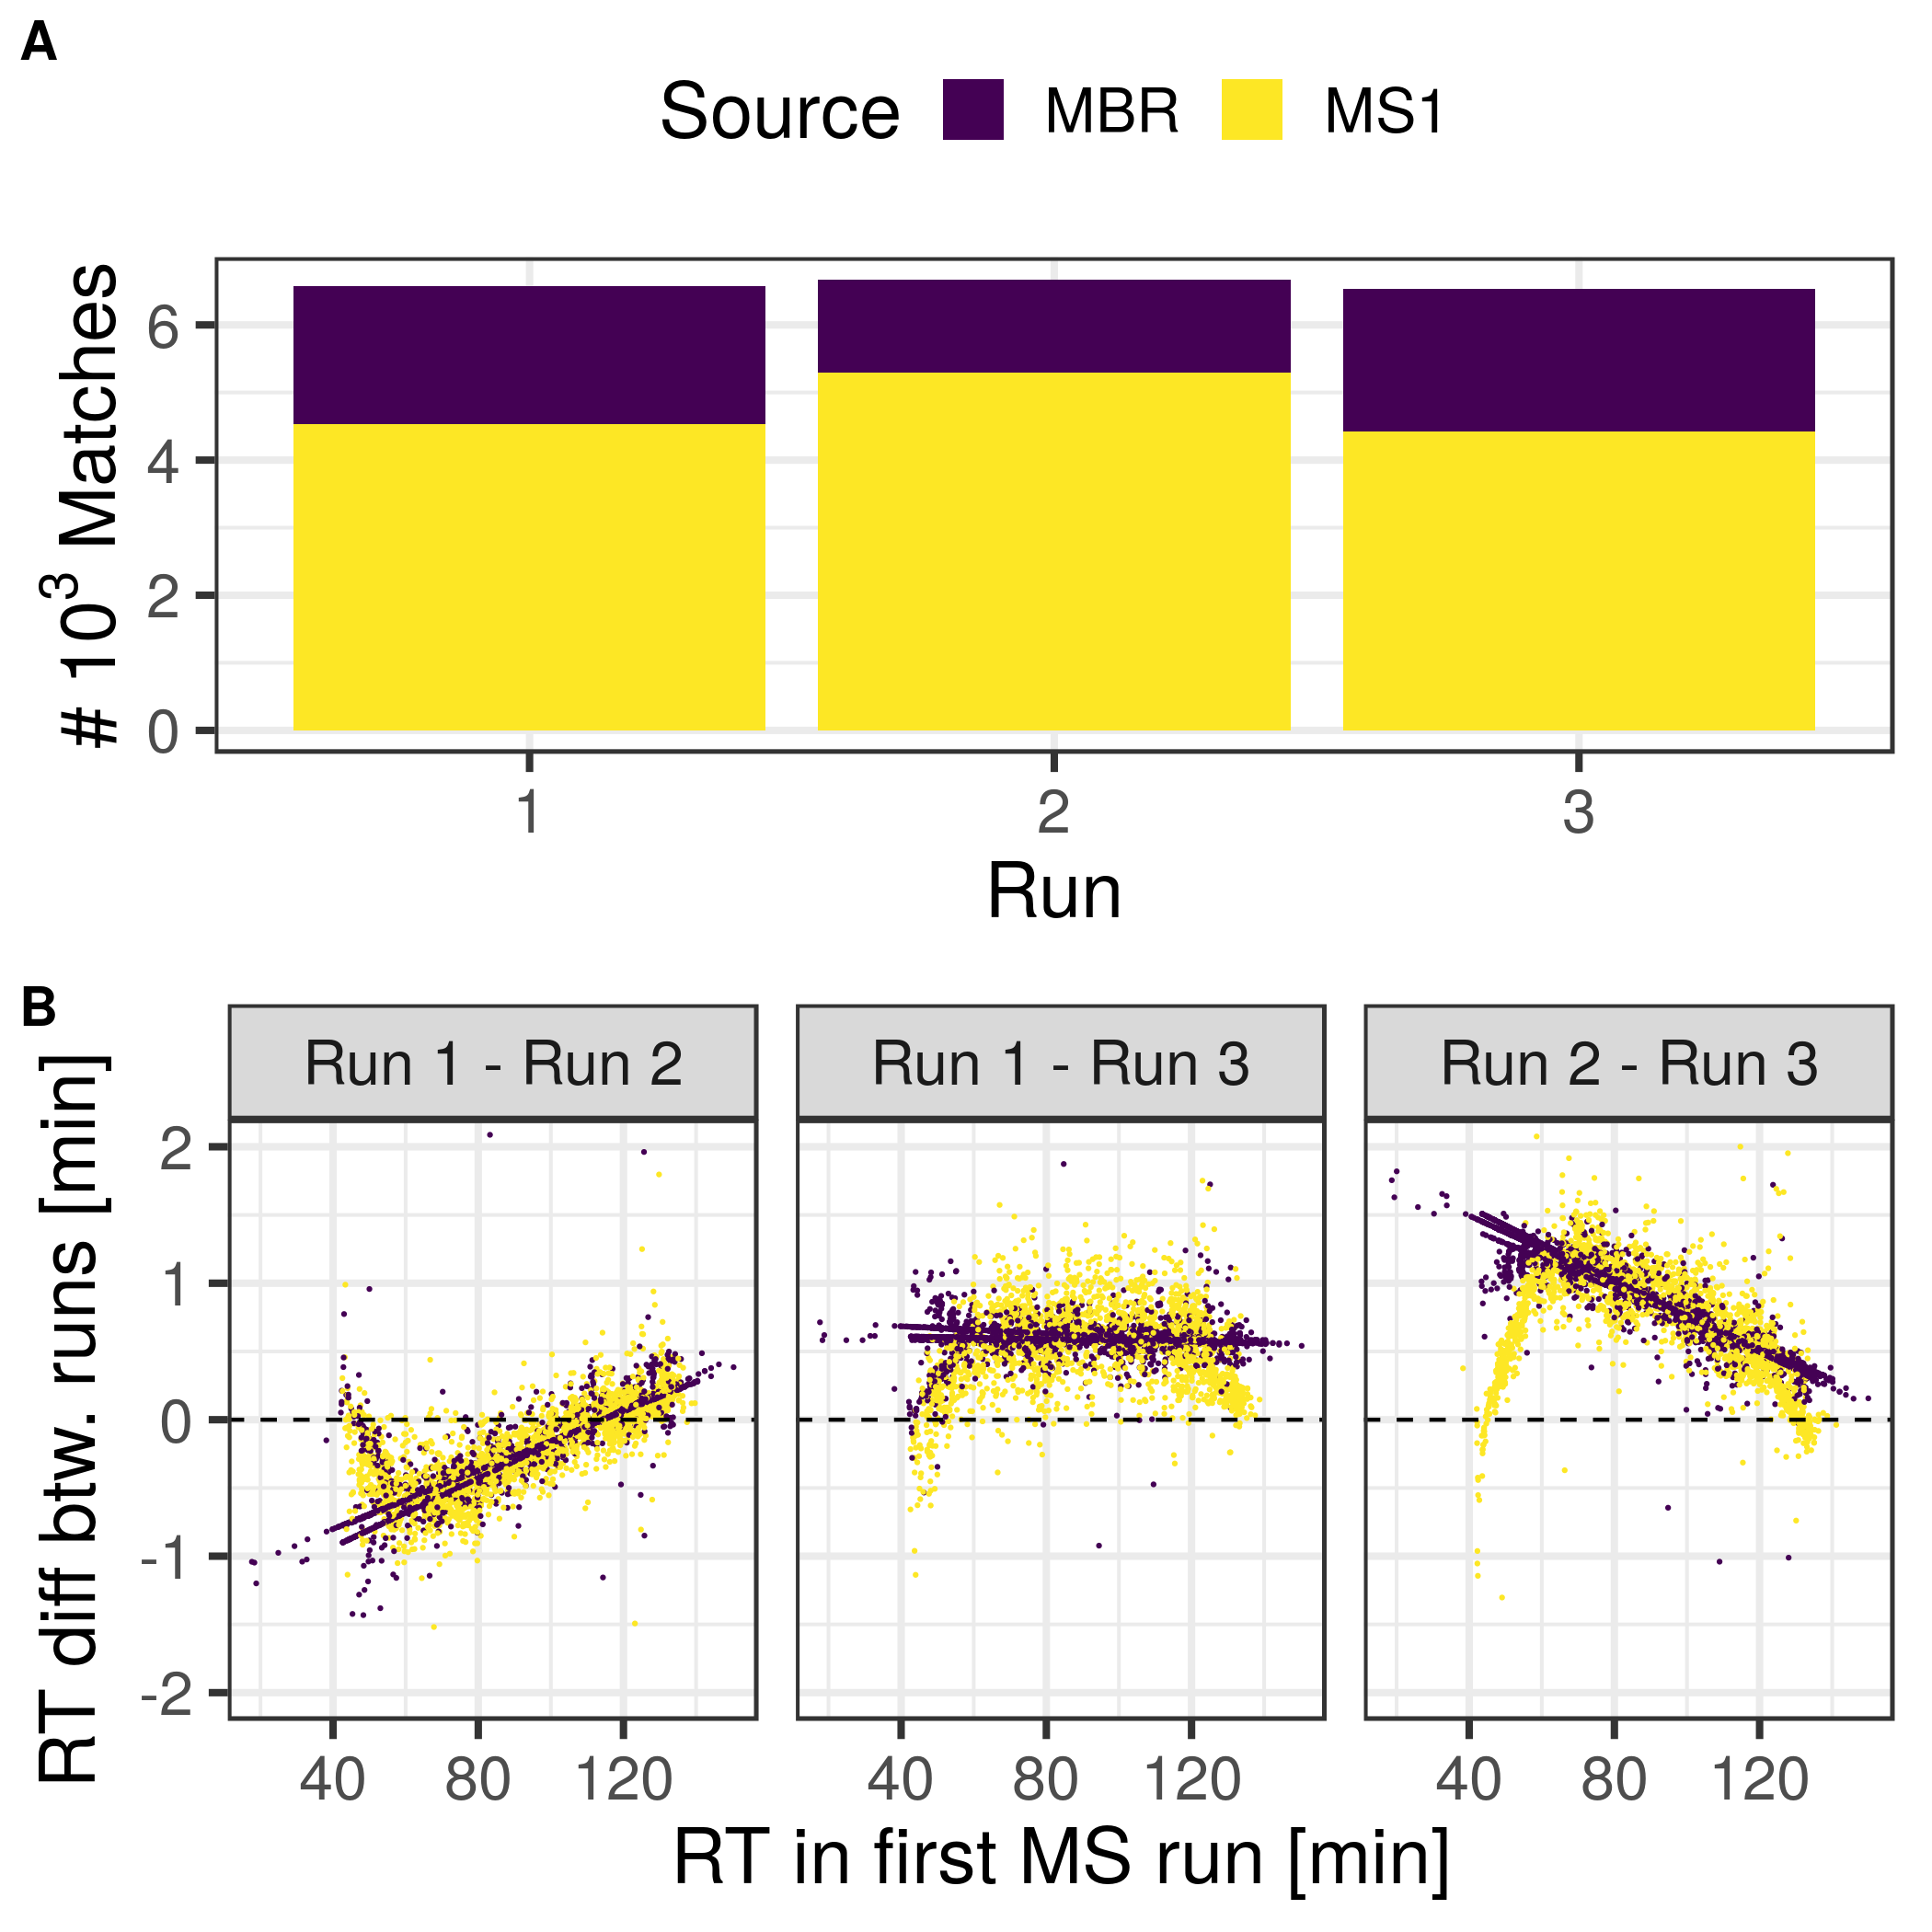
\includegraphics[width=\textwidth]{mbr_combined}
\caption{Match Between Runs with moFF. \textbf{A} Count of identifications on each run segreagated by source. More than 4k spectra were identified and validated by SearchGUI+peptideShaker. In this particular case, hundreds of new identifications were accomplished. \textbf{B} Match visualization. Every dot represents a peptide shared across 2 runs. The coordinate system illustrates its retention time on the first run on the x axis and the difference with the second run on the y axis. The color depicts whether the identification was carried out during the PSM process (MS1), or thanks to a cross-identification achieved by the MBR module (MBR).}
\label{fig:mbr}
\end{figure}

Once as many identifications as possible were gathered, a refinement of the measured MS1 intensity can be implemented to select the apex of every peak cluster, which yields robust intensity measurements for each sample (see figure \ref{fig:apex_intensity}). 

\begin{figure}[!h]
\begin{subfigure}{.9\textwidth}
  \centering
    \caption*{A}
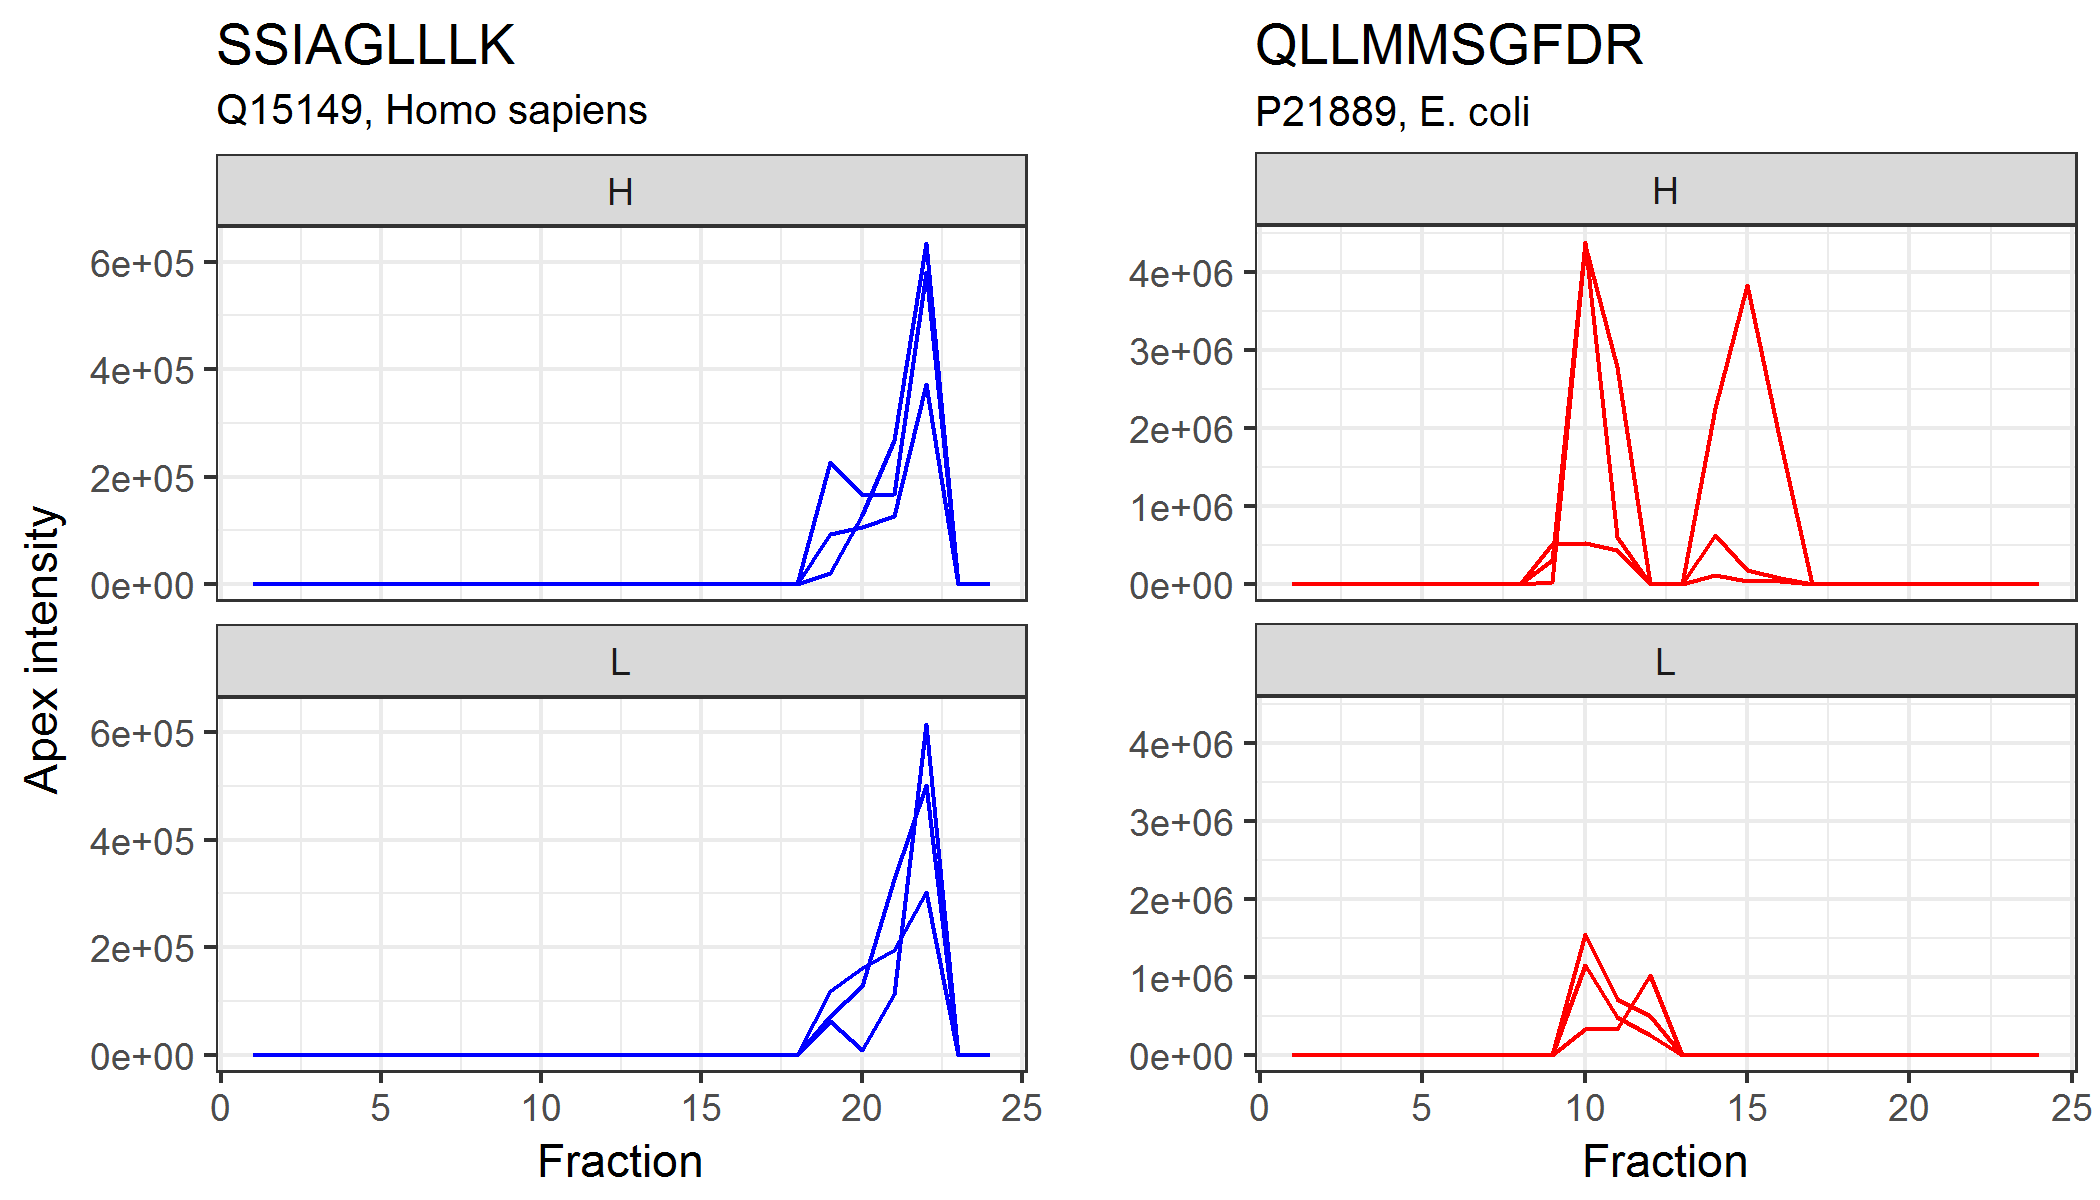
\includegraphics[width=.9\linewidth]{peptide_profile}
\end{subfigure}
\bigskip

\begin{subfigure}{.9\textwidth}
  \centering
    \caption*{B}
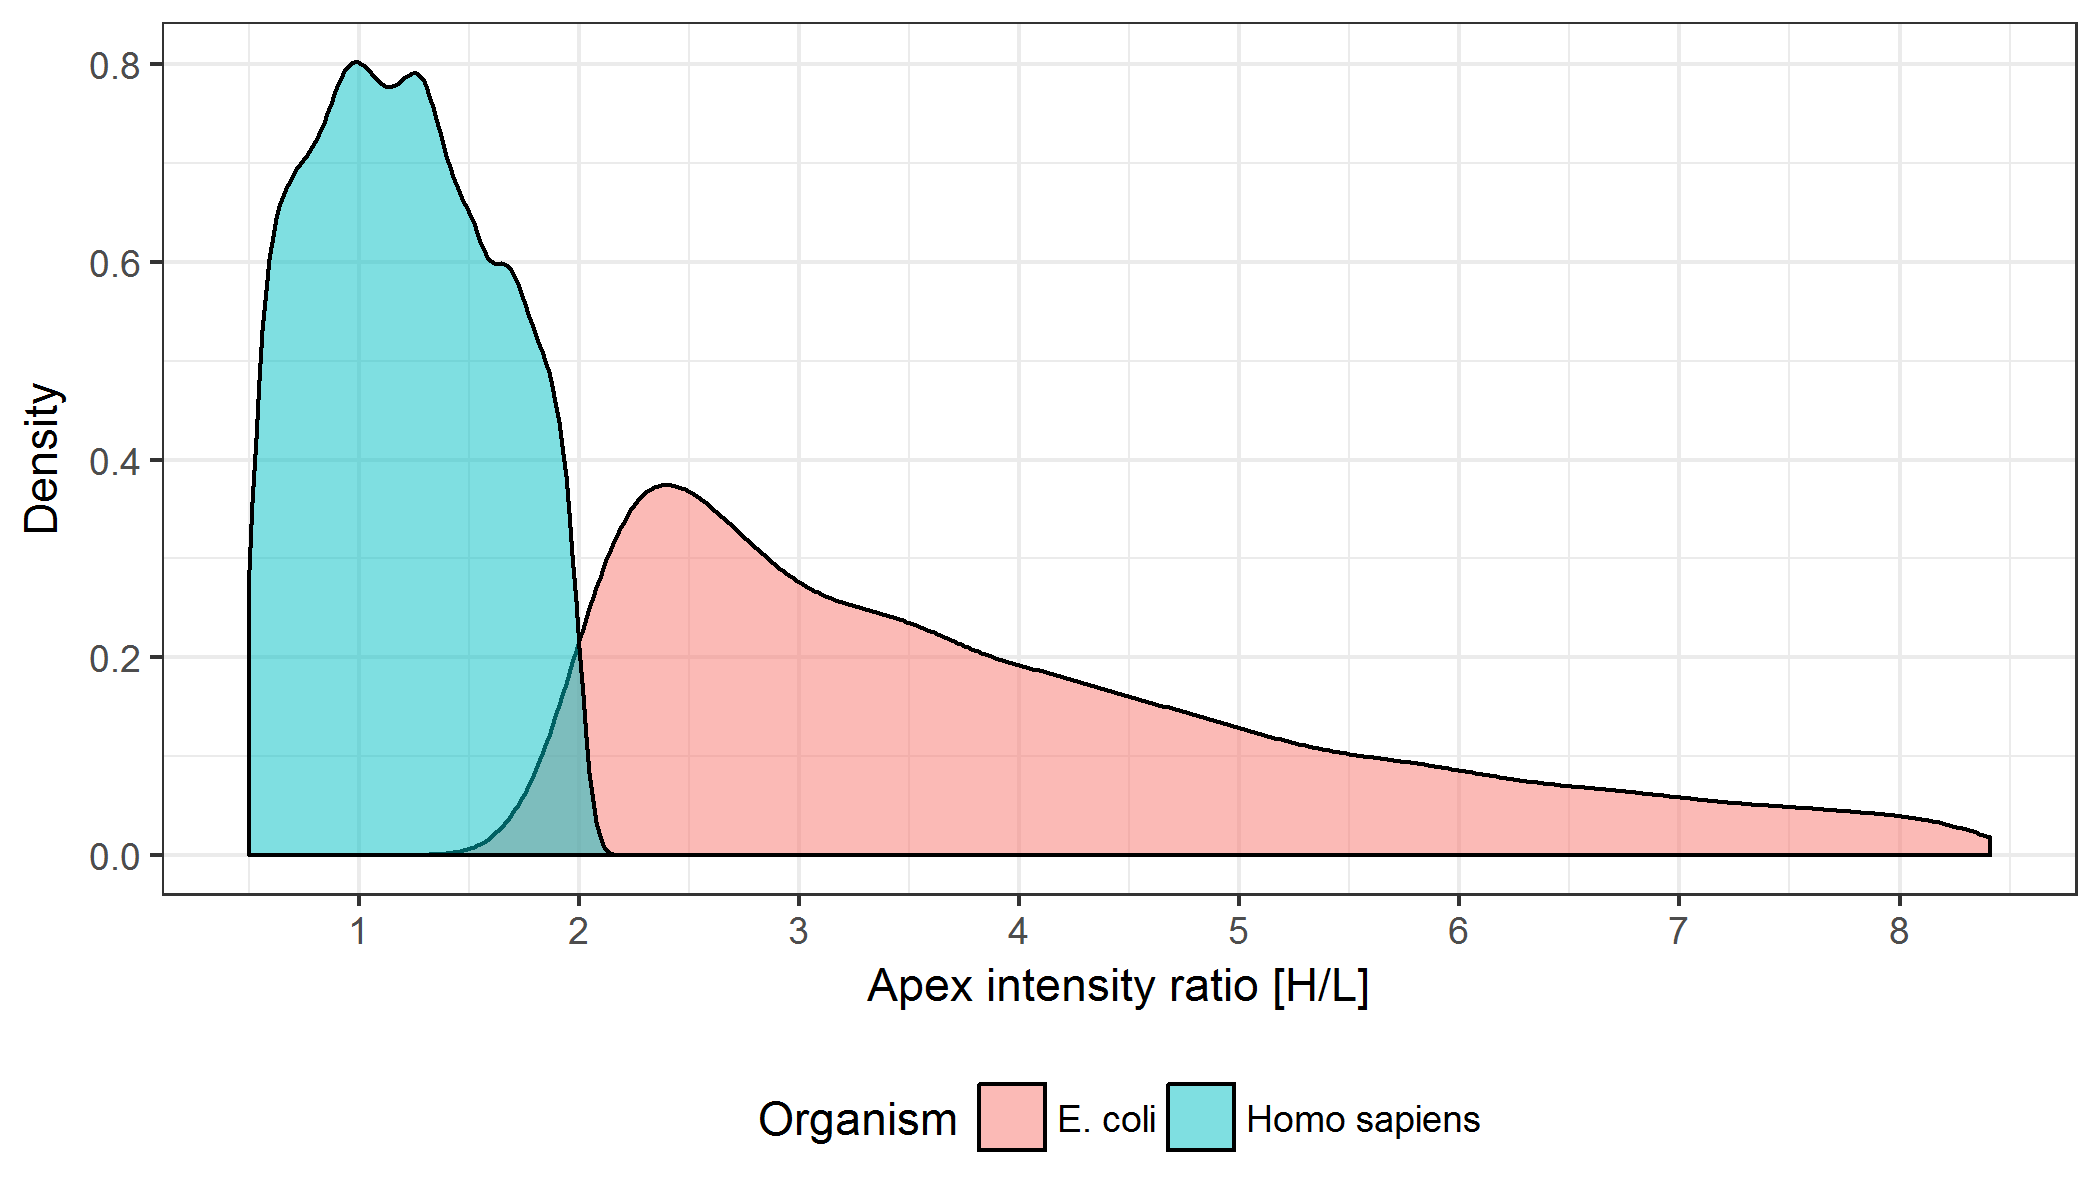
\includegraphics[width=.9\linewidth]{density_ratio}
\end{subfigure}
\caption{\textbf{A} The apex intensity profile across fractions for 2 different peptides, one from \textit{Homo sapiens}, and one from \textit{E. coli}. The figure illustrates the intrinsic intensity variability between technical replicates, particularly in the case of the \textit{E. coli} QLLMMSGFDR peptide, as it was almost non-existent in one of the runs. \textbf{B} The expected pattern of overall similar intensities for the \textit{Homo sapiens} data and 3-fold higher intensities for the \textit{E. coli} data in condition H was observed, confirming an acceptable performance of the protocol.}
\label{fig:apex_intensity}
\end{figure}


\subsection{Quantification}
\label{subsec:quantification}

The extracted apex MS1 intensities were used as proxy for peptide abundance to estimate protein $log_2$(ratios), or \textit{log2-fold-changes} across condition H and condition L. During quantification, it is important to take into account as many of the effects influencing protein quantification. In this case, besides the different H and L conditions, peptide, run and fraction effects could be distinguished. The MSqRob quantification engine treats effects differently depending on whether or not they are random, or fixed. Fixed effects should have a consistent impact in the ion currents measured in the spectrometer, whereas random effects are truly random and thus unpredictable.

The result of the process was the successful quantification of 5307 protein groups out of 10039 (see table \ref{tab:quantification_table}).

% latex table generated in R 3.4.4 by xtable 1.8-2 package
% Sun Jul 15 18:17:23 2018
\begin{table}[ht]
\centering
\begin{tabular}{llll>{\itshape}l}
  \toprule
 & log2FC & qval & Protein & Organism \\ 
  \midrule
1 & -4.76E-01 & 1.42E-24 & P78527 & Homo sapiens \\ 
   \rowcolor[gray]{0.95}2 & 6.80E-01 & 6.75E-24 & P0A8V2 & E. coli \\ 
  3 & 8.50E-01 & 4.39E-22 & P25516 & E. coli \\ 
   \rowcolor[gray]{0.95}4 & 7.07E-01 & 2.05E-18 & P63284 & E. coli \\ 
  5 & 1.04E+00 & 1.21E-17 & P37095 & E. coli \\ 
   \rowcolor[gray]{0.95}6 & 7.78E-01 & 1.51E-16 & P13029 & E. coli \\ 
  7 & 8.89E-01 & 5.62E-16 & P77804 & E. coli \\ 
   \rowcolor[gray]{0.95}8 & 8.53E-01 & 1.72E-15 & P23721 & E. coli \\ 
  9 & -6.97E-01 & 1.41E-14 & P09874 & Homo sapiens \\ 
   \rowcolor[gray]{0.95}10 & 1.37E+00 & 1.41E-14 & P37666 & E. coli \\ 
   \bottomrule
\end{tabular}
\caption{Results of the quantification pipeline. The 10 protein groups with the lowest \textit{q-val}  as estimated by MSqRob are shown. Notably, eight correspond to proteins belonging to \textit{E.coli}. The two human proteins exhibited in both cases an absolute value of the log2FC below 1.}
\label{tab:quantification_table}
\end{table}

The performance of the quantification can be evaluated thanks to the experimental design of the dataset. Since the \textit{E. coli} proteome was mixed on a 3:1 ratio in condition H, a log2FC of $log2(3)=1.58$ is expected for proteins coming from this organism. Likewise, human proteins should have a log2FC of 0. As such, the evaluation can be reformulated as a classification task were the quantification algorithm tries to distinguish between proteins coming from one or the other organism.

Some of the most frequent evaluations of the performance of a binary classiffier are Receiver Operating Characteristic (ROC) and Precision-Recall (PR) curves \cite{Bradley1997}, which demonstrate the performance of the algorithm at different cutoff values of a predictor variable. Together, they show the False Positive Rate (FPR), the True Positive Rate (TPR) or recall, and the precision exhibited by the algorithm.

\begin{figure}[!h]
\centering
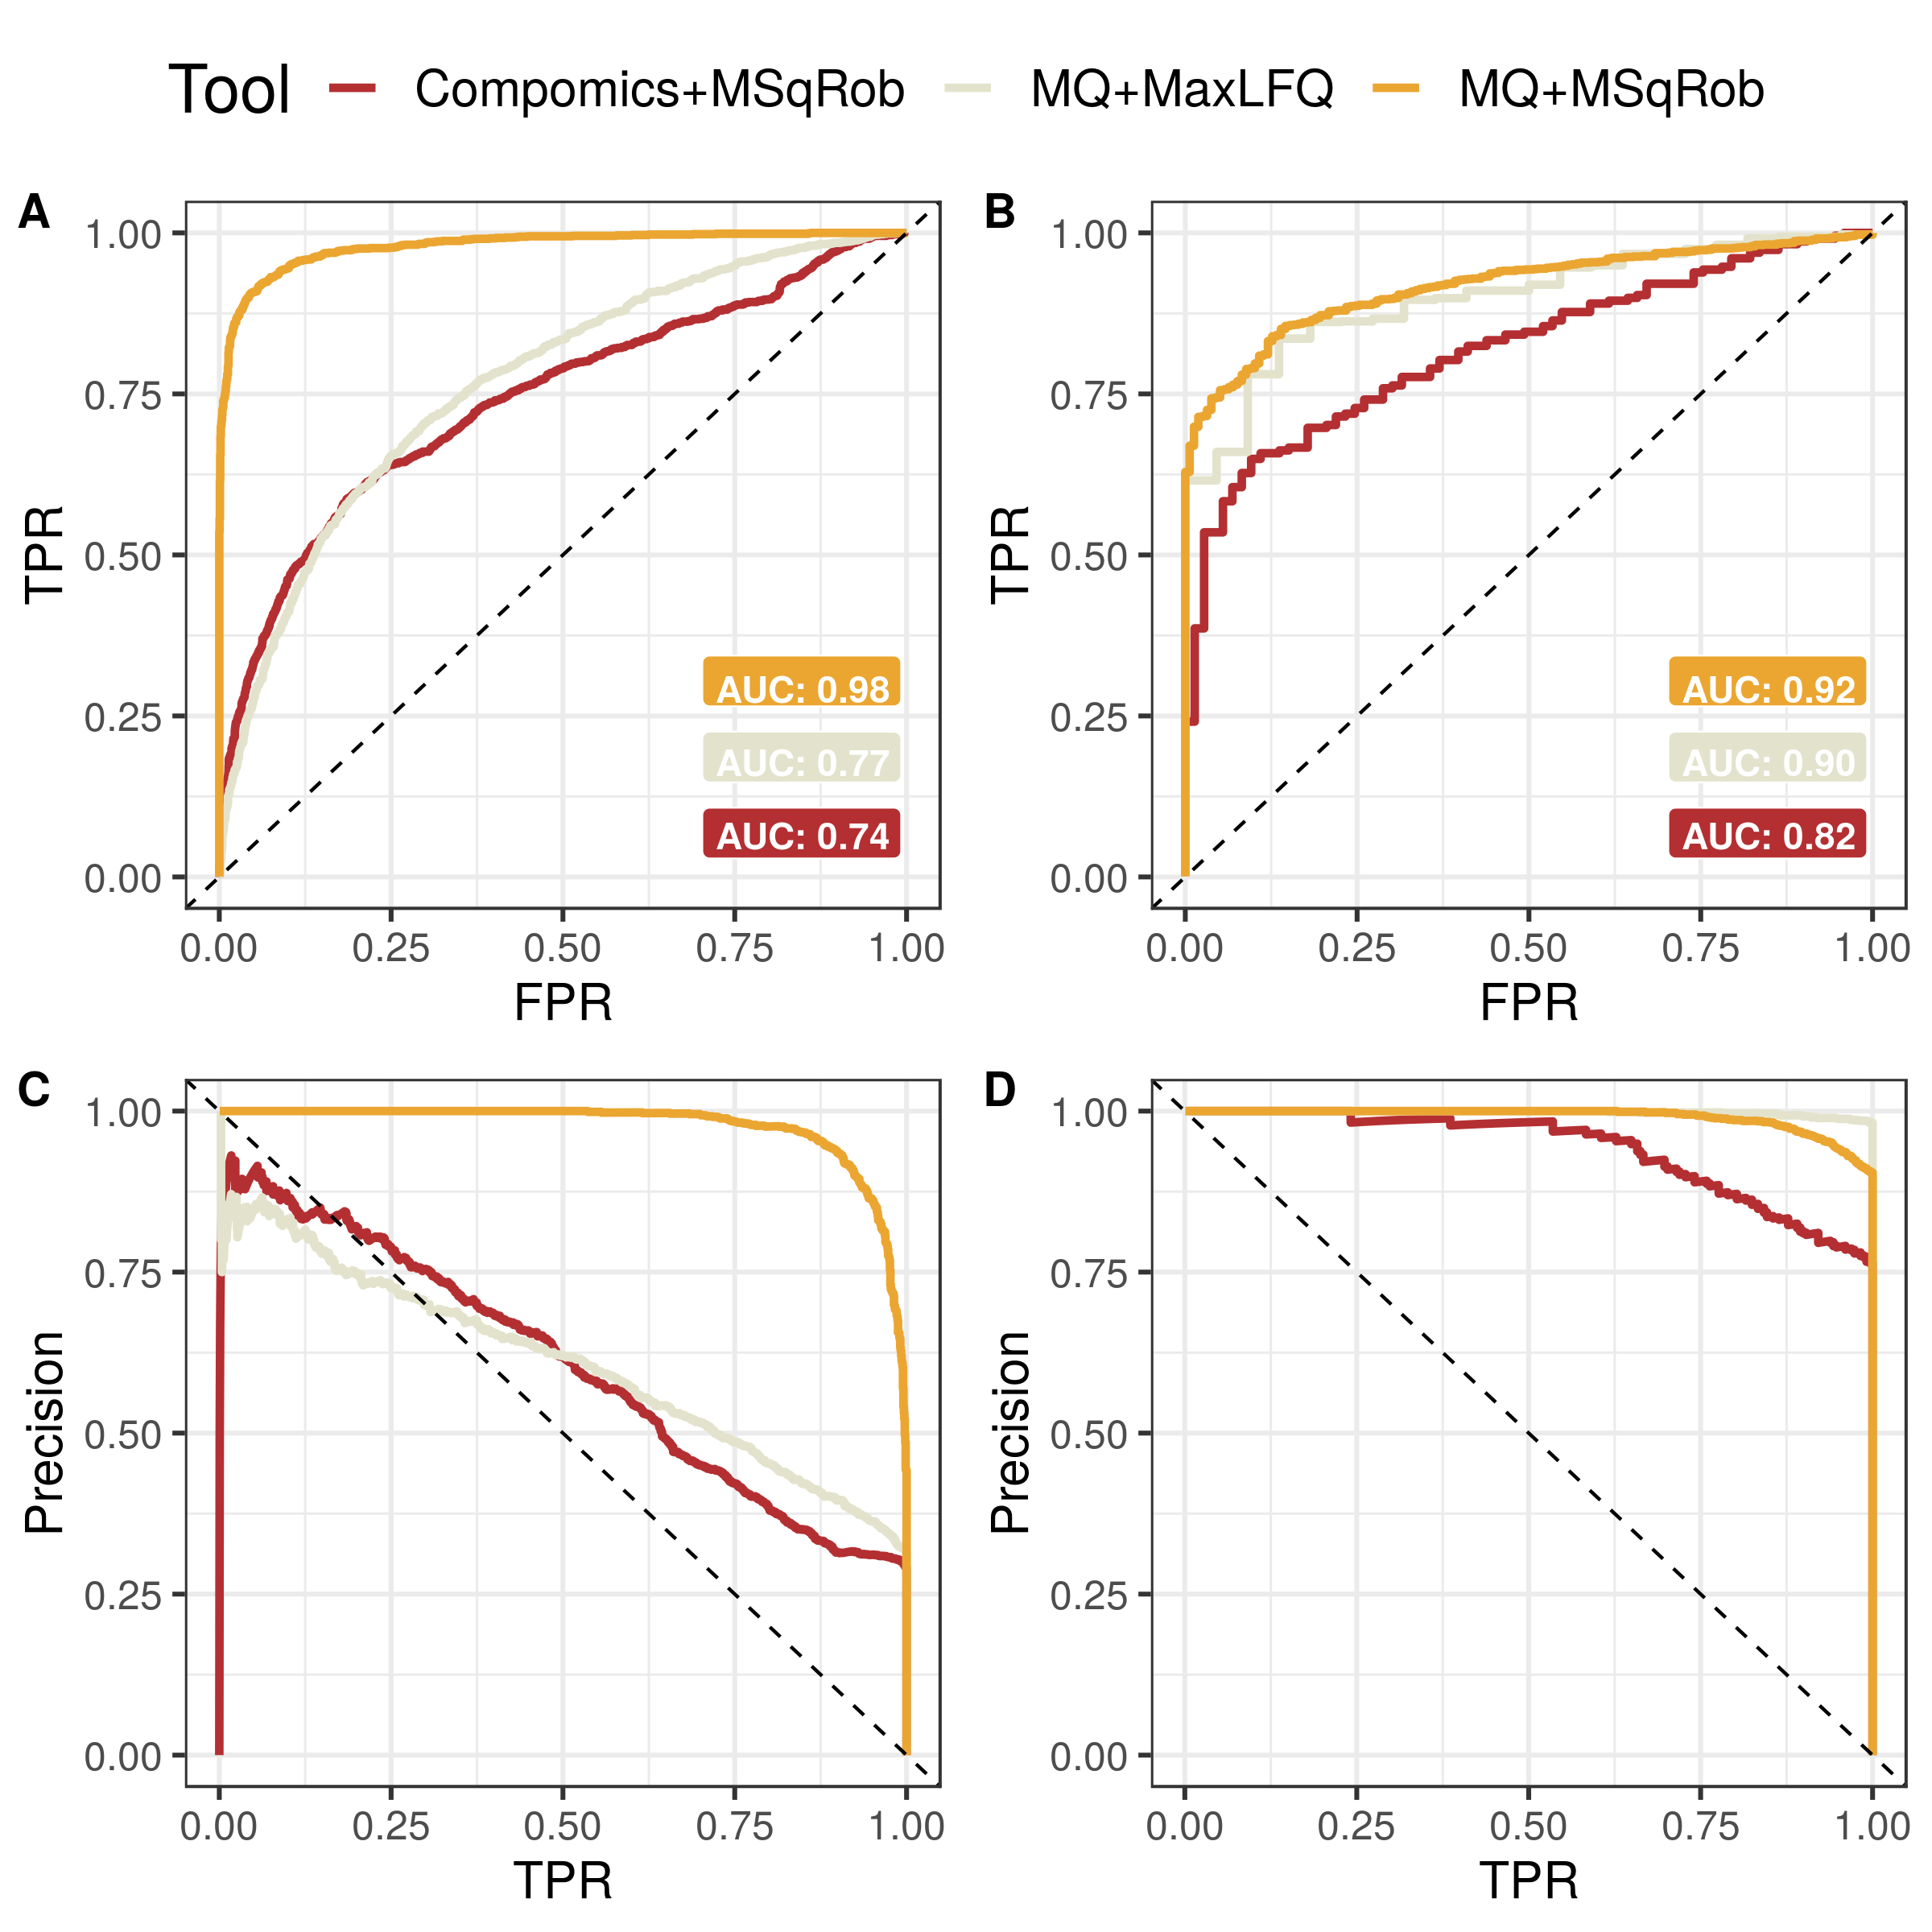
\includegraphics[width=\textwidth]{curves_plot}
\caption{ROC and PR curves displaying the behaviour of 3 different label-free quantification pipelines publicly available. \textbf{Compomics+MSqRob} is the pipeline presented in the previous sections. \textbf{MQ+MaxLFQ} consists a standard MaxQuant upstream analysis combined with its LFQ quantification engine. Finally, MQ+MSqRob blends MaxQuant upstream analysis with the MSqRob quantification engine. \textbf{A, B} ROC curve produced by the three algorithms with no log2FC filter, and keeping proteins with log2FC greater than 1, respectively. \textbf{C, D} PR curve produced by the three algorithms with no log2FC filter, and keeping proteins with log2FC greater than 1, respectively.}
\label{fig:roc_curves}
\end{figure}



In the present problem, they can be used to show how good the \textit{q-val} associated to a protein group is at separating the two proteomes. Thus, \textit{E. coli} proteins are treated as positives, and those from \textit{Homo sapiens} are treated as negatives. Moreover, a filter based on the log2FC can be applied to enrich the data in positives and facilitate the classification task.
In order to compare the results of the here presented pipeline (Compomics+MSqRob) with those achieved by other available tools, the analysis was repeated using the data processing implemented in MaxQuant \cite{Cox2008} at different steps. The pipeline combining MaxQuant and MaxLFQ (MQ+MaxLFQ) was fully carried out using the MaxQuant suite, whereas the combination of MaxQuant and MSqRob (MQ+MSqRob) used MaxQuant up to the fraction normalization step.

The result of this analysis is shown in figure \ref{fig:roc_curves}). Remarkably, Compomics+MSqRob achieved similar results to those resulting from MQ+MaxLFQ. Nonetheless, the latter performed clearly better when the log2FC filter was applied, indicating that a combined fold change and q-value criteria is best for declaring proteins as differentially abundant. In all cases MQ+MSqRob was as good as MQ+MaxLFQ, if not much better.

\begin{figure}[!h]
\centering
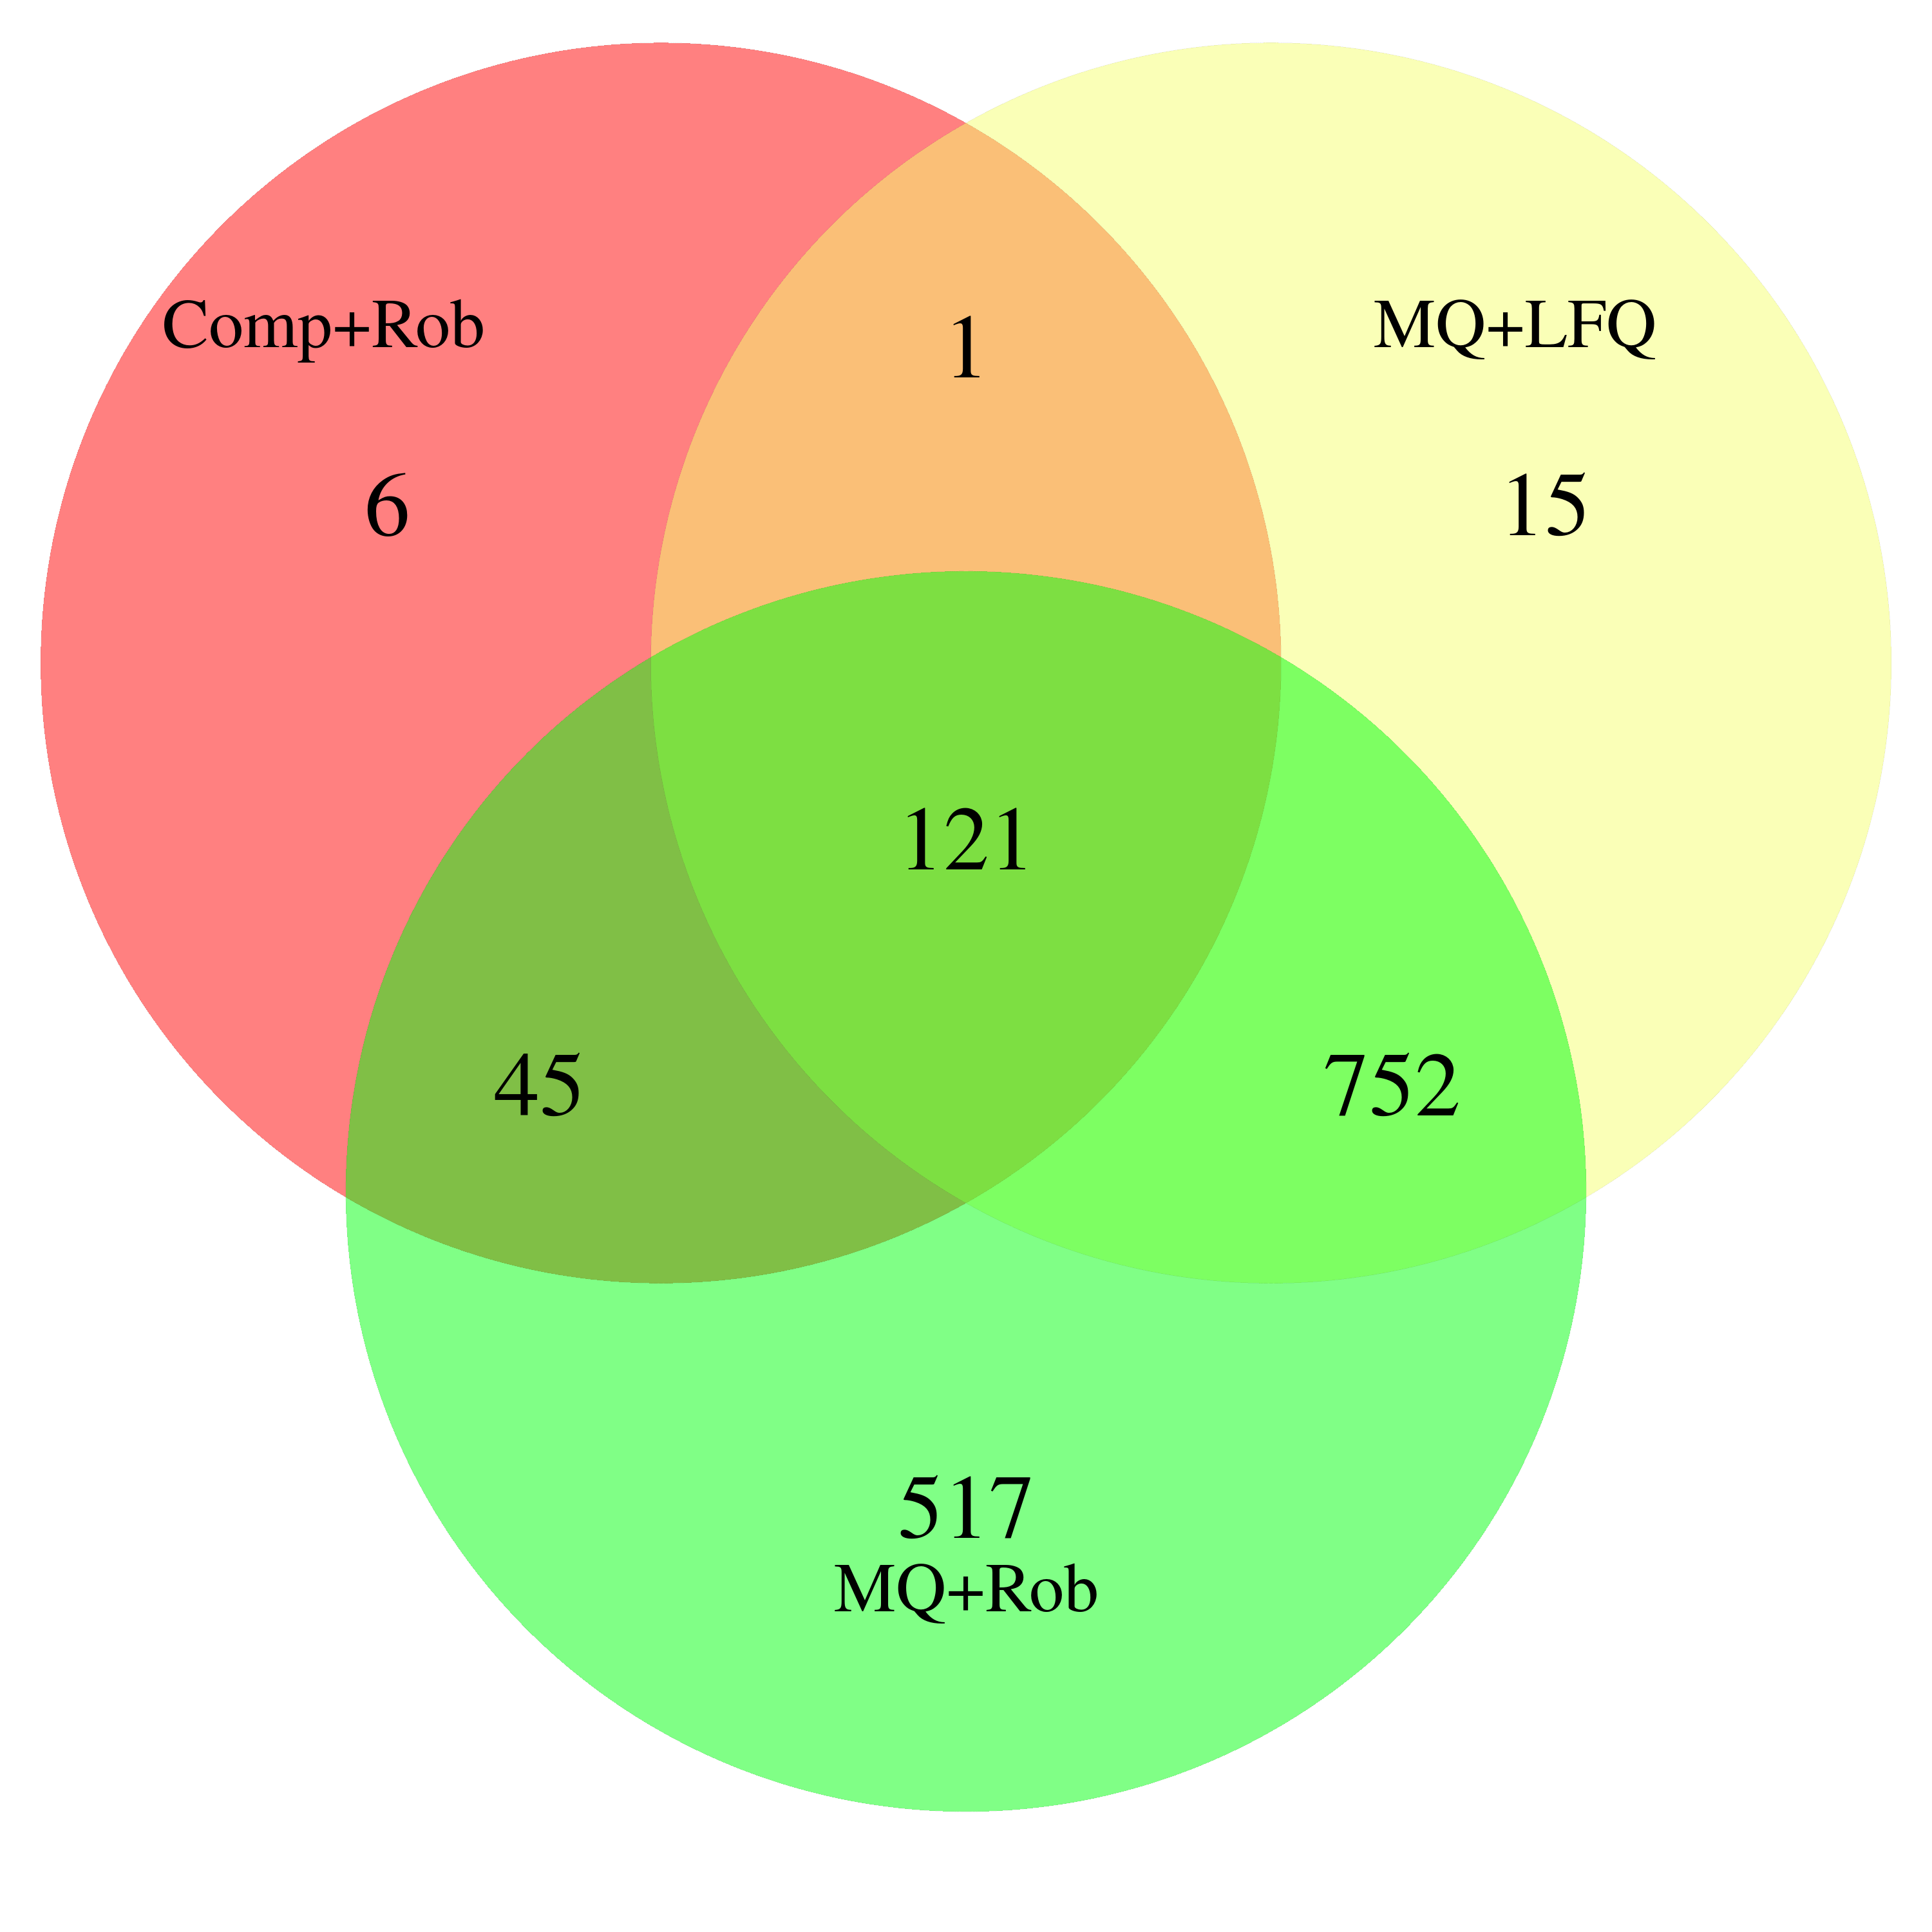
\includegraphics[width=0.8\textwidth]{vennDiagram}
\caption{Agreement between the different pipelines. The Venn diagram displays the number of \textit{E. coli} proteins found to be differentially abundant by each pipeline.}
\label{fig:venn}
\end{figure}


In order to visualize the level of agreement of the pipelines for the assignment of differentially abundant proteins, a Venn diagram was constructed (see figure \ref{fig:venn}). Venn diagrams provide a straightforward visualization of the overlap of several ensembles of proteins. The scrutiny of the counts reveals a high degree of agreement, with most proteins detected by Compomics+MSqRob or MQ+MaxLFQ being detectd by MQ+MSqRob too. Remarkably, 517 proteins were detected by MQ+MSqRob alone, which further confirmed its resolving power.


Additionally, the accuracy with which each program assigns a log2FC estimate to each protein group, and how significantly different from the null value of 0 it was found to be, provides further insights on the pros and cons of each pipeline, as shown in figure \ref{fig:combined_plot}. This analysis confirmed that the pipeline providing the best separation between organisms was MQ+MSqRob.




\begin{figure}[!h]
\centering
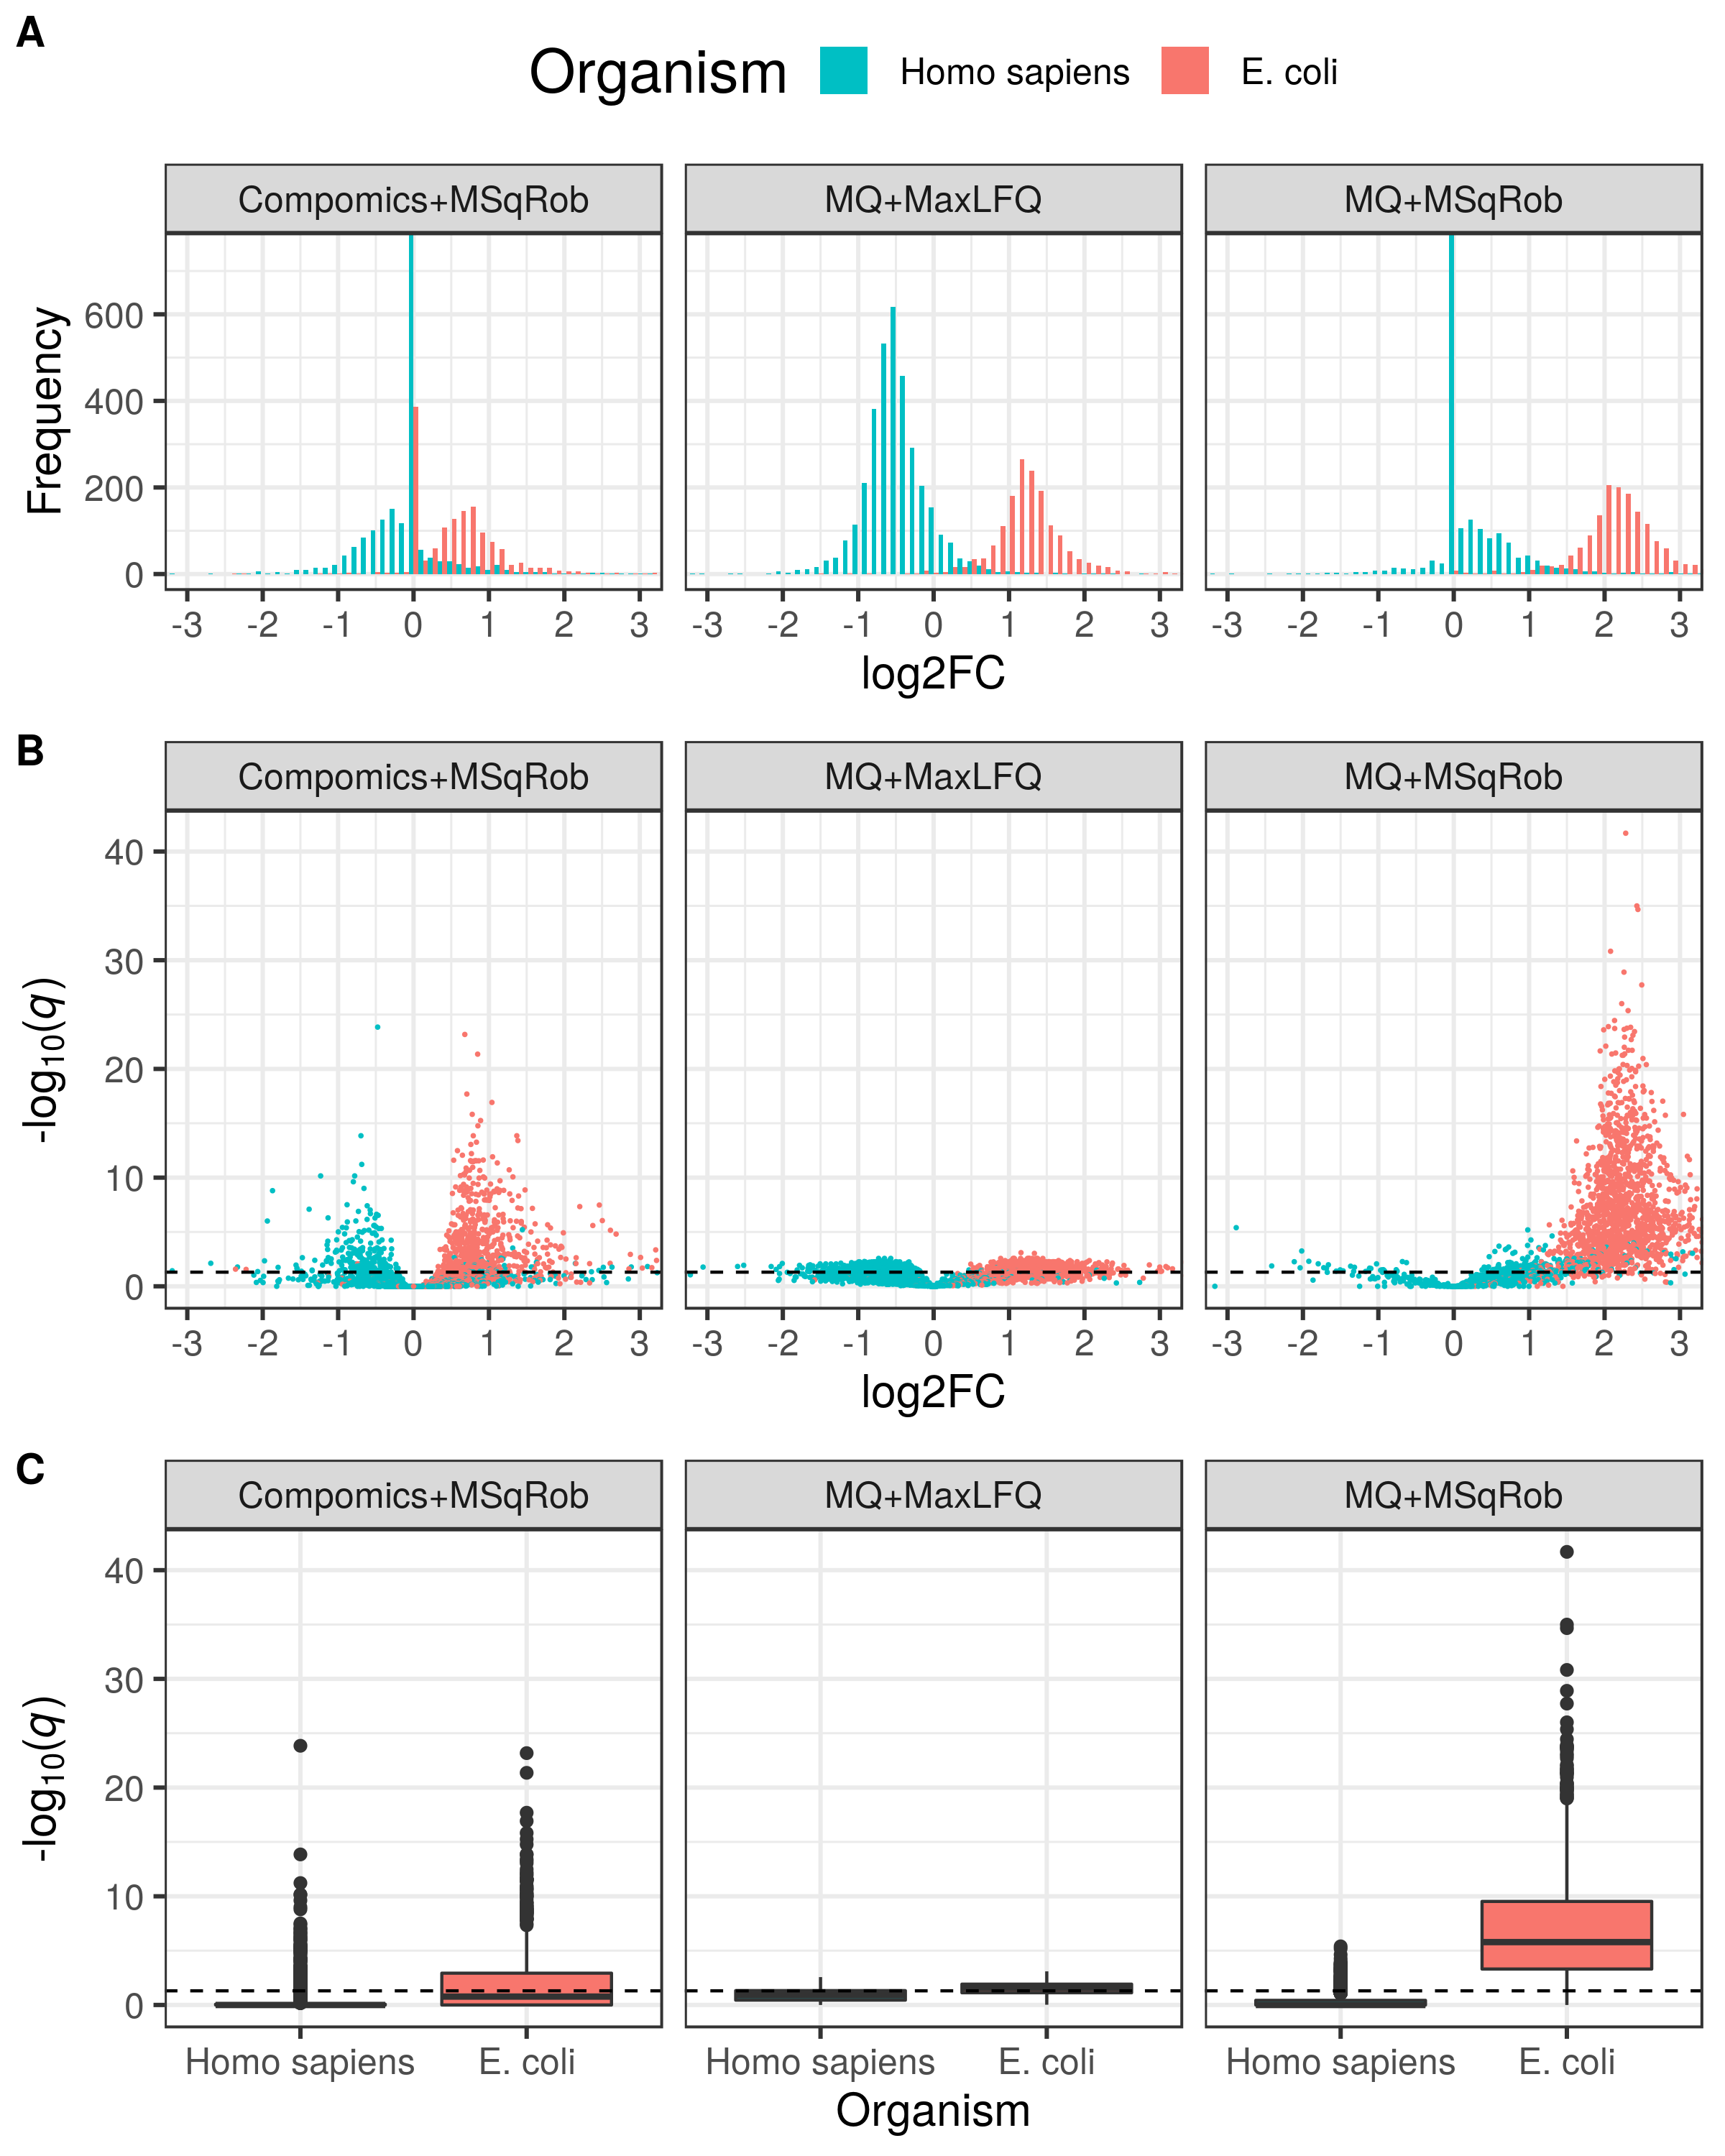
\includegraphics[width=\textwidth]{combined_plot}
\caption{Overview over the different pipelines performance. Quantification results are segregated by the source organism. \textbf{A} Histogram of the log2FC estimates. \textbf{B} Volcano plot, where every protein group is represented by a dot and the coordinates map to its log2FC on x and the minus logarithm of the q-value on y. \textbf{C} Boxplots of the minus logarithm of the q-value distribution.}
\label{fig:combined_plot}
\end{figure}



\section{Discussion}

\subsection{Improvement of the PSM step}

The low attained matching rate manifests existing room for improvement in the currently available tools. Remarkably, it has been shown that the combined usage of multiple search engines can increase identifications, since the different statistical frameworks implemented in each of them compensate each other\textquotesingle s caveats. Furthermore, \textit{de novo} search engines are available and supported by SearchGUI, and the latest developments in the field, like the IdentiPy engine \cite{Levitsky2018} are progressively incorporated to the framework \footnote{\href{https://github.com/compomics/peptide-shaker/issues/309}{https://github.com/compomics/peptide-shaker/issues/309}}. Their usage is predicted tor improve identification rates and quality of the matches.

The most important reason why many spectra remain unidentified is the presence of post-translational modifications (\ac{PTM}s), which exponentially increase the search space, forcing most workflows to discard many of the peptides featuring a PTM. New approaches to the problem are emerging, mainly machine learning methods for the handling of unexpected modifications \cite{Gabriels}. Moreover, the prediction of \ac{MS2} peak intensities patterns from peptide sequences promises to increase the amount of evidence available during the PSM process, thus boosting correct identifications \cite{Kirik2018} \cite{Degroeve2013}.

Finally, the extremely low matching rates in the latter fractions translated to decreased contributions to the number of identifications. This indicated that decreasing the number of fractions would not have had a major impact in the experiment\textquotesingle s depth.



\subsection{Improvement of the feature extraction step}

While the apex intensity is a good estimate of the peptide abundance, other methods are available that could potentially provide more robust data, such as the area of the peak. This is the approach taken by the recently published tool RawQuant \cite{Kovalchik2018}, or the feature detection tool in the OpenMS pipeline \cite{Sturm2008}. 

\subsection{Improvement of the quantification step}

The deployed relative quantification approach successfully manages to estimate the log2FC of several of proteins in the dataset with high confidence. However, it was not found to be the best performing of the assayed pipelines in the benchmark dataset. Several axes of improvement are clear from the results.

\subsubsection{Management of sample fractionation}

Sample fractionation allows for a deeper analysis of the peptide mix, which in turn leads to increased identifications and an increased amount of data to be analyzed. However, it psimultaneously provides an extra random effect that difficults quantification if not handled properly.

The way the MaxLFQ engine solves the problem is by aggregating the data from the same sample across fractions using a ponderated average. One normalizing weight is determined for every sample via the \textit{Levenberg-Marquant minimisation of the overall proteome variation} $H(N)$ as defined in \cite{Cox2014}. A custom implementation was written in Python using the scipy module, but the results were not satisfactory.

MSqRob treats the fractions as a random effect, as explained in section \ref{subsec:quantification}. As a consequence, the statistical model in MSqRob can be overwhelmed by the resulting inconsistency, and eventually provide null estimates of the ratio. This is clearly manifested in figure \ref{fig:combined_plot} as the bins at log2FC of 0, which represent protein groups for which MSqRob did not find enough evidence to discard the null hypothesis. While no \textit{E. coli} proteins fell in this category in the MQ-MSqRob pipeline, many did in the Compomics+MSqRob, proving room for improvement in this aspect.

In any case, the way sample fractionation is handled should depend upon the fractionation method. For example, membrane fractionation can be exploited when working with membrane proteins \cite{Marmagne2006}.

To sum up, the presently implemented fraction handling is correct and provides good results, but fine-tuning of the pipeline at this step is expected to improve the results of the quantification. Thanks to the open-source nature of the software, this is indeed possible.


%which is defined according to the following expressions:
%
%\begin{equation}
%I_{P,A}(\text{N}) = \sum\limits_{j=1}^{k}{\text{N}_{A,j} \times \text{XIC}_{P,A,j}}
%\end{equation}
%
%where $\text{N}_{A,j}$ stands for the normalization coefficient for sample $A$ and fraction $j$, and $\text{XIC}_{P,A,j}$ stands for the extracted ion current in the same sample and fraction for peptide P. The sum runs over all k fractions.
%
%\begin{equation}
%H_P(N) = \sum\limits_{A,B} \abs{\log(\frac{I_{P,A}(N)}{I_{P,B}(N)})}^2
%\end{equation}
%
%\begin{equation}
%H(N) = \sum\limits_{p} H_p(N) 
%\end{equation}
%
%where the pair $A$ and $B$ is any of the sample pairs where peptide $P$ is detected. The overall proteome variation is 


\subsubsection{The pitfalls of mass spectrometry}

The application of mass spectrometry to proteomics is a very hot topic in research, driving innovations in the way the different components of the spectrometer work. One recent example is the development of the timsTOF\texttrademark\xspace Pro (Trapped Ion Mobility Spectrometry-Time Of Flight) system by Bruker, which supports PASEF (Parallel Accumulation and SErial Fragmentation) spectrometry \footnote{\href{https://www.prnewswire.com/news-releases/bruker-launches-the-timstof-pro-mass-spectrometer-to-enable-the-revolutionary-pasef-method-for-next-generation-proteomics-300520791.html}{https://www.prnewswire.com/news-releases/bruker-launches-the-timstof-pro-mass-spectrometer-to-enable-the-revolutionary-pasef-method-for-next-generation-proteomics-300520791.html}}. Notwithstanding, it reveals the immature state of the technology. Slight inconsistencies in the protein extraction and digestion, bias in the peptide ionization, presence of unexpected PTMs, and detector saturation and insensitivity, remain as problems contributing to the eventual measurement variability characteristic of mass spectrometry \cite{Piehowski2013}. Thus, adequate cleaning of the peptide dataset, and care to ignore outliers is preeminent. Indeed, the input file for the MQ+MaxLFQ consisted of a preprocessed file which removed the most problematic proteins \cite{Cox2014}, which explains why more than 500 extra proteins could be quantified when using MSqRob (see figure \ref{fig:venn}).

\subsubsection{Support for absolute quantification}

While relative quantification like that performed by MSqRob is enough to infer differential abundance of proteins across conditions, absolute quantification would provide an estimate of protein quantities that would support many other analyses, and facilitate comparison between datasets, in a way similar to what the normalised read counts in FPKM (Fragments Per Kilobase per Million Reads) does in transcriptomics. On the other hand, MaxLFQ provides absolute estimates, albeit less robust.

\subsubsection{Quantification of uncertainty}

All the quantification approaches enunciated until now make use of different frequentist approaches to the problem, that evaluate how significantly different the data are from what would be expected under a null hypothesis of a null ratio across the pair of conditions. Yet, it does not provide probabilistic interpretations of the uncertainty behind the estimate. The development of a Bayesian framework which endeavors at solving this issue is presented in chapter \ref{chap:model}.


\section{Conclusion}

An open-source, free, platform-agnostic and customisable label-free relative quantification pipeline assembling publicly available tools was presented in this work. The pipeline is capable of providing qualitative information on the protein composition of a sample using the latest proteomics search engines and validation software. Moreover, it can be extended to support more complex tasks, like \textit{De novo} search, or the study of \ac{PTM}s, thanks to its non-monolithic nature and usage of open-formats. Likewise, the openness of the data in all steps allows for quality control checks along the way. However, the comparison against other workflows shows the room for improvement in the quantification step when dealing with fractionated data, albeit deficiencies in this aspect should have no impact in non-fractionated datasets.



\chapter{BayesQuant: Probabilistic estimation of protein ratios}
\label{chap:model}

\section*{Summary}

The current label-free quantification methods, reviewed in section \ref{sec:quantification} all rely on frequentist statistics, which return point estimates of model parameters such as the estimate of the abundance ratio (fold change) across conditions. However, a Bayesian based approach to this problem, that we know of, is lacking in the literature. As a response to this shortcoming, a statistical model implemented in the probabilistic programming framework Pymc3 was developed and tested on the same benchmark dataset from chapter \ref{chap:pipeline}). The execution of the three steps required when doing Bayesian modelling, mainly (I) model implementation, (II) computation of posterior probabilities and (III) model checking, will be described for this particular problem in the present chapter, together with a discussion on its usability and its strengths.

\section{Introduction}

Both the LFQ and MSqRob quantitication engines presented in chapter \ref{chap:pipeline} took a frequentist approach to the problem of protein quantification. Such approaches, establish a null hypothesis, complementary to the actual hypothesis being tested (alternative hypothesis). The information about the phenomena being modelled is put to use to measure how likely this null hypothesis is via Null-Hypothesis Significance Testing (NHST).


\begin{align}
H_0: & \log_2(FC) = 0 \nonumber \\
H_1: & \log_2(FC) \neq 0 \nonumber
\end{align}

The results of this analysis will depend not only of the observed data, but also the data generation process \cite{Kruschke}. This way, both tools returned point estimates of the $\log_2$(FC) between a pair of conditions and a p-value, which provides a measurement of the probability of the null hypothesis. The null hypothesis usually states that the true value of the parameter is 0. Thus, p-values do not say anything about probability of the alternative (our) hypothesis.

The Bayesian statistical framework provides an alternative point of view by revolving the role played by the model parameters and the observed data. While frequentist statistics treats the data as random and the parameters as fixed, a Bayesian framework swaps their roles and yields a probability distribution for any model parameter given the provided data. Bayesian analyses rely on the observed data and prior knowledge about the phenomenon only, and comes equipped with an equation that mathematically formalizes how to introduce these two dependencies in a valid way. This is the so called Bayes-theorem.
 


\begin{figure}[!h]
\centering
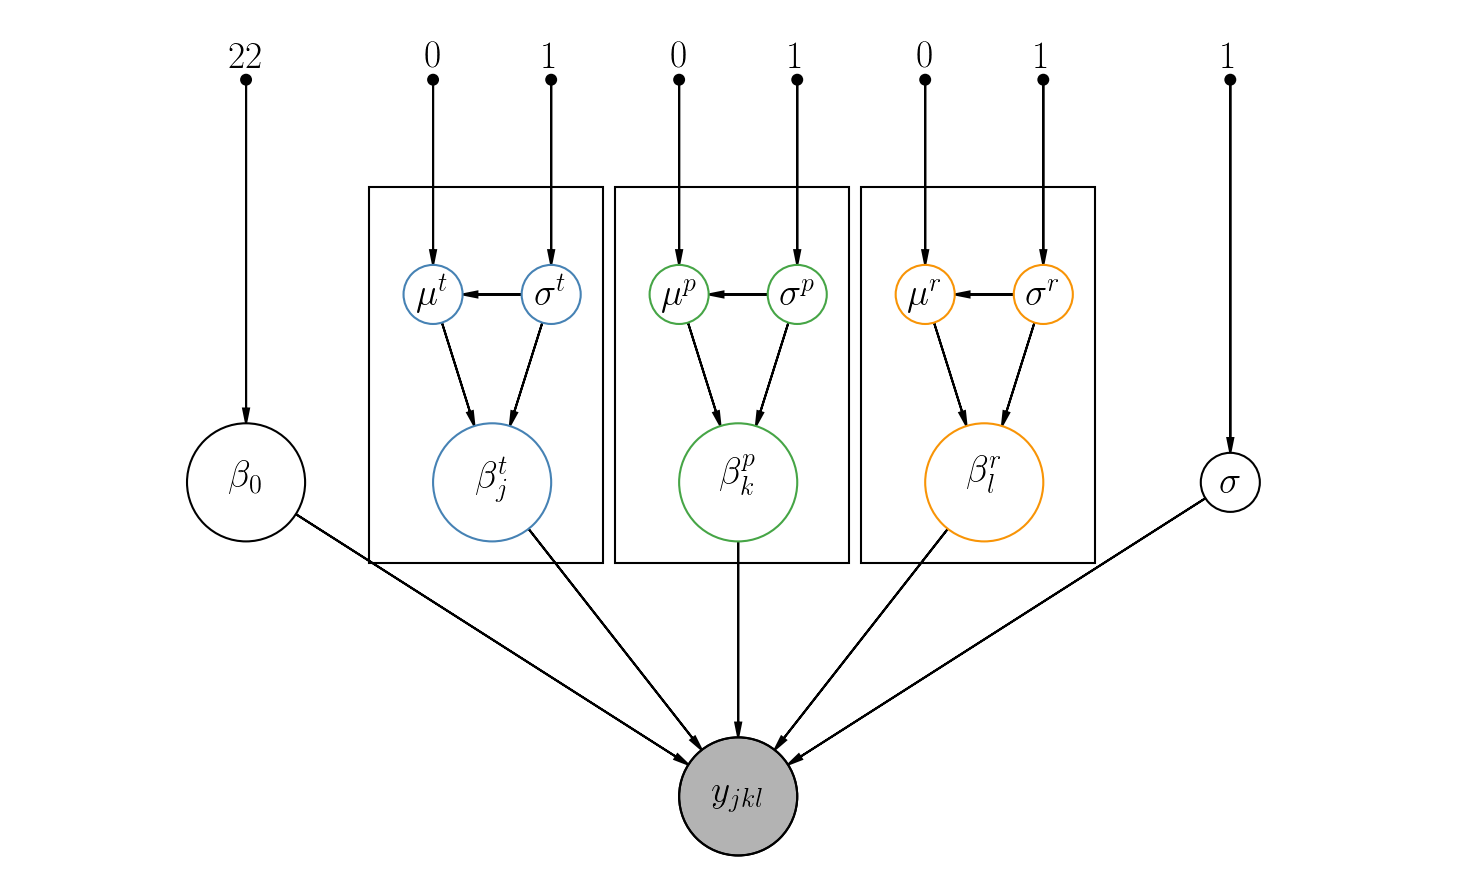
\includegraphics[width=\textwidth]{graph}
\end{figure}

%As such, they are the target of multiple regulatory pathways ensuring their quantities are kept within homeostatic ranges.



\chapter{Pipeline benchmarking on \ac{NZ} data}
\label{chap:benchmark}

\section*{Summary}

A benchmark dataset generated by \ac{NZ} technicians was run through the pipeline presented in chapter \ref{chap:pipeline} to showcase its performance. The experiment consisted of the application of two different treatments to THP-1 cell cultures. One group was subjected to an experimental procedure triggering the immunological response, while the other group was subjected to a negative control. The analysis of the resulting dataset through the aforementioned pipeline should thus reflect a change in the protein profile corresponding to an activation of the immune system in the first group when compared to the second. The results confirmed that the computational analysis successfully captured this response. It was concluded that the software can be used in future experiments where the expected biological phenomena is not known.



\chapter*{Conclusion}
\label{chap:conclusion}

\chapter*{Appendix}
\label{chap:appendix}

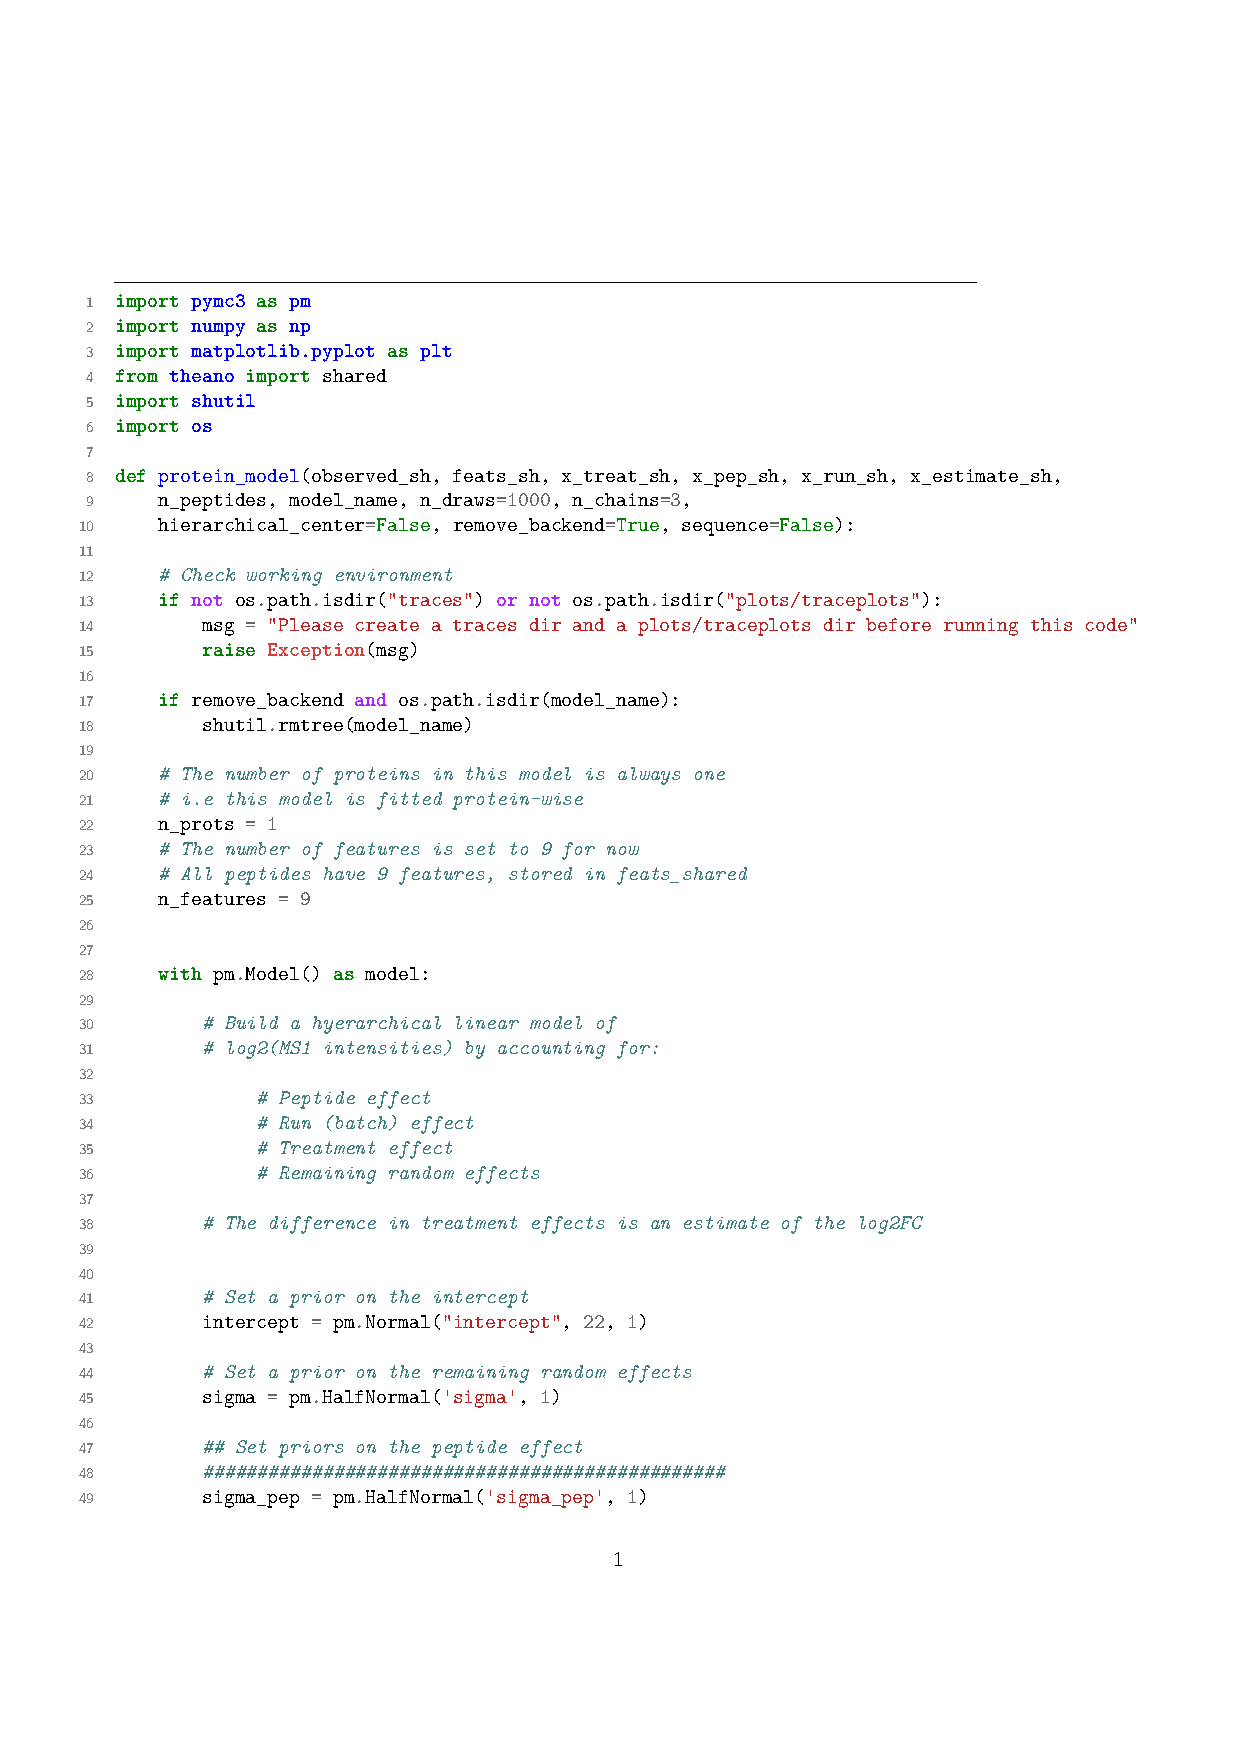
\includepdf[pages=-]{appendix.pdf}


\bibliographystyle{unsrt_etal}
\footnotesize{\bibliography{bibliography}}

\end{document}
%%  ==================================================================
%%  End document

